% Sidst opdateret: 14/1 1994
\chapter{Analyse af tidsr{\ae}kker}
Analyser af tidsr{\ae}kker kan give mange interessante
oplysninger om et ikke-line{\ae}rt dynamisk system. I dette
kapitel vil vi give et overblik over de forskellige
metoder, som er i brug.

\vspace{4.0mm}
Tidsr{\ae}kkeanalyse er ikke kun anvendelig i studiet af
oscillerende kemiske reaktioner, men kan bruges inden for
alle de omr{\aa}der, som besk{\ae}ftiger sig med
ikke-line{\ae}re dynamiske systemer.

\vspace{4.0mm}
En tidsr{\ae}kke kan kort defineres som en f{\o}lge af tal
(eller vektorer). Man vil ofte forestille sig en
tidsr{\ae}kke som f{\o}lgen $\vec{x}_1, \ldots, \vec{x}_N$,
hvor indekset hentyder til en disketisering af tiden.
P{\aa} den m{\aa}de kan tidsr{\ae}kken ogs{\aa} skrives som
$\vec{f}(t_1), \ldots, \vec{f}(t_N)$.

\vspace{4.0mm}
Tidsr{\ae}kker fremkommer derfor naturligt ved et
eksperiment. Man m{\aa}ler med passende mellemrum
forskellige st{\o}rrelser; i kemien kunne det v{\ae}re
koncentrationen af et bestemt stof. Man ser ogs{\aa} ofte,
at diskretiseringen af tiden er foretaget s{\aa}ledes, at
m{\aa}lingerne foretages med lige store mellemrum, hvilket
vi i dette kapitel har antaget.

\vspace{4.0mm}
Andre grene af naturvidenskaberne og de teknologiske
videnskaber anvender ogs{\aa} forskellige teknikker til
analyse af tidsr{\ae}kker. F.eks.\ er det en generel (og
velkendt) metode i statistik, men ofte arbejder
statistikere ikke med systemer, som kan udvise en kaotisk
opf{\o}rsel [\citen{chatfield}]. Inden for
signalbehandling findes der ogs{\aa} en del forskellige
teknikker, som kan bruges eller bliver brugt
[\citen{NumRec,Bendat71,Gold69,Lawes84}].

\newpage
\section{Fourier-metoder}
Som n{\ae}vnt i indledningen, findes der indenfor
signalbehandling forskellige metoder. En af de vigtigste er
klassen af Fouriermetoder (ogs{\aa} kaldet
spektralmetoder). Selv om disse metoder ogs{\aa} anvendes i
andre sammenh{\ae}nge end denne afhandlings emne, vil vi
dog komme med et par eksempler p{\aa} deres styrke.

\vspace{4.0mm}
Grundideen i Fouriermetoderne er at skrive tidsr{\ae}kken
$\{x_j\}_{j=0}^{n-1}$ som en Fourierr{\ae}kke
[\citen{Prag:Arno}]. Med andre ord, {\o}nsker vi at finde
koefficienter $\{d_j\}_{j=0}^{n-1}$ s{\aa}

\begin{equation}
  \label{tid:FFT}
  x_k = \sum_{j=0}^{n-1} d_j e^{2\pi i j/n}.
\end{equation}

Ovenst{\aa}ende er ikke en Fourierr{\ae}kken, men derimod
en endelig r{\ae}kke. En egentligt Fourierr{\ae}kke er
givet ved [\citen{MatF}]

\[
  \sum_{n \in \Z} c_n e^{inx},
\]

hvor koefficienterne $c_n$ er givet ved

\[
c_n = \frac{1}{2\pi}\int_{-\pi}^{\pi} f(x)e^{-inx} dx.
\]

Ovenst{\aa}ende r{\ae}kke er defineret for periodiske
funktioner, dvs.\ funktioner som opfylder $f(x+2\pi) =
f(x)$.

\vspace{4.0mm}
{\em Fast Fourier Transform} algoritmen er en meget
effektiv metode til at finde koefficienterne i ligning
\ref{tid:FFT}. I [\citen{NumRec}] beskrives en
implementation af denne metode. Som det kan ses af ligning
\ref{tid:FFT}, er tidsr{\ae}kken blevet transformeret fra
tidsdom{\ae}net til frekvensdom{\ae}net. Det
Fouriertransformerede signal kaldes ofte for et spektrum.

\vspace{4.0mm}
Tidsr{\ae}kken kan have forskellige opf{\o}rsler, og ud fra
det Fouriertransformerede signal er det muligt at finde ud
af r{\ae}kkens opf{\o}rsel. Nedenfor har vi opremset de
forskellige opf{\o}rsler og deres spektra [\citen{Prag:Arno}]

\begin{description}
  \item[Periodisk] En periodisk tidsr{\ae}kke vil have en
  hovedfrekvens samt alle dens overtoner, dvs.\ spektraet
  vil have en st{\ae}rk linie ved $f$ og svage linier ved
  $n\cdot f$. For en uendelig lang tidsr{\ae}kke vil
  linierne v{\ae}re Diracs deltafunktion, men for en
  endelig r{\ae}kke vil linierne have en endelig bredde.
  Bredden $h$ er givet ved $h\ge \frac{2\pi}{n\Delta t}$,
  hvor $n$ er antallet af datapunkter og $\Delta t$ er
  tiden mellem to m{\aa}linger. Figur \ref{tid:SinPer}
  viser grafen for $\sin \frac{j\pi}{50}$ for $j =
  1,\ldots, 1000$ og dens spektrum.


    \boxfigure{t}{\textwidth}{
      \begin{center}
        \begin{pspicture}(0,-0.6)(14,5)
          %  \psgrid[](0,0)(0,0)(14,10)
          \rput[tl]{*0}( 1.0,4.3){% GNUPLOT: LaTeX using TEXDRAW macros
\begin{texdraw}
\normalsize
\ifx\pathDEFINED\relax\else\let\pathDEFINED\relax
 \def\QtGfr{\ifx (\TGre \let\YhetT\cpath\else\let\YhetT\relax\fi\YhetT}
 \def\path (#1 #2){\move (#1 #2)\futurelet\TGre\QtGfr}
 \def\cpath (#1 #2){\lvec (#1 #2)\futurelet\TGre\QtGfr}
\fi
\drawdim pt
\setunitscale 0.24
\linewd 3
\textref h:L v:C
\path (132 270)(795 270)
\path (132 51)(132 489)
\linewd 4
\path (132 94)(147 94)
\path (795 94)(780 94)
\move (115 94)\textref h:R v:C \htext{{\footnotesize$-0.8$}}
\path (132 138)(147 138)
\path (795 138)(780 138)
\move (115 138)\htext{{\footnotesize$-0.6$}}
\path (132 182)(147 182)
\path (795 182)(780 182)
\move (115 182)\htext{{\footnotesize$-0.4$}}
\path (132 226)(147 226)
\path (795 226)(780 226)
\move (115 226)\htext{{\footnotesize$-0.2$}}
\path (132 270)(147 270)
\path (795 270)(780 270)
\move (115 270)\htext{{\footnotesize$0.0$}}
\path (132 313)(147 313)
\path (795 313)(780 313)
\move (115 313)\htext{{\footnotesize$0.2$}}
\path (132 357)(147 357)
\path (795 357)(780 357)
\move (115 357)\htext{{\footnotesize$0.4$}}
\path (132 401)(147 401)
\path (795 401)(780 401)
\move (115 401)\htext{{\footnotesize$0.6$}}
\path (132 445)(147 445)
\path (795 445)(780 445)
\move (115 445)\htext{{\footnotesize$0.8$}}
\path (198 51)(198 66)
\path (198 489)(198 474)
\move (198 17)\textref h:C v:C \htext{{\footnotesize$100$}}
\path (331 51)(331 66)
\path (331 489)(331 474)
\move (331 17)\htext{{\footnotesize$300$}}
\path (464 51)(464 66)
\path (464 489)(464 474)
\move (464 17)\htext{{\footnotesize$500$}}
\path (597 51)(597 66)
\path (597 489)(597 474)
\move (597 17)\htext{{\footnotesize$700$}}
\path (729 51)(729 66)
\path (729 489)(729 474)
\move (729 17)\htext{{\footnotesize$900$}}
\path (132 51)(795 51)(795 489)(132 489)(132 51)
\linewd 3
\path (132 270)(132 270)(132 276)(133 283)(134 290)(135 297)
\cpath (135 304)(135 311)(136 318)(137 324)(138 330)
\cpath (138 337)(139 344)(140 350)(141 357)(141 363)
\cpath (141 369)(142 375)(143 381)(144 387)(144 393)
\cpath (145 399)(146 404)(146 409)(147 414)(147 420)
\cpath (148 424)(149 429)(150 434)(150 438)(151 443)
\cpath (152 447)(152 451)(153 455)(153 458)(154 462)
\cpath (155 465)(156 468)(156 471)(157 473)(158 476)
\cpath (158 478)(159 480)(159 482)(160 483)(161 485)
\cpath (162 486)(162 487)(163 488)(163 488)(164 489)
\cpath (165 489)(165 489)(166 488)(167 488)(168 487)
\cpath (168 486)(169 485)(169 483)(170 482)(171 480)
\cpath (171 478)(172 476)(173 473)(174 471)(174 468)
\cpath (175 465)(175 462)(176 458)(177 455)(177 451)
\cpath (178 447)(179 443)(180 438)(180 434)(180 429)
\cpath (181 424)(182 420)(183 414)(183 409)(184 404)
\cpath (185 399)(186 393)(186 387)(186 381)(187 375)
\cpath (188 369)(189 363)(189 357)(190 350)(191 344)
\cpath (192 337)(192 330)(192 324)(193 318)(194 311)
\cpath (195 304)(195 297)(196 290)(197 283)(198 276)
\cpath (198 270)(198 263)(199 256)(200 249)(201 242)
\cpath (201 235)(202 228)(203 222)(204 215)(204 209)
\cpath (204 202)(205 195)(206 189)(207 183)(207 177)
\cpath (208 170)(209 164)(210 158)(210 153)(210 147)
\cpath (211 141)(212 135)(213 130)(213 125)(214 120)
\cpath (215 115)(216 110)(216 105)(216 101)(217 96)
\cpath (218 93)(219 88)(219 84)(220 81)(221 78)
\cpath (221 75)(222 72)(222 69)(223 66)(224 63)
\cpath (225 61)(225 60)(226 57)(227 56)(227 54)
\cpath (228 54)(228 52)(229 51)(230 51)(231 51)
\cpath (231 51)(232 51)(233 51)(233 51)(234 52)
\cpath (234 54)(235 54)(236 56)(237 57)(237 60)
\cpath (238 61)(238 63)(239 66)(240 69)(240 72)
\cpath (241 75)(242 78)(243 81)(243 84)(244 88)
\cpath (244 93)(245 96)(246 101)(246 105)(247 110)
\cpath (248 115)(249 120)(249 125)(250 130)(250 135)
\cpath (251 141)(252 147)(252 153)(253 158)(254 164)
\cpath (255 170)(255 177)(255 183)(256 189)(257 195)
\cpath (258 202)(258 209)(259 215)(260 222)(261 228)
\cpath (261 235)(261 242)(262 249)(263 256)(264 263)
\cpath (264 270)(265 276)(266 283)(267 290)(267 297)
\cpath (267 304)(268 311)(269 318)(270 324)(270 330)
\cpath (271 337)(272 344)(273 350)(273 357)(273 363)
\cpath (274 369)(275 375)(276 381)(276 387)(277 393)
\cpath (278 399)(279 404)(279 409)(279 414)(280 420)
\cpath (281 424)(282 429)(282 434)(283 438)(284 443)
\cpath (285 447)(285 451)(285 455)(286 458)(287 462)
\cpath (288 465)(288 468)(289 471)(290 473)(291 476)
\cpath (291 478)(291 480)(292 482)(293 483)(294 485)
\cpath (294 486)(295 487)(296 488)(296 488)(297 489)
\cpath (297 489)(298 489)(299 488)(300 488)(300 487)
\cpath (301 486)(302 485)(302 483)(303 482)(303 480)
\cpath (304 478)(305 476)(306 473)(306 471)(307 468)
\cpath (308 465)(308 462)(309 458)(309 455)(310 451)
\cpath (311 447)(312 443)(312 438)(313 434)(313 429)
\cpath (314 424)(315 420)(315 414)(316 409)(317 404)
\cpath (318 399)(318 393)(319 387)(319 381)(320 375)
\cpath (321 369)(321 363)(322 357)(323 350)(324 344)
\cpath (324 337)(325 330)(325 324)(326 318)(327 311)
\cpath (327 304)(328 297)(329 290)(330 283)(330 276)
\cpath (331 270)(331 263)(332 256)(333 249)(333 242)
\cpath (334 235)(335 228)(336 222)(336 215)(336 209)
\cpath (337 202)(338 195)(339 189)(339 183)(340 177)
\cpath (341 170)(342 164)(342 158)(342 153)(343 147)
\cpath (344 141)(345 135)(345 130)(346 125)(347 120)
\cpath (348 115)(348 110)(348 105)(349 101)(350 96)
\cpath (351 93)(351 88)(352 84)(353 81)(354 78)
\cpath (354 75)(354 72)(355 69)(356 66)(357 63)
\cpath (357 61)(358 60)(359 57)(360 56)(360 54)
\cpath (360 54)(361 52)(362 51)(363 51)(363 51)
\cpath (364 51)(365 51)(366 51)(366 51)(366 52)
\cpath (367 54)(368 54)(369 56)(369 57)(370 60)
\cpath (371 61)(371 63)(372 66)(372 69)(373 72)
\cpath (374 75)(375 78)(375 81)(376 84)(377 88)
\cpath (377 93)(378 96)(378 101)(379 105)(380 110)
\cpath (381 115)(381 120)(382 125)(383 130)(383 135)
\cpath (384 141)(384 147)(385 153)(386 158)(387 164)
\cpath (387 170)(388 177)(388 183)(389 189)(390 195)
\cpath (390 202)(391 209)(392 215)(393 222)(393 228)
\cpath (394 235)(394 242)(395 249)(396 256)(396 263)
\cpath (397 270)(398 276)(399 283)(399 290)(400 297)
\cpath (400 304)(401 311)(402 318)(402 324)(403 330)
\cpath (404 337)(405 344)(405 350)(406 357)(406 363)
\cpath (407 369)(408 375)(408 381)(409 387)(410 393)
\cpath (411 399)(411 404)(411 409)(412 414)(413 420)
\cpath (414 424)(414 429)(415 434)(416 438)(417 443)
\cpath (417 447)(417 451)(418 455)(419 458)(420 462)
\cpath (420 465)(421 468)(422 471)(423 473)(423 476)
\cpath (423 478)(424 480)(425 482)(426 483)(426 485)
\cpath (427 486)(428 487)(429 488)(429 488)(429 489)
\cpath (430 489)(431 489)(432 488)(432 488)(433 487)
\cpath (434 486)(435 485)(435 483)(435 482)(436 480)
\cpath (437 478)(438 476)(438 473)(439 471)(440 468)
\cpath (441 465)(441 462)(441 458)(442 455)(443 451)
\cpath (444 447)(444 443)(445 438)(446 434)(446 429)
\cpath (447 424)(447 420)(448 414)(449 409)(450 404)
\cpath (450 399)(451 393)(452 387)(452 381)(453 375)
\cpath (453 369)(454 363)(455 357)(456 350)(456 344)
\cpath (457 337)(458 330)(458 324)(459 318)(459 311)
\cpath (460 304)(461 297)(462 290)(462 283)(463 276)
\cpath (464 270)(464 263)(465 256)(465 249)(466 242)
\cpath (467 235)(468 228)(468 222)(469 215)(469 209)
\cpath (470 202)(471 195)(471 189)(472 183)(473 177)
\cpath (474 170)(474 164)(475 158)(475 153)(476 147)
\cpath (477 141)(477 135)(478 130)(479 125)(480 120)
\cpath (480 115)(481 110)(481 105)(482 101)(483 96)
\cpath (483 93)(484 88)(485 84)(486 81)(486 78)
\cpath (486 75)(487 72)(488 69)(489 66)(489 63)
\cpath (490 61)(491 60)(492 57)(492 56)(492 54)
\cpath (493 54)(494 52)(495 51)(495 51)(496 51)
\cpath (497 51)(498 51)(498 51)(498 51)(499 52)
\cpath (500 54)(501 54)(501 56)(502 57)(503 60)
\cpath (504 61)(504 63)(504 66)(505 69)(506 72)
\cpath (507 75)(507 78)(508 81)(509 84)(510 88)
\cpath (510 93)(510 96)(511 101)(512 105)(513 110)
\cpath (513 115)(514 120)(515 125)(516 130)(516 135)
\cpath (516 141)(517 147)(518 153)(519 158)(519 164)
\cpath (520 170)(521 177)(521 183)(522 189)(522 195)
\cpath (523 202)(524 209)(525 215)(525 222)(526 228)
\cpath (527 235)(527 242)(528 249)(528 256)(529 263)
\cpath (530 270)(531 276)(531 283)(532 290)(533 297)
\cpath (533 304)(534 311)(534 318)(535 324)(536 330)
\cpath (537 337)(537 344)(538 350)(539 357)(539 363)
\cpath (540 369)(540 375)(541 381)(542 387)(543 393)
\cpath (543 399)(544 404)(544 409)(545 414)(546 420)
\cpath (546 424)(547 429)(548 434)(549 438)(549 443)
\cpath (550 447)(550 451)(551 455)(552 458)(552 462)
\cpath (553 465)(554 468)(555 471)(555 473)(556 476)
\cpath (556 478)(557 480)(558 482)(558 483)(559 485)
\cpath (560 486)(561 487)(561 488)(561 488)(562 489)
\cpath (563 489)(564 489)(564 488)(565 488)(566 487)
\cpath (567 486)(567 485)(567 483)(568 482)(569 480)
\cpath (570 478)(570 476)(571 473)(572 471)(573 468)
\cpath (573 465)(573 462)(574 458)(575 455)(576 451)
\cpath (576 447)(577 443)(578 438)(579 434)(579 429)
\cpath (579 424)(580 420)(581 414)(582 409)(582 404)
\cpath (583 399)(584 393)(585 387)(585 381)(585 375)
\cpath (586 369)(587 363)(588 357)(588 350)(589 344)
\cpath (590 337)(591 330)(591 324)(591 318)(592 311)
\cpath (593 304)(594 297)(594 290)(595 283)(596 276)
\cpath (597 270)(597 263)(597 256)(598 249)(599 242)
\cpath (600 235)(600 228)(601 222)(602 215)(602 209)
\cpath (603 202)(603 195)(604 189)(605 183)(606 177)
\cpath (606 170)(607 164)(608 158)(608 153)(609 147)
\cpath (609 141)(610 135)(611 130)(612 125)(612 120)
\cpath (613 115)(614 110)(614 105)(615 101)(615 96)
\cpath (616 93)(617 88)(618 84)(618 81)(619 78)
\cpath (619 75)(620 72)(621 69)(621 66)(622 63)
\cpath (623 61)(624 60)(624 57)(625 56)(625 54)
\cpath (626 54)(627 52)(627 51)(628 51)(629 51)
\cpath (630 51)(630 51)(631 51)(631 51)(632 52)
\cpath (633 54)(633 54)(634 56)(635 57)(636 60)
\cpath (636 61)(636 63)(637 66)(638 69)(639 72)
\cpath (639 75)(640 78)(641 81)(642 84)(642 88)
\cpath (642 93)(643 96)(644 101)(645 105)(645 110)
\cpath (646 115)(647 120)(648 125)(648 130)(648 135)
\cpath (649 141)(650 147)(651 153)(651 158)(652 164)
\cpath (653 170)(654 177)(654 183)(654 189)(655 195)
\cpath (656 202)(657 209)(657 215)(658 222)(659 228)
\cpath (660 235)(660 242)(660 249)(661 256)(662 263)
\cpath (663 270)(663 276)(664 283)(665 290)(666 297)
\cpath (666 304)(666 311)(667 318)(668 324)(669 330)
\cpath (669 337)(670 344)(671 350)(672 357)(672 363)
\cpath (672 369)(673 375)(674 381)(675 387)(675 393)
\cpath (676 399)(677 404)(677 409)(678 414)(678 420)
\cpath (679 424)(680 429)(681 434)(681 438)(682 443)
\cpath (683 447)(683 451)(684 455)(684 458)(685 462)
\cpath (686 465)(687 468)(687 471)(688 473)(689 476)
\cpath (689 478)(690 480)(690 482)(691 483)(692 485)
\cpath (693 486)(693 487)(694 488)(694 488)(695 489)
\cpath (696 489)(696 489)(697 488)(698 488)(699 487)
\cpath (699 486)(700 485)(700 483)(701 482)(702 480)
\cpath (702 478)(703 476)(704 473)(705 471)(705 468)
\cpath (706 465)(706 462)(707 458)(708 455)(708 451)
\cpath (709 447)(710 443)(711 438)(711 434)(711 429)
\cpath (712 424)(713 420)(714 414)(714 409)(715 404)
\cpath (716 399)(717 393)(717 387)(717 381)(718 375)
\cpath (719 369)(720 363)(720 357)(721 350)(722 344)
\cpath (723 337)(723 330)(723 324)(724 318)(725 311)
\cpath (726 304)(726 297)(727 290)(728 283)(729 276)
\cpath (729 270)(729 263)(730 256)(731 249)(732 242)
\cpath (732 235)(733 228)(734 222)(735 215)(735 209)
\cpath (735 202)(736 195)(737 189)(738 183)(738 177)
\cpath (739 170)(740 164)(741 158)(741 153)(741 147)
\cpath (742 141)(743 135)(744 130)(744 125)(745 120)
\cpath (746 115)(747 110)(747 105)(747 101)(748 96)
\cpath (749 93)(750 88)(750 84)(751 81)(752 78)
\cpath (752 75)(753 72)(753 69)(754 66)(755 63)
\cpath (756 61)(756 60)(757 57)(758 56)(758 54)
\cpath (759 54)(759 52)(760 51)(761 51)(762 51)
\cpath (762 51)(763 51)(764 51)(764 51)(765 52)
\cpath (765 54)(766 54)(767 56)(768 57)(768 60)
\cpath (769 61)(769 63)(770 66)(771 69)(771 72)
\cpath (772 75)(773 78)(774 81)(774 84)(775 88)
\cpath (775 93)(776 96)(777 101)(777 105)(778 110)
\cpath (779 115)(780 120)(780 125)(781 130)(781 135)
\cpath (782 141)(783 147)(783 153)(784 158)(785 164)
\cpath (786 170)(786 177)(786 183)(787 189)(788 195)
\cpath (789 202)(789 209)(790 215)(791 222)(792 228)
\cpath (792 235)(792 242)(793 249)(794 256)(795 263)
\cpath (795 270)
\end{texdraw}
}
          \rput[tl]{*0}( 7.8,4.3){% GNUPLOT: LaTeX using TEXDRAW macros
\begin{texdraw}
\normalsize
\ifx\pathDEFINED\relax\else\let\pathDEFINED\relax
 \def\QtGfr{\ifx (\TGre \let\YhetT\cpath\else\let\YhetT\relax\fi\YhetT}
 \def\path (#1 #2){\move (#1 #2)\futurelet\TGre\QtGfr}
 \def\cpath (#1 #2){\lvec (#1 #2)\futurelet\TGre\QtGfr}
\fi
\drawdim pt
\setunitscale 0.24
\linewd 3
\textref h:L v:C
\path (132 118)(795 118)
\path (132 51)(132 489)
\linewd 4
\path (132 84)(147 84)
\path (795 84)(780 84)
\move (115 84)\textref h:R v:C \htext{{\footnotesize$-100$}}
\path (132 152)(147 152)
\path (795 152)(780 152)
\move (115 152)\htext{{\footnotesize$100$}}
\path (132 219)(147 219)
\path (795 219)(780 219)
\move (115 219)\htext{{\footnotesize$300$}}
\path (132 286)(147 286)
\path (795 286)(780 286)
\move (115 286)\htext{{\footnotesize$500$}}
\path (132 354)(147 354)
\path (795 354)(780 354)
\move (115 354)\htext{{\footnotesize$700$}}
\path (132 421)(147 421)
\path (795 421)(780 421)
\move (115 421)\htext{{\footnotesize$900$}}
\path (198 51)(198 66)
\path (198 489)(198 474)
\move (198 17)\textref h:C v:C \htext{{\footnotesize$10$}}
\path (264 51)(264 66)
\path (264 489)(264 474)
\move (264 17)\htext{{\footnotesize$20$}}
\path (331 51)(331 66)
\path (331 489)(331 474)
\move (331 17)\htext{{\footnotesize$30$}}
\path (397 51)(397 66)
\path (397 489)(397 474)
\move (397 17)\htext{{\footnotesize$40$}}
\path (464 51)(464 66)
\path (464 489)(464 474)
\move (464 17)\htext{{\footnotesize$50$}}
\path (530 51)(530 66)
\path (530 489)(530 474)
\move (530 17)\htext{{\footnotesize$60$}}
\path (597 51)(597 66)
\path (597 489)(597 474)
\move (597 17)\htext{{\footnotesize$70$}}
\path (663 51)(663 66)
\path (663 489)(663 474)
\move (663 17)\htext{{\footnotesize$80$}}
\path (729 51)(729 66)
\path (729 489)(729 474)
\move (729 17)\htext{{\footnotesize$90$}}
\path (132 51)(795 51)(795 489)(132 489)(132 51)
\linewd 3
\path (132 118)(132 118)(138 118)(145 118)(152 118)(158 118)
\cpath (165 118)(171 118)(178 118)(185 118)(192 118)
\cpath (198 118)(204 118)(211 118)(218 118)(225 118)
\cpath (231 118)(238 117)(244 118)(251 117)(258 118)
\cpath (264 117)(271 118)(278 117)(285 118)(291 117)
\cpath (297 118)(304 117)(311 118)(318 117)(324 118)
\cpath (331 117)(337 118)(344 117)(351 118)(357 117)
\cpath (364 118)(371 116)(377 118)(384 114)(390 118)
\cpath (397 111)(404 118)(411 463)(417 118)(423 125)
\cpath (430 118)(437 122)(444 118)(450 120)(457 118)
\cpath (464 120)(470 118)(477 120)(483 118)(490 120)
\cpath (497 118)(504 119)(510 118)(516 119)(523 118)
\cpath (530 119)(537 118)(543 119)(550 118)(556 119)
\cpath (563 118)(570 119)(576 118)(583 119)(590 118)
\cpath (597 119)(603 118)(609 119)(616 118)(623 119)
\cpath (630 118)(636 119)(642 118)(649 119)(656 118)
\cpath (663 118)(669 118)(676 118)(683 118)(689 118)
\cpath (696 118)(702 118)(709 118)(716 118)(723 118)
\cpath (729 118)(735 118)(742 118)(749 118)(756 118)
\cpath (762 118)(769 118)(775 118)(782 118)(789 118)
\cpath (795 118)(795 118)
\end{texdraw}
}
        \end{pspicture}
      \end{center}
    } 
    {
    \caption{\protect\capsize
             En periodisk funktion og dens Fourier-spektrum.}
    \protect\label{tid:SinPer}
    }

  Hvis vi ser p{\aa} et mere realistisk eksempel som
  R\"{o}sslers model, ser vi det samme som f{\o}r. R\"{o}sslers 
  model best{\aa}r af tre
  s{\ae}dvanlige differentialligninger:

    \begin{eqnarray*}
      \frac{dx}{dt} &=& -y-z \\
      \frac{dy}{dt} &=& x+ay \\
      \frac{dz}{dt} &=& bx-cz+xz
    \end{eqnarray*}

  V{\ae}lges $a=0.60$, $b=0.3$ og $c=4.5$ f{\aa}r vi en
  periodisk l{\o}sning, som vi ser p{\aa} figur
  \ref{tid:RossPer}. Det tilh{\o}rende spektrum indeholder
  en grundfrekvens og alle dens overtoner.

%%%%%%%%%%%%%%%%%%%%%%%%%%%%%%%%%%%%%%%%%%%%%%%%%%%%%%%%%%%%%%%%%%%%%%%%
%% figur
%%
%% beskrivelse : Fouriertransformation af Roessler tidsserier 
%% plt         : roes.plt
%% dat         : roes1.dat, roes2.dat, roes3.dat, roes4.dat
%% tex         : roesa.tex, roesb.tex, roesc.tex, roesd.tex
%% makroer     : TeXDraw
%%%%%%%%%%%%%%%%%%%%%%%%%%%%%%%%%%%%%%%%%%%%%%%%%%%%%%%%%%%%%%%%%%%%%%%%
\boxfigure{t}{\textwidth}
{
\begin{center}
 \begin{pspicture}(0,-0.8)(14,10)
%  \psgrid[](0,0)(0,0)(14,10)
  \rput[tl]{*0}( 1.2,9.2){% GNUPLOT: LaTeX using TEXDRAW macros
\begin{texdraw}
\normalsize
\ifx\pathDEFINED\relax\else\let\pathDEFINED\relax
 \def\QtGfr{\ifx (\TGre \let\YhetT\cpath\else\let\YhetT\relax\fi\YhetT}
 \def\path (#1 #2){\move (#1 #2)\futurelet\TGre\QtGfr}
 \def\cpath (#1 #2){\lvec (#1 #2)\futurelet\TGre\QtGfr}
\fi
\drawdim pt
\setunitscale 0.24
\linewd 3
\textref h:L v:C
\path (132 238)(795 238)
\path (132 51)(132 489)
\linewd 4
\path (132 113)(147 113)
\path (795 113)(780 113)
\move (115 113)\textref h:R v:C \htext{{\footnotesize$-4$}}
\path (132 176)(147 176)
\path (795 176)(780 176)
\move (115 176)\htext{{\footnotesize$-2$}}
\path (132 238)(147 238)
\path (795 238)(780 238)
\move (115 238)\htext{{\footnotesize$0$}}
\path (132 301)(147 301)
\path (795 301)(780 301)
\move (115 301)\htext{{\footnotesize$2$}}
\path (132 363)(147 363)
\path (795 363)(780 363)
\move (115 363)\htext{{\footnotesize$4$}}
\path (132 426)(147 426)
\path (795 426)(780 426)
\move (115 426)\htext{{\footnotesize$6$}}
\path (198 51)(198 66)
\path (198 489)(198 474)
\move (198 17)\textref h:C v:C \htext{{\footnotesize$20$}}
\path (331 51)(331 66)
\path (331 489)(331 474)
\move (331 17)\htext{{\footnotesize$60$}}
\path (464 51)(464 66)
\path (464 489)(464 474)
\move (464 17)\htext{{\footnotesize$100$}}
\path (597 51)(597 66)
\path (597 489)(597 474)
\move (597 17)\htext{{\footnotesize$140$}}
\path (729 51)(729 66)
\path (729 489)(729 474)
\move (729 17)\htext{{\footnotesize$180$}}
\path (132 51)(795 51)(795 489)(132 489)(132 51)
\linewd 3
\path (132 282)(132 282)(132 261)(132 249)(133 238)(133 228)
\cpath (134 210)(135 198)(135 185)(135 170)(136 156)
\cpath (137 149)(137 142)(138 137)(138 132)(138 129)
\cpath (139 129)(139 131)(140 140)(141 151)(141 165)
\cpath (142 181)(142 198)(143 214)(144 231)(144 249)
\cpath (144 266)(144 282)(145 299)(146 319)(146 339)
\cpath (147 354)(147 366)(148 374)(148 378)(149 375)
\cpath (150 366)(150 351)(151 330)(151 310)(153 285)
\cpath (153 271)(153 258)(153 247)(154 236)(154 225)
\cpath (155 208)(156 196)(156 183)(156 168)(157 154)
\cpath (157 147)(158 141)(158 136)(159 132)(159 129)
\cpath (159 129)(160 132)(161 143)(162 155)(162 168)
\cpath (163 185)(163 201)(164 219)(165 235)(165 252)
\cpath (165 270)(165 286)(166 304)(166 323)(167 342)
\cpath (168 357)(168 368)(168 375)(169 378)(170 374)
\cpath (171 363)(171 347)(171 327)(172 306)(173 282)
\cpath (174 268)(174 256)(174 245)(174 234)(175 224)
\cpath (176 208)(176 196)(177 183)(177 168)(178 154)
\cpath (178 147)(179 141)(179 135)(180 132)(180 129)
\cpath (180 129)(181 132)(182 143)(183 156)(183 169)
\cpath (183 185)(184 202)(185 219)(185 236)(186 253)
\cpath (186 270)(186 287)(186 305)(187 324)(188 342)
\cpath (189 357)(189 368)(189 375)(190 378)(191 374)
\cpath (191 362)(192 346)(192 327)(193 306)(194 282)
\cpath (195 268)(195 256)(195 245)(195 234)(196 224)
\cpath (196 208)(197 196)(198 183)(198 168)(198 154)
\cpath (199 147)(199 141)(200 135)(200 132)(201 129)
\cpath (201 129)(202 133)(203 144)(204 156)(204 169)
\cpath (204 186)(205 202)(205 219)(206 236)(206 253)
\cpath (207 270)(207 287)(207 306)(208 324)(209 342)
\cpath (209 357)(210 368)(210 375)(210 378)(211 374)
\cpath (212 362)(213 345)(213 326)(214 305)(215 282)
\cpath (215 268)(216 256)(216 245)(216 234)(216 224)
\cpath (217 208)(218 196)(218 183)(219 168)(219 153)
\cpath (219 147)(220 141)(220 135)(221 132)(222 129)
\cpath (222 129)(222 133)(223 144)(224 156)(225 169)
\cpath (225 186)(225 202)(226 219)(227 237)(227 253)
\cpath (228 270)(228 287)(228 306)(229 324)(229 343)
\cpath (230 357)(231 369)(231 375)(231 378)(232 374)
\cpath (233 362)(234 345)(234 326)(234 305)(235 282)
\cpath (236 268)(236 256)(237 245)(237 234)(237 224)
\cpath (238 208)(238 196)(239 183)(240 168)(240 154)
\cpath (240 147)(241 141)(241 135)(242 132)(242 129)
\cpath (243 129)(243 133)(244 144)(245 156)(246 170)
\cpath (246 186)(246 202)(247 219)(247 237)(248 253)
\cpath (248 270)(249 287)(249 306)(249 324)(250 343)
\cpath (251 357)(251 368)(252 375)(252 378)(253 373)
\cpath (253 361)(254 345)(255 326)(255 305)(256 282)
\cpath (257 268)(257 255)(258 245)(258 234)(258 224)
\cpath (258 208)(259 196)(260 183)(260 168)(261 153)
\cpath (261 147)(261 141)(262 135)(262 132)(263 129)
\cpath (264 129)(264 133)(265 144)(266 156)(266 170)
\cpath (267 186)(267 202)(267 219)(268 237)(268 254)
\cpath (269 270)(270 287)(270 306)(270 325)(271 343)
\cpath (271 357)(272 369)(273 375)(273 378)(273 373)
\cpath (274 361)(275 345)(276 326)(276 304)(277 282)
\cpath (277 268)(278 255)(278 245)(279 234)(279 224)
\cpath (279 208)(280 196)(280 183)(281 168)(282 153)
\cpath (282 147)(282 141)(282 135)(283 132)(284 129)
\cpath (284 129)(285 133)(285 144)(286 156)(287 170)
\cpath (288 186)(288 202)(288 219)(288 237)(289 254)
\cpath (290 270)(290 287)(291 306)(291 325)(291 343)
\cpath (292 357)(293 369)(293 375)(294 378)(294 373)
\cpath (295 361)(296 345)(296 326)(297 304)(297 282)
\cpath (298 268)(298 255)(299 245)(299 234)(300 224)
\cpath (300 208)(300 196)(301 183)(302 168)(303 153)
\cpath (303 147)(303 141)(303 135)(304 132)(304 129)
\cpath (305 129)(306 133)(306 144)(307 156)(308 170)
\cpath (308 186)(309 203)(309 219)(309 237)(310 254)
\cpath (310 270)(311 288)(311 306)(312 325)(312 343)
\cpath (313 357)(313 369)(314 375)(315 378)(315 373)
\cpath (315 361)(316 345)(317 325)(318 304)(318 282)
\cpath (318 268)(319 255)(320 245)(320 234)(320 224)
\cpath (321 208)(321 196)(322 183)(322 168)(323 153)
\cpath (324 147)(324 141)(324 135)(324 132)(325 129)
\cpath (326 129)(327 133)(327 144)(328 156)(328 170)
\cpath (329 186)(330 203)(330 219)(330 237)(330 254)
\cpath (331 270)(331 288)(332 306)(333 325)(333 343)
\cpath (333 357)(334 369)(335 375)(335 378)(336 373)
\cpath (336 361)(337 345)(338 325)(339 304)(339 282)
\cpath (339 268)(340 255)(340 245)(341 234)(341 224)
\cpath (342 208)(342 196)(342 183)(343 168)(344 153)
\cpath (344 147)(345 141)(345 135)(345 132)(346 129)
\cpath (346 129)(347 133)(348 144)(348 156)(349 170)
\cpath (350 186)(350 203)(351 219)(351 237)(351 254)
\cpath (352 271)(352 288)(353 306)(353 325)(354 343)
\cpath (354 357)(355 369)(355 375)(356 378)(357 373)
\cpath (357 361)(358 345)(358 325)(359 304)(360 282)
\cpath (360 268)(360 255)(361 245)(361 234)(362 224)
\cpath (363 208)(363 196)(363 183)(364 168)(365 153)
\cpath (365 147)(366 141)(366 135)(366 132)(366 129)
\cpath (367 129)(368 133)(369 144)(369 156)(370 170)
\cpath (370 186)(371 203)(372 219)(372 237)(372 254)
\cpath (372 271)(373 288)(373 306)(374 325)(375 343)
\cpath (375 357)(375 369)(376 375)(377 378)(377 373)
\cpath (378 361)(378 345)(379 325)(380 304)(381 282)
\cpath (381 268)(381 255)(382 245)(382 234)(382 224)
\cpath (383 208)(384 196)(384 183)(384 168)(385 153)
\cpath (386 147)(386 141)(387 135)(387 132)(387 129)
\cpath (388 129)(389 133)(390 144)(390 156)(390 170)
\cpath (391 186)(392 203)(392 219)(393 237)(393 254)
\cpath (393 271)(393 288)(394 306)(395 325)(396 343)
\cpath (396 357)(396 369)(397 375)(397 378)(398 373)
\cpath (399 361)(399 345)(400 325)(401 304)(402 282)
\cpath (402 268)(402 255)(402 245)(403 234)(403 224)
\cpath (404 208)(404 196)(405 183)(405 168)(406 153)
\cpath (406 147)(407 141)(407 135)(408 132)(408 129)
\cpath (408 129)(409 133)(410 144)(411 156)(411 170)
\cpath (412 186)(412 203)(413 219)(413 237)(414 254)
\cpath (414 271)(414 288)(415 306)(415 325)(416 343)
\cpath (417 357)(417 369)(417 375)(418 378)(419 373)
\cpath (420 361)(420 345)(420 325)(421 304)(422 282)
\cpath (423 268)(423 255)(423 245)(423 234)(424 224)
\cpath (425 208)(425 196)(426 183)(426 168)(426 153)
\cpath (427 147)(428 141)(428 135)(429 132)(429 129)
\cpath (429 129)(430 133)(431 144)(432 156)(432 170)
\cpath (432 186)(433 203)(434 219)(434 237)(435 254)
\cpath (435 271)(435 288)(435 306)(436 325)(437 343)
\cpath (438 357)(438 369)(438 375)(439 378)(439 373)
\cpath (440 361)(441 345)(441 325)(442 304)(443 282)
\cpath (443 268)(444 255)(444 245)(444 234)(444 224)
\cpath (445 208)(446 196)(446 183)(447 168)(447 153)
\cpath (448 147)(448 141)(449 135)(449 132)(450 129)
\cpath (450 129)(451 133)(452 144)(452 156)(453 170)
\cpath (453 186)(454 203)(454 219)(455 237)(455 254)
\cpath (456 271)(456 288)(456 306)(457 325)(458 343)
\cpath (458 357)(459 369)(459 375)(459 378)(460 373)
\cpath (461 361)(462 345)(462 325)(463 304)(463 282)
\cpath (464 268)(465 255)(465 245)(465 234)(465 224)
\cpath (466 208)(466 196)(467 183)(468 168)(468 153)
\cpath (468 147)(469 141)(469 135)(470 132)(471 129)
\cpath (471 129)(471 133)(472 144)(473 156)(474 170)
\cpath (474 186)(474 203)(475 219)(475 237)(476 254)
\cpath (477 271)(477 288)(477 306)(477 325)(478 343)
\cpath (479 357)(480 369)(480 375)(480 378)(481 373)
\cpath (482 361)(483 345)(483 325)(483 304)(484 282)
\cpath (485 268)(485 255)(486 245)(486 234)(486 224)
\cpath (487 208)(487 196)(488 183)(489 168)(489 153)
\cpath (489 147)(489 141)(490 135)(491 132)(491 129)
\cpath (492 129)(492 133)(493 144)(494 156)(494 170)
\cpath (495 186)(495 203)(495 219)(496 237)(497 254)
\cpath (497 271)(498 288)(498 306)(498 325)(499 343)
\cpath (500 357)(500 369)(501 375)(501 378)(501 373)
\cpath (502 361)(503 345)(504 325)(504 304)(505 282)
\cpath (505 268)(506 255)(506 245)(507 234)(507 224)
\cpath (507 208)(508 196)(508 183)(509 168)(510 153)
\cpath (510 147)(510 141)(511 135)(511 132)(512 129)
\cpath (513 129)(513 133)(514 144)(514 156)(515 170)
\cpath (516 186)(516 203)(516 219)(517 237)(517 254)
\cpath (518 271)(518 288)(519 306)(519 325)(519 343)
\cpath (520 357)(521 369)(522 375)(522 378)(522 373)
\cpath (523 361)(524 345)(525 325)(525 304)(525 282)
\cpath (526 268)(527 255)(527 245)(528 234)(528 224)
\cpath (528 208)(528 196)(529 183)(530 168)(531 153)
\cpath (531 147)(531 141)(531 135)(532 132)(533 129)
\cpath (533 129)(534 133)(534 144)(535 156)(536 170)
\cpath (537 186)(537 203)(537 220)(537 237)(538 254)
\cpath (539 271)(539 288)(540 306)(540 325)(540 343)
\cpath (541 357)(542 369)(542 375)(543 378)(543 373)
\cpath (544 361)(545 345)(545 325)(546 304)(546 282)
\cpath (547 268)(547 255)(548 245)(548 234)(549 224)
\cpath (549 208)(549 196)(550 183)(551 168)(551 153)
\cpath (552 147)(552 141)(552 135)(553 132)(553 129)
\cpath (554 129)(555 133)(555 144)(556 156)(556 170)
\cpath (557 186)(558 203)(558 220)(558 237)(559 254)
\cpath (559 271)(560 288)(560 306)(561 325)(561 343)
\cpath (561 357)(562 369)(563 375)(564 378)(564 373)
\cpath (564 361)(565 345)(566 325)(567 304)(567 282)
\cpath (567 268)(568 255)(568 245)(569 234)(569 224)
\cpath (570 208)(570 196)(570 183)(571 168)(572 153)
\cpath (573 147)(573 141)(573 135)(573 132)(574 129)
\cpath (575 129)(576 133)(576 144)(576 156)(577 170)
\cpath (578 186)(578 203)(579 220)(579 237)(579 254)
\cpath (580 271)(580 288)(581 306)(582 325)(582 343)
\cpath (582 357)(583 369)(584 375)(584 378)(585 373)
\cpath (585 361)(586 345)(587 325)(588 304)(588 282)
\cpath (588 268)(589 255)(589 245)(590 234)(590 224)
\cpath (591 208)(591 196)(591 183)(592 168)(593 153)
\cpath (593 147)(594 141)(594 135)(594 132)(595 129)
\cpath (595 129)(596 133)(597 144)(597 156)(598 170)
\cpath (598 186)(599 203)(600 220)(600 237)(600 254)
\cpath (600 271)(601 288)(602 306)(602 325)(603 343)
\cpath (603 358)(603 369)(604 375)(605 378)(606 373)
\cpath (606 361)(606 345)(607 325)(608 304)(609 282)
\cpath (609 268)(609 255)(610 245)(610 234)(611 224)
\cpath (611 208)(612 196)(612 183)(613 168)(613 153)
\cpath (614 147)(614 141)(615 135)(615 132)(615 129)
\cpath (616 129)(617 133)(618 144)(618 156)(618 170)
\cpath (619 186)(620 203)(620 220)(621 237)(621 254)
\cpath (621 271)(622 288)(622 306)(623 325)(624 343)
\cpath (624 357)(624 369)(625 375)(626 378)(626 373)
\cpath (627 361)(627 345)(628 325)(629 304)(630 282)
\cpath (630 268)(630 255)(630 245)(631 234)(631 224)
\cpath (632 208)(633 196)(633 183)(633 168)(634 153)
\cpath (635 147)(635 141)(636 135)(636 132)(636 129)
\cpath (637 129)(637 133)(639 144)(639 156)(639 170)
\cpath (640 186)(640 203)(641 220)(642 237)(642 254)
\cpath (642 271)(642 288)(643 306)(644 325)(644 344)
\cpath (645 358)(645 369)(646 375)(646 378)(647 373)
\cpath (648 361)(648 345)(649 325)(649 303)(650 282)
\cpath (651 268)(651 255)(651 245)(652 234)(652 224)
\cpath (653 208)(653 196)(654 183)(654 168)(655 153)
\cpath (655 147)(656 141)(656 135)(657 132)(657 129)
\cpath (657 129)(658 133)(659 144)(660 156)(660 170)
\cpath (660 186)(661 203)(662 220)(662 237)(663 254)
\cpath (663 271)(663 288)(664 306)(664 325)(665 344)
\cpath (666 358)(666 369)(666 375)(667 378)(668 373)
\cpath (669 361)(669 345)(669 325)(670 303)(671 282)
\cpath (672 268)(672 255)(672 245)(672 234)(673 224)
\cpath (673 208)(674 196)(675 183)(675 168)(675 153)
\cpath (676 147)(676 141)(677 135)(678 132)(678 129)
\cpath (678 129)(679 133)(680 144)(681 156)(681 170)
\cpath (681 186)(682 203)(682 220)(683 237)(684 254)
\cpath (684 271)(684 288)(684 306)(685 325)(686 344)
\cpath (686 358)(687 369)(687 375)(688 378)(688 373)
\cpath (689 361)(690 345)(690 325)(691 303)(692 282)
\cpath (692 268)(693 255)(693 245)(693 234)(693 224)
\cpath (694 208)(695 196)(695 183)(696 168)(696 153)
\cpath (697 147)(697 141)(698 135)(698 132)(699 129)
\cpath (699 129)(699 133)(701 144)(701 156)(702 170)
\cpath (702 186)(702 203)(703 220)(704 237)(704 254)
\cpath (705 271)(705 288)(705 306)(706 325)(706 344)
\cpath (707 358)(708 369)(708 375)(708 378)(709 373)
\cpath (710 361)(711 345)(711 325)(711 303)(712 282)
\cpath (713 268)(714 255)(714 245)(714 234)(714 224)
\cpath (715 208)(715 196)(716 183)(717 168)(717 153)
\cpath (717 147)(718 141)(718 135)(719 132)(720 129)
\cpath (720 129)(720 133)(721 144)(722 156)(723 170)
\cpath (723 186)(723 203)(724 220)(724 237)(725 254)
\cpath (725 271)(726 288)(726 306)(726 325)(727 344)
\cpath (728 358)(728 369)(729 375)(729 378)(730 373)
\cpath (731 361)(731 345)(732 325)(732 303)(733 282)
\cpath (734 268)(734 255)(735 245)(735 234)(735 224)
\cpath (735 208)(736 196)(737 183)(737 168)(738 153)
\cpath (738 147)(738 141)(739 135)(740 132)(740 129)
\cpath (741 129)(741 133)(742 144)(743 156)(743 170)
\cpath (744 186)(744 203)(744 220)(745 237)(746 254)
\cpath (746 271)(747 288)(747 306)(747 326)(748 344)
\cpath (748 358)(749 369)(750 375)(750 378)(750 373)
\cpath (751 361)(752 345)(753 325)(753 303)(754 282)
\cpath (754 268)(755 255)(755 245)(756 234)(756 224)
\cpath (756 208)(757 196)(757 183)(758 168)(759 153)
\cpath (759 147)(759 141)(760 135)(760 132)(761 129)
\cpath (762 129)(762 133)(763 144)(763 156)(764 170)
\cpath (765 186)(765 203)(765 220)(766 237)(766 254)
\cpath (767 271)(767 288)(768 306)(768 326)(768 344)
\cpath (769 358)(770 369)(770 375)(771 378)(771 373)
\cpath (772 361)(773 345)(774 325)(774 303)(774 282)
\cpath (775 268)(775 255)(776 245)(776 234)(777 224)
\cpath (777 208)(777 196)(778 183)(779 168)(780 153)
\cpath (780 147)(780 141)(780 135)(781 132)(781 129)
\cpath (782 129)(783 133)(783 144)(784 156)(785 170)
\cpath (785 186)(786 203)(786 220)(786 237)(787 254)
\cpath (787 271)(788 288)(789 306)(789 326)(789 344)
\cpath (790 358)(790 369)(791 375)(792 378)(792 373)
\cpath (793 361)(793 345)(794 325)(795 303)(795 282)
\end{texdraw}
}
  \rput[tl]{*0}( 7.6,9.2){% GNUPLOT: LaTeX using TEXDRAW macros
\begin{texdraw}
\normalsize
\ifx\pathDEFINED\relax\else\let\pathDEFINED\relax
 \def\QtGfr{\ifx (\TGre \let\YhetT\cpath\else\let\YhetT\relax\fi\YhetT}
 \def\path (#1 #2){\move (#1 #2)\futurelet\TGre\QtGfr}
 \def\cpath (#1 #2){\lvec (#1 #2)\futurelet\TGre\QtGfr}
\fi
\drawdim pt
\setunitscale 0.24
\linewd 3
\textref h:L v:C
\path (132 238)(795 238)
\path (132 51)(132 489)
\linewd 4
\path (132 113)(147 113)
\path (795 113)(780 113)
\move (115 113)\textref h:R v:C \htext{ }
\path (132 176)(147 176)
\path (795 176)(780 176)
\move (115 176)\htext{ }
\path (132 238)(147 238)
\path (795 238)(780 238)
\move (115 238)\htext{ }
\path (132 301)(147 301)
\path (795 301)(780 301)
\move (115 301)\htext{ }
\path (132 363)(147 363)
\path (795 363)(780 363)
\move (115 363)\htext{ }
\path (132 426)(147 426)
\path (795 426)(780 426)
\move (115 426)\htext{ }
\path (198 51)(198 66)
\path (198 489)(198 474)
\move (198 17)\textref h:C v:C \htext{{\footnotesize$20$}}
\path (331 51)(331 66)
\path (331 489)(331 474)
\move (331 17)\htext{{\footnotesize$60$}}
\path (464 51)(464 66)
\path (464 489)(464 474)
\move (464 17)\htext{{\footnotesize$100$}}
\path (597 51)(597 66)
\path (597 489)(597 474)
\move (597 17)\htext{{\footnotesize$140$}}
\path (729 51)(729 66)
\path (729 489)(729 474)
\move (729 17)\htext{{\footnotesize$180$}}
\path (132 51)(795 51)(795 489)(132 489)(132 51)
\linewd 3
\path (132 282)(132 282)(132 262)(132 251)(133 240)(133 231)
\cpath (134 213)(135 199)(135 188)(135 174)(136 160)
\cpath (137 147)(137 140)(138 135)(138 129)(138 126)
\cpath (139 125)(139 127)(140 135)(141 147)(141 160)
\cpath (142 174)(142 192)(143 209)(144 227)(144 244)
\cpath (144 262)(144 280)(145 297)(146 321)(146 344)
\cpath (147 362)(147 378)(147 389)(148 396)(149 399)
\cpath (150 393)(150 378)(150 359)(151 335)(152 309)
\cpath (153 282)(153 265)(153 249)(154 224)(155 201)
\cpath (155 184)(156 169)(156 152)(156 135)(157 116)
\cpath (158 99)(158 92)(159 86)(159 81)(159 80)
\cpath (160 81)(161 90)(161 105)(162 120)(162 138)
\cpath (162 159)(163 180)(164 202)(164 225)(165 248)
\cpath (165 273)(165 297)(165 325)(166 353)(167 378)
\cpath (167 400)(168 421)(168 437)(168 447)(169 449)
\cpath (169 441)(170 420)(171 387)(171 352)(171 319)
\cpath (171 290)(172 266)(173 254)(173 244)(174 236)
\cpath (174 225)(174 216)(175 208)(175 203)(176 198)
\cpath (177 192)(177 187)(177 185)(178 183)(178 182)
\cpath (179 182)(180 183)(180 189)(181 197)(182 206)
\cpath (182 215)(183 225)(183 237)(183 246)(184 257)
\cpath (185 266)(185 275)(186 285)(186 296)(187 306)
\cpath (188 318)(189 323)(189 321)(190 314)(191 303)
\cpath (192 288)(192 273)(193 260)(193 248)(194 237)
\cpath (194 226)(195 209)(195 194)(196 177)(197 160)
\cpath (197 152)(198 144)(198 136)(198 130)(198 124)
\cpath (199 120)(199 118)(200 119)(201 125)(201 139)
\cpath (202 153)(203 168)(203 185)(204 203)(204 222)
\cpath (204 240)(205 259)(205 278)(206 297)(206 321)
\cpath (207 345)(207 364)(208 381)(208 394)(209 403)
\cpath (210 407)(210 404)(210 391)(211 371)(212 345)
\cpath (213 318)(213 288)(213 270)(214 255)(214 241)
\cpath (215 217)(216 197)(216 181)(216 168)(216 151)
\cpath (217 135)(218 118)(218 110)(219 102)(219 96)
\cpath (219 91)(220 88)(220 88)(221 93)(222 108)
\cpath (222 123)(223 140)(223 159)(224 180)(224 201)
\cpath (225 223)(225 246)(225 268)(225 292)(226 318)
\cpath (227 346)(227 370)(228 393)(228 412)(228 428)
\cpath (229 438)(230 441)(230 434)(231 415)(231 385)
\cpath (231 352)(232 320)(233 291)(233 266)(234 254)
\cpath (234 243)(234 234)(235 219)(235 208)(236 198)
\cpath (236 191)(237 183)(237 175)(238 166)(238 162)
\cpath (239 159)(239 157)(240 156)(240 158)(241 164)
\cpath (242 174)(243 185)(243 197)(243 210)(244 225)
\cpath (244 238)(245 252)(246 266)(246 278)(246 291)
\cpath (246 308)(247 323)(248 337)(249 348)(249 355)
\cpath (249 358)(250 355)(251 345)(252 332)(252 314)
\cpath (253 292)(254 274)(254 258)(255 244)(255 231)
\cpath (255 209)(256 192)(256 174)(257 156)(258 136)
\cpath (258 117)(258 108)(259 100)(259 93)(260 87)
\cpath (260 84)(261 82)(261 86)(262 97)(263 111)
\cpath (263 127)(264 147)(264 168)(264 189)(265 212)
\cpath (265 234)(266 258)(266 282)(267 307)(267 333)
\cpath (267 360)(268 384)(268 405)(269 424)(269 438)
\cpath (270 446)(270 445)(270 433)(271 406)(272 374)
\cpath (272 338)(273 306)(273 279)(273 261)(274 249)
\cpath (275 233)(276 221)(276 211)(276 204)(276 198)
\cpath (277 192)(278 185)(279 179)(279 177)(279 174)
\cpath (279 173)(280 174)(281 177)(282 184)(282 193)
\cpath (283 203)(284 215)(284 227)(285 238)(285 250)
\cpath (285 261)(286 271)(286 282)(287 294)(288 306)
\cpath (288 321)(289 330)(290 335)(291 333)(291 327)
\cpath (292 314)(293 298)(294 279)(294 264)(294 251)
\cpath (295 239)(295 228)(296 208)(297 193)(297 176)
\cpath (297 158)(298 140)(299 131)(299 123)(300 117)
\cpath (300 111)(300 106)(300 104)(301 105)(302 111)
\cpath (303 125)(303 139)(303 155)(304 174)(305 192)
\cpath (305 213)(306 233)(306 253)(306 274)(307 295)
\cpath (307 321)(308 346)(309 368)(309 387)(309 403)
\cpath (309 416)(310 423)(311 422)(312 412)(312 390)
\cpath (312 363)(313 334)(314 305)(315 273)(315 259)
\cpath (315 246)(315 225)(316 206)(317 191)(317 180)
\cpath (318 168)(318 155)(318 141)(319 128)(320 123)
\cpath (320 118)(321 115)(321 114)(321 118)(322 128)
\cpath (323 141)(324 155)(324 173)(324 191)(325 210)
\cpath (326 228)(326 247)(327 267)(327 286)(327 306)
\cpath (327 327)(328 351)(329 370)(329 387)(330 400)
\cpath (330 408)(331 411)(331 406)(332 391)(333 369)
\cpath (333 342)(334 315)(334 285)(335 268)(335 253)
\cpath (336 240)(336 217)(336 197)(337 182)(338 169)
\cpath (338 154)(339 138)(339 122)(339 114)(340 107)
\cpath (340 101)(341 96)(341 94)(342 94)(342 100)
\cpath (343 115)(344 130)(344 147)(345 166)(345 186)
\cpath (345 207)(346 228)(346 250)(347 272)(347 295)
\cpath (348 321)(348 348)(348 371)(349 392)(350 410)
\cpath (350 424)(351 433)(351 434)(351 426)(352 405)
\cpath (353 376)(353 342)(354 312)(354 283)(354 265)
\cpath (355 252)(355 241)(356 231)(357 215)(357 202)
\cpath (357 192)(357 183)(358 173)(359 162)(360 153)
\cpath (360 148)(360 144)(360 141)(361 141)(362 143)
\cpath (363 150)(363 161)(364 174)(364 189)(365 204)
\cpath (366 220)(366 236)(366 252)(366 267)(367 282)
\cpath (367 298)(368 320)(369 338)(369 354)(370 366)
\cpath (370 375)(371 379)(372 378)(372 369)(373 354)
\cpath (374 333)(374 312)(375 285)(375 267)(376 252)
\cpath (376 238)(377 213)(377 193)(378 177)(378 159)
\cpath (378 140)(379 120)(380 102)(380 93)(381 86)
\cpath (381 79)(381 75)(382 73)(382 75)(383 84)
\cpath (384 99)(384 116)(384 136)(385 157)(386 180)
\cpath (386 202)(387 225)(387 249)(387 275)(387 301)
\cpath (388 327)(389 357)(389 382)(390 405)(390 426)
\cpath (390 443)(391 453)(391 456)(392 447)(392 425)
\cpath (393 389)(393 354)(393 320)(394 291)(394 268)
\cpath (395 255)(395 245)(396 238)(396 229)(396 222)
\cpath (397 217)(398 213)(398 210)(399 207)(399 204)
\cpath (399 203)(400 201)(400 201)(401 201)(402 203)
\cpath (402 206)(403 212)(404 219)(405 225)(405 233)
\cpath (405 241)(406 248)(406 254)(407 260)(408 266)
\cpath (408 273)(408 279)(409 285)(410 291)(411 294)
\cpath (411 294)(412 290)(413 283)(414 273)(414 262)
\cpath (415 253)(416 243)(416 235)(417 228)(417 221)
\cpath (417 209)(418 196)(418 189)(419 183)(419 177)
\cpath (420 171)(420 165)(420 161)(421 158)(422 156)
\cpath (422 158)(423 162)(424 174)(424 185)(425 197)
\cpath (426 210)(426 224)(426 238)(427 252)(427 265)
\cpath (428 278)(428 291)(429 307)(429 323)(430 337)
\cpath (431 348)(431 355)(432 357)(432 354)(433 345)
\cpath (434 331)(435 313)(435 292)(436 274)(436 258)
\cpath (437 244)(437 231)(438 209)(438 192)(438 174)
\cpath (439 156)(440 136)(441 117)(441 108)(441 100)
\cpath (441 93)(442 87)(442 84)(443 83)(444 86)
\cpath (444 97)(444 112)(445 129)(446 148)(446 169)
\cpath (447 190)(447 213)(447 235)(447 258)(448 282)
\cpath (449 308)(449 334)(450 360)(450 384)(450 406)
\cpath (451 425)(451 438)(452 446)(453 444)(453 432)
\cpath (453 405)(454 372)(454 336)(455 306)(456 277)
\cpath (456 261)(456 249)(456 233)(457 221)(458 211)
\cpath (459 204)(459 198)(459 192)(460 185)(460 179)
\cpath (461 176)(462 174)(462 173)(462 174)(463 177)
\cpath (464 184)(465 193)(465 203)(465 215)(466 227)
\cpath (467 238)(467 250)(468 261)(468 271)(468 282)
\cpath (469 294)(470 307)(471 321)(471 330)(472 335)
\cpath (473 333)(474 327)(474 315)(475 299)(476 280)
\cpath (477 265)(477 252)(477 239)(477 228)(478 209)
\cpath (479 193)(479 176)(480 158)(480 140)(480 132)
\cpath (481 123)(481 117)(482 111)(483 106)(483 104)
\cpath (483 105)(484 110)(485 126)(486 140)(486 156)
\cpath (486 174)(487 194)(487 213)(488 234)(488 255)
\cpath (489 276)(489 297)(489 324)(490 348)(490 370)
\cpath (491 389)(492 405)(492 417)(492 423)(493 422)
\cpath (493 411)(494 387)(495 360)(495 331)(496 301)
\cpath (496 273)(497 258)(497 246)(498 224)(498 206)
\cpath (499 191)(499 180)(500 168)(500 155)(501 141)
\cpath (501 129)(502 123)(502 119)(503 116)(503 116)
\cpath (504 119)(504 129)(505 142)(506 157)(506 174)
\cpath (507 192)(507 211)(507 230)(508 249)(508 268)
\cpath (509 288)(510 307)(510 329)(510 352)(511 371)
\cpath (511 387)(512 399)(513 408)(513 410)(513 405)
\cpath (514 389)(515 366)(516 340)(516 314)(516 282)
\cpath (517 266)(517 252)(518 225)(519 204)(519 187)
\cpath (519 174)(520 159)(520 144)(521 127)(522 111)
\cpath (522 105)(522 99)(523 94)(523 92)(524 93)
\cpath (525 99)(525 114)(525 129)(526 146)(527 165)
\cpath (527 186)(528 206)(528 228)(528 249)(529 272)
\cpath (529 295)(530 322)(530 348)(531 372)(531 393)
\cpath (531 411)(532 426)(533 435)(533 436)(534 428)
\cpath (534 406)(534 378)(535 343)(536 312)(537 284)
\cpath (537 264)(537 252)(537 241)(538 231)(538 216)
\cpath (539 204)(540 193)(540 185)(540 176)(541 166)
\cpath (541 156)(542 152)(542 148)(543 146)(543 145)
\cpath (544 147)(545 155)(546 165)(546 177)(546 192)
\cpath (547 207)(547 222)(548 238)(549 253)(549 268)
\cpath (549 282)(549 298)(550 318)(551 336)(552 351)
\cpath (552 362)(552 370)(553 373)(554 370)(555 360)
\cpath (555 345)(556 325)(557 303)(557 281)(558 264)
\cpath (558 249)(558 235)(559 210)(559 192)(560 174)
\cpath (561 156)(561 137)(561 117)(562 99)(562 90)
\cpath (563 84)(563 78)(564 75)(564 75)(565 80)
\cpath (566 96)(566 111)(567 129)(567 149)(567 171)
\cpath (568 193)(568 216)(569 240)(569 264)(570 290)
\cpath (570 318)(570 348)(571 373)(571 397)(572 419)
\cpath (573 438)(573 450)(573 455)(573 450)(574 432)
\cpath (575 397)(575 362)(576 326)(576 296)(576 273)
\cpath (577 257)(577 247)(578 239)(578 228)(579 222)
\cpath (579 216)(580 211)(580 207)(581 204)(582 201)
\cpath (582 199)(582 198)(582 198)(583 198)(584 199)
\cpath (585 202)(585 208)(586 216)(586 223)(587 231)
\cpath (588 240)(588 247)(588 254)(589 260)(589 267)
\cpath (590 274)(591 282)(591 288)(592 294)(593 299)
\cpath (594 299)(594 296)(595 288)(596 278)(597 267)
\cpath (597 256)(597 246)(598 237)(599 229)(599 222)
\cpath (600 209)(600 195)(600 189)(601 181)(601 174)
\cpath (602 168)(602 162)(603 157)(603 153)(603 150)
\cpath (604 149)(605 151)(606 158)(606 168)(606 180)
\cpath (607 193)(608 207)(608 222)(609 237)(609 252)
\cpath (609 267)(610 280)(610 294)(611 313)(612 330)
\cpath (612 345)(612 357)(613 365)(614 368)(615 366)
\cpath (615 355)(616 341)(617 322)(618 300)(618 279)
\cpath (618 263)(618 248)(619 234)(620 210)(620 192)
\cpath (621 174)(621 156)(621 136)(622 117)(623 99)
\cpath (624 90)(624 84)(624 79)(624 76)(625 78)
\cpath (626 84)(627 99)(627 114)(627 132)(628 153)
\cpath (628 174)(629 196)(629 219)(630 243)(630 267)
\cpath (630 293)(631 322)(631 351)(632 375)(632 399)
\cpath (633 420)(633 438)(633 449)(634 453)(635 447)
\cpath (635 427)(636 390)(636 355)(636 321)(637 292)
\cpath (637 268)(638 255)(638 246)(639 237)(639 227)
\cpath (639 219)(640 213)(641 207)(641 204)(642 199)
\cpath (642 195)(642 194)(643 192)(644 192)(644 192)
\cpath (645 194)(645 198)(646 206)(647 213)(648 222)
\cpath (648 231)(648 240)(649 249)(649 256)(650 264)
\cpath (651 271)(651 279)(651 288)(652 296)(653 303)
\cpath (654 308)(654 307)(655 302)(657 293)(657 280)
\cpath (657 267)(658 256)(659 246)(659 235)(660 227)
\cpath (660 212)(660 198)(661 183)(662 175)(662 168)
\cpath (663 161)(663 154)(663 148)(663 143)(664 139)
\cpath (665 138)(665 138)(666 143)(666 155)(667 167)
\cpath (668 180)(669 196)(669 212)(669 228)(669 245)
\cpath (670 261)(671 277)(671 292)(672 312)(672 330)
\cpath (672 348)(673 363)(674 374)(675 381)(675 384)
\cpath (675 379)(676 366)(677 348)(678 327)(678 303)
\cpath (678 280)(679 264)(680 248)(680 234)(681 210)
\cpath (681 191)(681 175)(682 157)(682 138)(683 119)
\cpath (684 100)(684 92)(684 84)(684 78)(685 75)
\cpath (686 73)(686 76)(687 87)(687 102)(688 119)
\cpath (688 139)(689 160)(690 183)(690 205)(690 229)
\cpath (690 253)(691 278)(691 305)(692 332)(692 360)
\cpath (693 385)(693 408)(693 429)(694 445)(695 454)
\cpath (695 455)(696 445)(696 420)(696 386)(697 351)
\cpath (697 317)(698 288)(698 266)(699 253)(699 244)
\cpath (699 237)(700 228)(700 222)(701 216)(702 213)
\cpath (702 210)(702 206)(703 204)(703 202)(704 201)
\cpath (704 201)(705 202)(705 204)(706 208)(707 215)
\cpath (708 222)(708 229)(709 237)(709 245)(710 251)
\cpath (711 257)(711 263)(711 270)(712 276)(712 282)
\cpath (713 288)(714 292)(714 294)(715 292)(717 287)
\cpath (717 278)(718 267)(718 257)(719 248)(720 239)
\cpath (720 231)(720 224)(721 212)(721 199)(722 192)
\cpath (722 186)(723 180)(723 174)(723 168)(724 163)
\cpath (724 159)(725 157)(726 157)(726 159)(727 168)
\cpath (728 178)(728 189)(729 203)(729 216)(730 231)
\cpath (730 244)(731 258)(731 271)(732 283)(732 297)
\cpath (732 315)(733 330)(734 343)(735 352)(735 357)
\cpath (736 357)(737 349)(738 338)(738 321)(738 301)
\cpath (739 281)(740 264)(740 249)(741 237)(741 213)
\cpath (741 195)(742 178)(743 159)(743 140)(744 120)
\cpath (744 111)(744 103)(745 96)(745 89)(746 84)
\cpath (746 83)(747 84)(747 92)(748 106)(749 122)
\cpath (749 139)(750 159)(750 180)(750 202)(751 225)
\cpath (751 248)(752 271)(752 296)(753 326)(753 353)
\cpath (753 377)(754 399)(754 419)(755 435)(756 444)
\cpath (756 446)(756 438)(757 415)(757 384)(758 350)
\cpath (758 317)(759 288)(759 264)(759 252)(760 243)
\cpath (760 235)(761 222)(762 213)(762 204)(762 198)
\cpath (763 192)(763 185)(764 179)(765 176)(765 174)
\cpath (765 172)(766 173)(767 175)(768 182)(768 191)
\cpath (768 201)(769 213)(770 225)(771 237)(771 248)
\cpath (771 259)(771 270)(772 280)(773 292)(773 306)
\cpath (774 321)(775 331)(776 336)(777 334)(777 328)
\cpath (778 315)(779 300)(780 281)(780 266)(780 252)
\cpath (781 240)(781 228)(782 209)(782 194)(783 177)
\cpath (783 159)(784 141)(784 132)(785 124)(785 117)
\cpath (786 111)(786 106)(786 103)(787 103)(788 108)
\cpath (789 122)(789 136)(789 152)(790 171)(790 190)
\cpath (791 210)(791 230)(792 251)(792 272)(792 293)
\cpath (793 317)(793 344)(794 366)(795 386)(795 402)
\cpath (795 416)
\end{texdraw}
}
  \rput[tl]{*0}( 1.2,4.3){% GNUPLOT: LaTeX using TEXDRAW macros
\begin{texdraw}
\normalsize
\ifx\pathDEFINED\relax\else\let\pathDEFINED\relax
 \def\QtGfr{\ifx (\TGre \let\YhetT\cpath\else\let\YhetT\relax\fi\YhetT}
 \def\path (#1 #2){\move (#1 #2)\futurelet\TGre\QtGfr}
 \def\cpath (#1 #2){\lvec (#1 #2)\futurelet\TGre\QtGfr}
\fi
\drawdim pt
\setunitscale 0.24
\linewd 3
\textref h:L v:C
\path (132 51)(132 489)
\linewd 4
\path (132 123)(147 123)
\path (795 123)(780 123)
\move (115 123)\textref h:R v:C \htext{\footnotesize $-2$}
\path (132 197)(147 197)
\path (795 197)(780 197)
\move (115 197)\htext{\footnotesize $-1$}
\path (132 270)(147 270)
\path (795 270)(780 270)
\move (115 270)\htext{\footnotesize $ 0$}
\path (132 342)(147 342)
\path (795 342)(780 342)
\move (115 342)\htext{\footnotesize $ 1$}
\path (132 416)(147 416)
\path (795 416)(780 416)
\move (115 416)\htext{\footnotesize $ 2$}
\path (215 51)(215 66)
\path (215 489)(215 474)
\move (215 17)\textref h:C v:C \htext{{\footnotesize$2$}}
\path (299 51)(299 66)
\path (299 489)(299 474)
\move (299 17)\htext{{\footnotesize$4$}}
\path (382 51)(382 66)
\path (382 489)(382 474)
\move (382 17)\htext{{\footnotesize$6$}}
\path (465 51)(465 66)
\path (465 489)(465 474)
\move (465 17)\htext{{\footnotesize$8$}}
\path (549 51)(549 66)
\path (549 489)(549 474)
\move (549 17)\htext{{\footnotesize$10$}}
\path (633 51)(633 66)
\path (633 489)(633 474)
\move (633 17)\htext{{\footnotesize$12$}}
\path (716 51)(716 66)
\path (716 489)(716 474)
\move (716 17)\htext{{\footnotesize$14$}}
\path (132 51)(795 51)(795 489)(132 489)(132 51)
\linewd 3
\path (132 308)(132 308)(133 144)(134 139)(135 139)(135 140)
\cpath (136 142)(138 144)(138 145)(140 148)(141 151)
\cpath (141 154)(142 158)(143 161)(144 164)(145 166)
\cpath (146 167)(147 170)(149 178)(150 180)(151 182)
\cpath (153 185)(153 186)(154 189)(155 190)(156 192)
\cpath (157 194)(158 196)(159 198)(159 200)(161 203)
\cpath (162 207)(163 213)(164 402)(165 214)(166 207)
\cpath (168 204)(169 201)(170 199)(171 198)(173 196)
\cpath (174 195)(174 192)(175 191)(176 189)(177 187)
\cpath (178 185)(179 183)(180 179)(181 177)(183 178)
\cpath (183 175)(184 172)(185 169)(186 165)(187 162)
\cpath (188 159)(189 156)(191 153)(192 151)(193 150)
\cpath (194 152)(195 154)(196 161)(197 172)(198 333)
\cpath (198 183)(199 177)(201 174)(201 171)(203 170)
\cpath (204 168)(204 168)(206 166)(207 165)(208 163)
\cpath (210 162)(210 161)(212 158)(213 156)(215 153)
\cpath (216 153)(216 150)(217 148)(218 144)(219 140)
\cpath (219 135)(220 131)(222 126)(222 120)(224 112)
\cpath (225 102)(225 93)(226 96)(228 112)(228 132)
\cpath (229 153)(231 319)(232 174)(234 169)(234 167)
\cpath (236 166)(237 165)(237 165)(238 165)(240 163)
\cpath (240 163)(241 162)(242 162)(243 162)(244 161)
\cpath (245 161)(246 160)(247 159)(249 159)(249 159)
\cpath (251 159)(252 158)(253 158)(255 156)(256 156)
\cpath (257 156)(258 156)(258 155)(259 154)(260 154)
\cpath (261 153)(262 154)(263 156)(264 292)(266 90)
\cpath (267 78)(267 103)(268 112)(269 116)(270 119)
\cpath (271 121)(272 123)(274 125)(275 126)(276 126)
\cpath (277 128)(278 128)(279 130)(280 130)(281 132)
\cpath (282 131)(282 131)(283 130)(285 131)(285 132)
\cpath (287 131)(288 131)(288 131)(290 131)(291 128)
\cpath (292 127)(294 126)(295 123)(296 120)(297 113)
\cpath (298 267)(300 119)(300 123)(301 123)(301 126)
\cpath (303 126)(303 129)(305 131)(306 132)(307 132)
\cpath (308 134)(309 135)(309 135)(310 137)(312 137)
\cpath (312 138)(314 138)(315 139)(317 140)(318 140)
\cpath (318 140)(320 140)(321 140)(321 140)(322 139)
\cpath (323 139)(324 138)(325 138)(326 135)(327 135)
\cpath (328 135)(329 135)(330 192)(331 68)(333 60)
\cpath (334 90)(335 99)(336 106)(338 110)(339 114)
\cpath (340 117)(341 119)(342 122)(342 122)(343 125)
\cpath (344 126)(345 127)(346 128)(347 129)(348 130)
\cpath (349 132)(350 132)(351 132)(352 132)(353 133)
\cpath (354 133)(355 133)(357 132)(358 132)(359 132)
\cpath (360 132)(361 132)(362 133)(363 137)(364 243)
\cpath (365 102)(366 77)(366 77)(367 83)(369 96)
\cpath (369 100)(371 107)(372 109)(373 111)(374 114)
\cpath (375 117)(377 119)(378 120)(379 119)(381 122)
\cpath (381 123)(382 123)(383 125)(384 125)(384 128)
\cpath (386 126)(387 129)(387 129)(389 131)(390 130)
\cpath (391 132)(392 133)(393 133)(393 134)(394 136)
\cpath (396 138)(396 220)(399 128)(399 128)(401 128)
\cpath (402 129)(402 129)(404 129)(405 129)(405 129)
\cpath (406 130)(407 129)(408 129)(409 129)(410 126)
\cpath (411 126)(412 126)(413 125)(414 126)(416 125)
\cpath (417 123)(418 123)(420 121)(420 121)(422 120)
\cpath (423 118)(424 119)(425 117)(426 117)(426 117)
\cpath (427 116)(428 114)(429 109)(430 215)(432 122)
\cpath (432 125)(433 127)(434 128)(435 129)(436 129)
\cpath (437 131)(438 132)(440 130)(441 131)(442 132)
\cpath (443 132)(444 131)(445 131)(446 130)(447 130)
\cpath (447 131)(448 131)(450 131)(450 130)(452 131)
\cpath (453 129)(453 129)(455 130)(456 130)(457 129)
\cpath (459 129)(459 129)(461 129)(462 128)(464 126)
\cpath (465 175)(465 115)(466 122)(467 125)(468 126)
\cpath (468 128)(470 128)(471 129)(471 129)(473 130)
\cpath (474 130)(474 131)(475 129)(477 130)(477 131)
\cpath (478 130)(480 131)(481 131)(483 131)(483 132)
\cpath (485 132)(486 132)(486 133)(487 134)(489 135)
\cpath (489 135)(490 136)(491 138)(492 137)(493 138)
\cpath (494 138)(495 141)(496 223)(498 126)(498 125)
\cpath (500 127)(501 126)(502 128)(504 126)(505 127)
\cpath (506 128)(507 127)(507 126)(508 127)(509 127)
\cpath (510 126)(511 126)(512 126)(513 126)(515 126)
\cpath (516 126)(516 126)(517 126)(518 125)(519 126)
\cpath (520 125)(521 125)(523 125)(524 125)(525 124)
\cpath (526 124)(527 124)(528 123)(529 120)(530 234)
\cpath (531 112)(531 117)(532 120)(534 122)(534 123)
\cpath (536 123)(537 123)(538 125)(539 127)(540 128)
\cpath (541 128)(543 129)(544 129)(545 131)(546 132)
\cpath (547 131)(549 133)(549 134)(550 134)(551 134)
\cpath (552 135)(552 135)(554 135)(555 136)(556 135)
\cpath (557 135)(558 135)(558 135)(559 135)(561 136)
\cpath (561 138)(563 209)(564 110)(566 106)(567 108)
\cpath (567 111)(569 108)(570 111)(570 112)(571 113)
\cpath (572 115)(573 117)(574 118)(575 120)(576 121)
\cpath (577 122)(578 124)(579 125)(580 128)(582 127)
\cpath (583 129)(584 129)(585 130)(587 131)(588 131)
\cpath (589 132)(590 133)(591 133)(591 135)(592 135)
\cpath (593 136)(594 136)(595 140)(596 189)(597 120)
\cpath (598 111)(599 109)(600 108)(601 107)(602 106)
\cpath (603 107)(604 108)(606 111)(607 111)(608 112)
\cpath (609 114)(610 116)(611 118)(612 119)(613 119)
\cpath (614 120)(615 121)(615 122)(617 123)(618 123)
\cpath (618 124)(620 125)(621 126)(622 126)(623 128)
\cpath (624 129)(626 129)(627 129)(628 132)(630 134)
\cpath (630 169)(631 125)(632 123)(633 120)(633 120)
\cpath (635 118)(636 118)(636 120)(638 120)(639 120)
\cpath (640 120)(641 123)(642 123)(642 124)(643 125)
\cpath (645 126)(645 127)(648 126)(648 127)(650 128)
\cpath (651 129)(651 129)(653 129)(654 129)(654 129)
\cpath (655 129)(656 129)(657 129)(658 130)(659 132)
\cpath (660 132)(661 136)(663 165)(663 123)(665 117)
\cpath (666 114)(667 114)(669 112)(669 112)(671 111)
\cpath (672 110)(673 113)(674 111)(675 110)(675 114)
\cpath (676 114)(677 114)(678 114)(679 115)(681 117)
\cpath (681 118)(682 120)(683 121)(684 121)(685 121)
\cpath (686 123)(687 124)(689 126)(690 128)(691 129)
\cpath (692 129)(693 131)(694 134)(695 137)(696 183)
\cpath (696 130)(698 127)(699 125)(699 124)(701 123)
\cpath (702 123)(702 122)(704 123)(705 122)(706 121)
\cpath (708 120)(708 120)(710 120)(711 120)(713 118)
\cpath (714 118)(714 117)(715 118)(716 119)(717 120)
\cpath (717 119)(719 120)(720 120)(720 123)(722 124)
\cpath (723 124)(723 126)(724 128)(726 130)(726 132)
\cpath (727 137)(729 189)(730 133)(732 129)(732 127)
\cpath (734 126)(735 126)(735 124)(736 123)(738 123)
\cpath (738 121)(739 120)(740 121)(741 120)(742 120)
\cpath (743 117)(744 117)(745 119)(747 117)(747 117)
\cpath (749 117)(750 118)(751 115)(753 117)(754 117)
\cpath (755 117)(756 120)(756 120)(757 121)(758 122)
\cpath (759 123)(760 125)(761 128)(762 219)(764 129)
\cpath (765 126)(765 123)(766 121)(767 120)(768 119)
\cpath (769 119)(770 118)(772 117)(773 117)(774 117)
\cpath (775 117)(776 114)(777 114)(778 115)(779 114)
\cpath (780 117)(780 117)(781 120)(783 119)(783 122)
\cpath (785 121)(786 122)(787 124)(788 125)(789 127)
\cpath (790 127)(792 130)(793 132)(794 133)(795 136)
\end{texdraw}
}
  \rput[tl]{*0}( 7.6,4.3){% GNUPLOT: LaTeX using TEXDRAW macros
\begin{texdraw}
\normalsize
\ifx\pathDEFINED\relax\else\let\pathDEFINED\relax
 \def\QtGfr{\ifx (\TGre \let\YhetT\cpath\else\let\YhetT\relax\fi\YhetT}
 \def\path (#1 #2){\move (#1 #2)\futurelet\TGre\QtGfr}
 \def\cpath (#1 #2){\lvec (#1 #2)\futurelet\TGre\QtGfr}
\fi
\drawdim pt
\setunitscale 0.24
\linewd 3
\textref h:L v:C
\path (132 51)(132 489)
\linewd 4
\path (132 123)(147 123)
\path (795 123)(780 123)
\move (115 123)\textref h:R v:C \htext{}
\path (132 197)(147 197)
\path (795 197)(780 197)
\move (115 197)\htext{}
\path (132 270)(147 270)
\path (795 270)(780 270)
\move (115 270)\htext{}
\path (132 342)(147 342)
\path (795 342)(780 342)
\move (115 342)\htext{}
\path (132 416)(147 416)
\path (795 416)(780 416)
\move (115 416)\htext{}
\path (215 51)(215 66)
\path (215 489)(215 474)
\move (215 17)\textref h:C v:C \htext{{\footnotesize$2$}}
\path (299 51)(299 66)
\path (299 489)(299 474)
\move (299 17)\htext{{\footnotesize$4$}}
\path (382 51)(382 66)
\path (382 489)(382 474)
\move (382 17)\htext{{\footnotesize$6$}}
\path (465 51)(465 66)
\path (465 489)(465 474)
\move (465 17)\htext{{\footnotesize$8$}}
\path (549 51)(549 66)
\path (549 489)(549 474)
\move (549 17)\htext{{\footnotesize$10$}}
\path (633 51)(633 66)
\path (633 489)(633 474)
\move (633 17)\htext{{\footnotesize$12$}}
\path (716 51)(716 66)
\path (716 489)(716 474)
\move (716 17)\htext{{\footnotesize$14$}}
\path (132 51)(795 51)(795 489)(132 489)(132 51)
\linewd 3
\path (132 314)(132 314)(133 276)(134 272)(135 229)(135 285)
\cpath (136 240)(138 264)(138 277)(139 271)(141 297)
\cpath (141 303)(142 336)(143 276)(144 297)(145 304)
\cpath (146 333)(147 277)(149 291)(150 335)(151 310)
\cpath (152 331)(153 330)(154 346)(155 331)(156 335)
\cpath (156 313)(158 325)(159 296)(159 321)(161 332)
\cpath (162 317)(162 331)(164 361)(165 402)(166 348)
\cpath (167 328)(168 303)(170 317)(171 298)(172 286)
\cpath (174 276)(174 297)(175 243)(177 270)(177 325)
\cpath (178 291)(179 292)(180 299)(181 312)(183 252)
\cpath (183 275)(184 302)(186 253)(186 299)(187 297)
\cpath (188 301)(189 272)(191 277)(192 272)(193 287)
\cpath (194 246)(195 273)(195 276)(196 263)(197 280)
\cpath (198 314)(198 328)(200 301)(201 286)(201 269)
\cpath (202 279)(204 252)(204 214)(205 249)(206 233)
\cpath (207 250)(208 250)(209 289)(210 249)(211 220)
\cpath (212 277)(213 272)(213 233)(214 260)(215 271)
\cpath (216 256)(217 265)(219 272)(219 285)(220 250)
\cpath (221 254)(222 276)(223 278)(224 221)(225 266)
\cpath (226 268)(228 261)(229 267)(231 306)(231 297)
\cpath (233 285)(234 273)(235 265)(236 270)(237 254)
\cpath (237 233)(239 239)(240 235)(240 242)(242 209)
\cpath (244 262)(246 237)(248 244)(249 248)(251 208)
\cpath (252 195)(254 249)(255 237)(255 238)(256 225)
\cpath (257 199)(258 262)(259 243)(261 241)(261 249)
\cpath (262 252)(263 229)(264 217)(264 243)(265 225)
\cpath (267 213)(267 269)(269 234)(270 252)(272 251)
\cpath (273 238)(273 249)(275 240)(276 237)(276 210)
\cpath (277 208)(278 213)(279 167)(280 255)(281 253)
\cpath (282 254)(283 234)(284 244)(285 230)(286 243)
\cpath (287 208)(288 223)(290 184)(291 228)(292 223)
\cpath (294 201)(294 195)(296 253)(297 240)(297 228)
\cpath (298 226)(300 222)(300 219)(301 230)(302 255)
\cpath (303 230)(304 201)(305 196)(306 240)(306 210)
\cpath (307 225)(308 204)(309 216)(310 215)(312 198)
\cpath (313 192)(314 227)(315 235)(316 232)(317 214)
\cpath (318 219)(318 209)(319 218)(320 212)(321 217)
\cpath (322 218)(323 201)(324 199)(324 193)(326 147)
\cpath (327 228)(327 212)(329 214)(330 210)(331 211)
\cpath (332 206)(333 216)(334 230)(335 227)(336 200)
\cpath (336 213)(337 225)(338 210)(339 180)(340 211)
\cpath (341 211)(342 207)(343 208)(345 225)(345 198)
\cpath (346 213)(347 218)(348 190)(349 209)(351 205)
\cpath (352 210)(353 211)(354 207)(355 192)(357 210)
\cpath (357 187)(358 177)(359 210)(360 225)(361 197)
\cpath (362 190)(363 219)(364 164)(366 193)(367 213)
\cpath (368 210)(369 224)(371 204)(372 201)(374 215)
\cpath (375 205)(376 201)(377 218)(378 201)(378 215)
\cpath (380 226)(381 198)(381 226)(383 202)(384 203)
\cpath (385 202)(386 174)(387 204)(387 193)(388 195)
\cpath (389 174)(390 216)(391 192)(393 196)(393 201)
\cpath (395 227)(396 187)(396 200)(397 213)(399 207)
\cpath (399 213)(400 206)(401 218)(402 198)(402 200)
\cpath (403 208)(405 216)(405 181)(406 168)(407 207)
\cpath (408 168)(409 213)(410 214)(411 210)(412 194)
\cpath (413 194)(414 175)(415 219)(416 194)(417 198)
\cpath (418 194)(419 185)(420 183)(421 194)(422 210)
\cpath (423 192)(424 201)(426 207)(426 217)(427 194)
\cpath (428 192)(429 207)(430 175)(432 200)(433 201)
\cpath (435 208)(436 204)(437 201)(438 207)(439 206)
\cpath (440 203)(441 207)(441 192)(442 202)(444 202)
\cpath (445 204)(447 154)(448 199)(450 182)(452 161)
\cpath (453 205)(455 204)(456 200)(457 190)(458 195)
\cpath (459 185)(459 194)(461 171)(462 186)(462 186)
\cpath (464 210)(465 198)(466 195)(467 191)(468 200)
\cpath (468 166)(469 186)(470 193)(471 183)(473 195)
\cpath (474 177)(475 203)(476 195)(477 193)(478 198)
\cpath (479 193)(480 201)(480 189)(481 183)(482 167)
\cpath (483 184)(484 198)(486 180)(486 182)(487 195)
\cpath (488 186)(489 185)(490 193)(492 205)(492 204)
\cpath (494 190)(495 200)(496 204)(498 208)(498 179)
\cpath (499 190)(500 204)(501 189)(502 194)(503 178)
\cpath (504 199)(505 179)(506 192)(507 186)(508 195)
\cpath (509 195)(510 180)(511 201)(512 168)(513 195)
\cpath (515 177)(516 190)(517 170)(518 168)(519 188)
\cpath (520 189)(521 192)(522 184)(522 186)(523 196)
\cpath (524 180)(525 174)(526 194)(527 189)(528 191)
\cpath (529 201)(531 196)(531 192)(533 186)(534 202)
\cpath (535 171)(537 191)(537 190)(538 198)(539 189)
\cpath (540 192)(541 196)(542 165)(543 177)(544 184)
\cpath (545 182)(546 189)(547 187)(548 193)(549 182)
\cpath (549 171)(550 180)(551 181)(552 195)(553 188)
\cpath (555 188)(556 189)(557 192)(558 188)(559 182)
\cpath (560 196)(561 181)(561 193)(562 183)(563 160)
\cpath (564 198)(565 187)(566 185)(567 183)(568 182)
\cpath (569 192)(570 184)(571 186)(572 180)(573 179)
\cpath (574 171)(575 177)(576 195)(577 185)(578 178)
\cpath (579 186)(579 190)(580 180)(582 186)(582 187)
\cpath (583 193)(584 181)(585 173)(586 189)(588 197)
\cpath (588 177)(589 192)(590 186)(591 189)(592 182)
\cpath (594 186)(595 180)(597 195)(597 174)(599 189)
\cpath (600 186)(600 191)(601 190)(602 177)(603 178)
\cpath (604 171)(605 174)(606 182)(607 195)(609 182)
\cpath (609 186)(611 182)(612 186)(613 183)(615 179)
\cpath (616 174)(618 184)(618 177)(620 160)(621 195)
\cpath (621 192)(622 178)(624 192)(624 179)(625 183)
\cpath (626 194)(627 173)(628 190)(629 163)(630 186)
\cpath (630 187)(632 182)(633 188)(633 173)(635 186)
\cpath (636 180)(637 189)(639 183)(639 182)(640 183)
\cpath (641 168)(642 179)(642 177)(643 185)(644 167)
\cpath (645 183)(646 183)(647 187)(648 189)(648 185)
\cpath (650 182)(651 171)(651 174)(652 192)(654 180)
\cpath (654 175)(655 190)(656 177)(657 192)(658 182)
\cpath (659 180)(659 183)(660 192)(661 191)(663 195)
\cpath (663 180)(664 184)(665 166)(666 190)(667 168)
\cpath (668 188)(669 189)(669 189)(671 172)(672 187)
\cpath (673 193)(675 154)(676 189)(678 182)(679 182)
\cpath (680 183)(681 183)(682 183)(683 178)(684 196)
\cpath (684 182)(686 189)(687 174)(688 183)(690 181)
\cpath (692 178)(693 171)(695 159)(696 166)(698 187)
\cpath (699 192)(700 178)(701 171)(702 166)(702 189)
\cpath (704 168)(705 182)(705 174)(706 179)(708 186)
\cpath (708 168)(709 176)(710 184)(711 185)(712 171)
\cpath (713 186)(714 181)(717 177)(717 183)(719 181)
\cpath (720 188)(721 183)(722 181)(723 183)(723 178)
\cpath (724 185)(725 189)(726 181)(728 183)(729 174)
\cpath (730 174)(732 168)(732 178)(734 180)(735 177)
\cpath (737 164)(738 175)(740 179)(741 183)(741 166)
\cpath (742 182)(743 179)(744 186)(745 161)(746 172)
\cpath (747 180)(748 164)(750 166)(750 180)(751 183)
\cpath (752 183)(753 186)(753 179)(754 182)(756 162)
\cpath (757 177)(758 180)(759 178)(760 190)(761 189)
\cpath (762 174)(763 189)(764 174)(765 185)(765 189)
\cpath (766 189)(767 173)(768 190)(769 192)(770 160)
\cpath (771 152)(771 188)(773 168)(774 178)(774 186)
\cpath (776 178)(777 165)(777 187)(779 169)(780 177)
\cpath (780 192)(781 134)(783 185)(783 186)(785 191)
\cpath (786 187)(786 164)(787 162)(789 183)(790 157)
\cpath (791 185)(792 185)(792 157)(794 183)(795 162)
\cpath (795 162)
\end{texdraw}
}
  \rput[tc]{*0}( 4.1,5.0){\footnotesize tid/s}
  \rput[tc]{*0}(10.5,5.0){\footnotesize tid/s}
  \rput[tc]{*0}( 4.1,0.1){\footnotesize frekvens/s$^{-1}$}
  \rput[tc]{*0}(10.5,0.1){\footnotesize frekvens/s$^{-1}$}
  \rput[cc]{*0}( 6.4,8.8){\footnotesize a)}
  \rput[cc]{*0}(12.8,8.8){\footnotesize b)}
  \rput[cc]{*0}( 6.4,3.9){\footnotesize c)}
  \rput[cc]{*0}(12.8,3.9){\footnotesize d)}
  \rput[cc]{*0}( 0.5,7.3){\rotateleft{\footnotesize $x$}}
  \rput[cc]{*0}( 0.5,2.4){\rotateleft{\footnotesize $\log_{10}$ amplitude}}
 \end{pspicture}
\end{center}
}
{
\caption{\protect\capsize
        En periodisk og kaotisk l{\o}sning til
        R\"{o}sslers model med de tilh{\o}rende Fourierspektra
        ($a=0.60$ og $a=0.32$).}
\label{tid:RossPer}
}


  \item[Kompleks] En tidsr{\ae}kke, som har en kompleks
  periodisk opf{\o}rsel har ofte mere end en hovedfrekvens.
  Dertil kommer diverse overtoner. Kvotienten mellem
  hovedfrekvenser er dog altid et rationelt tal.

  \item[Kvasiperiodisk] Et kvasiperiodisk system har to
  inkommensurable fre\-kven\-ser, hvilket ogs{\aa} kommer
  til udtryk i dets spektrum. Der vil v{\ae}re to
  grundfrekvenser, $f_1$ og $f_2$, hvis kvotient er et
  irrationelt tal ($\frac{f_1}{f_2} \not\in \Z$). Dette
  spektrum best{\aa}r ogs{\aa} af grundfrekvensernes
  overtoner ($n\cdot f_1$ og $n\cdot f_2$) samt
  linearkombinationerne ($nf_1 + mf_2$). Figur
  \ref{tid:SinKvasi} viser en kvasiperiodisk funktion,
  $\sin\frac{j\pi}{50} + \sin\frac{j\sqrt{2}\pi}{50}$ for
  $j=1,\ldots,1000$ og dens spektrum.

    \boxfigure{t}{\textwidth}{
      \begin{center}
        \begin{pspicture}(0,-0.6)(14,5)
          %  \psgrid[](0,0)(0,0)(14,10)
          \rput[tl]{*0}( 1.0,4.3){% GNUPLOT: LaTeX using TEXDRAW macros
\begin{texdraw}
\normalsize
\ifx\pathDEFINED\relax\else\let\pathDEFINED\relax
 \def\QtGfr{\ifx (\TGre \let\YhetT\cpath\else\let\YhetT\relax\fi\YhetT}
 \def\path (#1 #2){\move (#1 #2)\futurelet\TGre\QtGfr}
 \def\cpath (#1 #2){\lvec (#1 #2)\futurelet\TGre\QtGfr}
\fi
\drawdim pt
\setunitscale 0.24
\linewd 3
\textref h:L v:C
\path (132 269)(795 269)
\path (132 51)(132 489)
\linewd 4
\path (132 72)(147 72)
\path (795 72)(780 72)
\move (115 72)\textref h:R v:C \htext{{\footnotesize$-1.8$}}
\path (132 159)(147 159)
\path (795 159)(780 159)
\move (115 159)\htext{{\footnotesize$-1.0$}}
\path (132 247)(147 247)
\path (795 247)(780 247)
\move (115 247)\htext{{\footnotesize$-0.2$}}
\path (132 335)(147 335)
\path (795 335)(780 335)
\move (115 335)\htext{{\footnotesize$0.6$}}
\path (132 423)(147 423)
\path (795 423)(780 423)
\move (115 423)\htext{{\footnotesize$1.4$}}
\path (198 51)(198 66)
\path (198 489)(198 474)
\move (198 17)\textref h:C v:C \htext{{\footnotesize$100$}}
\path (331 51)(331 66)
\path (331 489)(331 474)
\move (331 17)\htext{{\footnotesize$300$}}
\path (464 51)(464 66)
\path (464 489)(464 474)
\move (464 17)\htext{{\footnotesize$500$}}
\path (597 51)(597 66)
\path (597 489)(597 474)
\move (597 17)\htext{{\footnotesize$700$}}
\path (729 51)(729 66)
\path (729 489)(729 474)
\move (729 17)\htext{{\footnotesize$900$}}
\path (132 51)(795 51)(795 489)(132 489)(132 51)
\linewd 3
\path (132 286)(132 286)(132 303)(133 318)(134 335)(135 351)
\cpath (135 366)(135 380)(136 393)(137 407)(138 419)
\cpath (138 430)(139 441)(140 450)(141 458)(141 465)
\cpath (141 471)(142 475)(143 478)(144 480)(144 481)
\cpath (145 480)(146 479)(146 476)(147 471)(147 466)
\cpath (148 460)(149 452)(150 444)(150 434)(151 424)
\cpath (152 413)(152 401)(153 388)(153 375)(154 361)
\cpath (155 348)(156 333)(156 318)(157 304)(158 290)
\cpath (158 275)(159 261)(159 247)(160 234)(161 220)
\cpath (162 207)(162 195)(163 184)(163 174)(164 163)
\cpath (165 154)(165 146)(166 139)(167 132)(168 127)
\cpath (168 123)(169 120)(169 117)(170 116)(171 115)
\cpath (171 116)(172 117)(173 120)(174 123)(174 127)
\cpath (175 132)(175 138)(176 144)(177 150)(177 158)
\cpath (178 165)(179 174)(180 183)(180 192)(180 201)
\cpath (181 210)(182 219)(183 228)(183 237)(184 246)
\cpath (185 254)(186 262)(186 270)(186 278)(187 285)
\cpath (188 292)(189 298)(189 303)(190 309)(191 313)
\cpath (192 317)(192 321)(192 323)(193 325)(194 327)
\cpath (195 327)(195 328)(196 327)(197 327)(198 326)
\cpath (198 324)(198 321)(199 319)(200 317)(201 313)
\cpath (201 310)(202 307)(203 303)(204 300)(204 296)
\cpath (204 293)(205 289)(206 286)(207 282)(207 279)
\cpath (208 277)(209 275)(210 273)(210 271)(210 270)
\cpath (211 269)(212 269)(213 269)(213 269)(214 270)
\cpath (215 271)(216 273)(216 275)(216 277)(217 280)
\cpath (218 284)(219 287)(219 291)(220 294)(221 299)
\cpath (221 303)(222 307)(222 312)(223 315)(224 320)
\cpath (225 324)(225 327)(226 331)(227 335)(227 337)
\cpath (228 340)(228 342)(229 343)(230 345)(231 345)
\cpath (231 345)(232 344)(233 342)(233 341)(234 338)
\cpath (234 334)(235 330)(236 326)(237 320)(237 314)
\cpath (238 307)(238 300)(239 292)(240 284)(240 276)
\cpath (241 267)(242 257)(243 247)(243 237)(244 227)
\cpath (244 217)(245 207)(246 196)(246 186)(247 177)
\cpath (248 167)(249 158)(249 150)(250 141)(250 134)
\cpath (251 127)(252 121)(252 115)(253 111)(254 107)
\cpath (255 105)(255 102)(255 102)(256 102)(257 103)
\cpath (258 106)(258 109)(259 114)(260 119)(261 126)
\cpath (261 133)(261 141)(262 151)(263 162)(264 173)
\cpath (264 184)(265 197)(266 210)(267 224)(267 238)
\cpath (267 252)(268 267)(269 282)(270 298)(270 313)
\cpath (271 328)(272 343)(273 357)(273 372)(273 386)
\cpath (274 399)(275 411)(276 423)(276 434)(277 444)
\cpath (278 453)(279 462)(279 468)(279 474)(280 479)
\cpath (281 482)(282 484)(282 486)(283 485)(284 483)
\cpath (285 480)(285 476)(285 471)(286 464)(287 456)
\cpath (288 447)(288 438)(289 426)(290 414)(291 402)
\cpath (291 388)(291 373)(292 359)(293 343)(294 327)
\cpath (294 311)(295 294)(296 278)(296 261)(297 245)
\cpath (297 228)(298 213)(299 197)(300 182)(300 168)
\cpath (301 153)(302 141)(302 128)(303 117)(303 106)
\cpath (304 97)(305 89)(306 81)(306 75)(307 71)
\cpath (308 67)(308 65)(309 63)(309 63)(310 65)
\cpath (311 68)(312 72)(312 76)(313 82)(313 89)
\cpath (314 97)(315 106)(315 116)(316 126)(317 138)
\cpath (318 150)(318 162)(319 174)(319 188)(320 201)
\cpath (321 215)(321 229)(322 243)(323 256)(324 270)
\cpath (324 283)(325 296)(325 309)(326 321)(327 332)
\cpath (327 343)(328 353)(329 363)(330 371)(330 379)
\cpath (331 386)(331 392)(332 397)(333 401)(333 404)
\cpath (334 407)(335 408)(336 408)(336 408)(336 407)
\cpath (337 405)(338 402)(339 398)(339 393)(340 389)
\cpath (341 383)(342 377)(342 370)(342 363)(343 356)
\cpath (344 348)(345 341)(345 333)(346 324)(347 317)
\cpath (348 309)(348 300)(348 293)(349 285)(350 279)
\cpath (351 272)(351 265)(352 259)(353 254)(354 249)
\cpath (354 244)(354 240)(355 237)(356 234)(357 231)
\cpath (357 229)(358 228)(359 228)(360 227)(360 228)
\cpath (360 228)(361 229)(362 231)(363 233)(363 235)
\cpath (364 237)(365 240)(366 243)(366 246)(366 249)
\cpath (367 252)(368 255)(369 258)(369 261)(370 264)
\cpath (371 267)(371 269)(372 271)(372 273)(373 273)
\cpath (374 275)(375 275)(375 275)(376 275)(377 274)
\cpath (377 273)(378 271)(378 269)(379 266)(380 263)
\cpath (381 260)(381 256)(382 252)(383 248)(383 243)
\cpath (384 238)(384 233)(385 228)(386 223)(387 218)
\cpath (387 213)(388 207)(388 203)(389 198)(390 194)
\cpath (390 190)(391 186)(392 183)(393 181)(393 179)
\cpath (394 177)(394 177)(395 176)(396 177)(396 177)
\cpath (397 180)(398 182)(399 186)(399 189)(400 195)
\cpath (400 200)(401 206)(402 213)(402 221)(403 229)
\cpath (404 237)(405 247)(405 257)(406 267)(406 277)
\cpath (407 288)(408 300)(408 310)(409 321)(410 333)
\cpath (411 344)(411 355)(411 366)(412 376)(413 386)
\cpath (414 396)(414 405)(415 413)(416 420)(417 427)
\cpath (417 433)(417 438)(418 442)(419 445)(420 447)
\cpath (420 449)(421 448)(422 447)(423 445)(423 442)
\cpath (423 438)(424 432)(425 425)(426 417)(426 409)
\cpath (427 399)(428 389)(429 377)(429 365)(429 352)
\cpath (430 339)(431 324)(432 309)(432 294)(433 279)
\cpath (434 264)(435 248)(435 232)(435 216)(436 201)
\cpath (437 186)(438 171)(438 156)(439 143)(440 130)
\cpath (441 117)(441 106)(441 96)(442 86)(443 78)
\cpath (444 70)(444 63)(445 58)(446 54)(446 52)
\cpath (447 51)(447 51)(448 52)(449 54)(450 58)
\cpath (450 63)(451 69)(452 77)(452 86)(453 96)
\cpath (453 106)(454 118)(455 130)(456 144)(456 158)
\cpath (457 172)(458 188)(458 204)(459 219)(459 236)
\cpath (460 252)(461 268)(462 285)(462 300)(463 317)
\cpath (464 332)(464 347)(465 362)(465 375)(466 388)
\cpath (467 401)(468 412)(468 423)(469 432)(469 441)
\cpath (470 447)(471 454)(471 459)(472 462)(473 465)
\cpath (474 467)(474 467)(475 466)(475 464)(476 461)
\cpath (477 456)(477 451)(478 444)(479 437)(480 429)
\cpath (480 420)(481 410)(481 399)(482 388)(483 377)
\cpath (483 365)(484 352)(485 339)(486 327)(486 314)
\cpath (486 301)(487 288)(488 275)(489 263)(489 251)
\cpath (490 239)(491 228)(492 217)(492 207)(492 198)
\cpath (493 189)(494 180)(495 173)(495 167)(496 161)
\cpath (497 156)(498 153)(498 150)(498 147)(499 146)
\cpath (500 146)(501 146)(501 147)(502 149)(503 152)
\cpath (504 155)(504 159)(504 163)(505 168)(506 174)
\cpath (507 180)(507 186)(508 192)(509 199)(510 206)
\cpath (510 213)(510 220)(511 227)(512 234)(513 240)
\cpath (513 246)(514 253)(515 259)(516 264)(516 270)
\cpath (516 274)(517 279)(518 282)(519 286)(519 289)
\cpath (520 291)(521 293)(521 294)(522 295)(522 296)
\cpath (523 296)(524 295)(525 294)(525 293)(526 291)
\cpath (527 289)(527 287)(528 285)(528 282)(529 279)
\cpath (530 276)(531 273)(531 270)(532 268)(533 265)
\cpath (533 263)(534 261)(534 258)(535 257)(536 255)
\cpath (537 254)(537 254)(538 253)(539 254)(539 254)
\cpath (540 255)(540 257)(541 259)(542 261)(543 264)
\cpath (543 268)(544 272)(544 276)(545 281)(546 286)
\cpath (546 291)(547 297)(548 303)(549 309)(549 315)
\cpath (550 321)(550 327)(551 333)(552 339)(552 345)
\cpath (553 350)(554 355)(555 360)(555 364)(556 368)
\cpath (556 372)(557 375)(558 377)(558 378)(559 379)
\cpath (560 379)(561 378)(561 377)(561 375)(562 372)
\cpath (563 368)(564 363)(564 358)(565 351)(566 345)
\cpath (567 337)(567 329)(567 319)(568 310)(569 300)
\cpath (570 289)(570 278)(571 266)(572 255)(573 243)
\cpath (573 230)(573 218)(574 206)(575 194)(576 182)
\cpath (576 170)(577 159)(578 148)(579 138)(579 128)
\cpath (579 119)(580 111)(581 104)(582 97)(582 91)
\cpath (583 87)(584 83)(585 81)(585 79)(585 79)
\cpath (586 80)(587 82)(588 85)(588 90)(589 95)
\cpath (590 102)(591 109)(591 118)(591 128)(592 138)
\cpath (593 150)(594 163)(594 176)(595 190)(596 204)
\cpath (597 219)(597 235)(597 251)(598 267)(599 282)
\cpath (600 299)(600 315)(601 330)(602 346)(602 362)
\cpath (603 376)(603 390)(604 404)(605 417)(606 429)
\cpath (606 440)(607 450)(608 459)(608 467)(609 474)
\cpath (609 479)(610 483)(611 486)(612 488)(612 489)
\cpath (613 488)(614 486)(614 483)(615 477)(615 471)
\cpath (616 465)(617 456)(618 447)(618 437)(619 426)
\cpath (619 414)(620 400)(621 387)(621 372)(622 357)
\cpath (623 342)(624 327)(624 311)(625 294)(625 279)
\cpath (626 263)(627 246)(627 231)(628 216)(629 201)
\cpath (630 187)(630 173)(631 160)(631 148)(632 137)
\cpath (633 126)(633 117)(634 108)(635 101)(636 95)
\cpath (636 90)(636 86)(637 83)(638 81)(639 81)
\cpath (639 81)(640 83)(641 86)(642 90)(642 95)
\cpath (642 100)(643 107)(644 115)(645 123)(645 132)
\cpath (646 142)(647 153)(648 163)(648 174)(648 186)
\cpath (649 198)(650 210)(651 222)(651 234)(652 246)
\cpath (653 258)(654 269)(654 280)(654 291)(655 302)
\cpath (656 312)(657 321)(657 330)(658 338)(659 345)
\cpath (660 351)(660 357)(660 363)(661 366)(662 370)
\cpath (663 373)(663 375)(664 376)(665 376)(666 376)
\cpath (666 375)(666 373)(667 371)(668 368)(669 364)
\cpath (669 360)(670 356)(671 351)(672 345)(672 340)
\cpath (672 335)(673 329)(674 323)(675 317)(675 311)
\cpath (676 305)(677 300)(677 294)(678 288)(678 284)
\cpath (679 279)(680 275)(681 270)(681 267)(682 264)
\cpath (683 261)(683 259)(684 258)(684 256)(685 255)
\cpath (686 255)(687 255)(687 256)(688 257)(689 258)
\cpath (689 260)(690 262)(690 264)(691 267)(692 270)
\cpath (693 272)(693 275)(694 278)(694 281)(695 283)
\cpath (696 286)(696 288)(697 291)(698 293)(699 295)
\cpath (699 297)(700 297)(700 298)(701 298)(702 298)
\cpath (702 297)(703 296)(704 294)(705 292)(705 290)
\cpath (706 286)(706 282)(707 278)(708 273)(708 268)
\cpath (709 263)(710 257)(711 251)(711 244)(711 237)
\cpath (712 231)(713 223)(714 216)(714 209)(715 202)
\cpath (716 195)(717 188)(717 182)(717 175)(718 170)
\cpath (719 164)(720 159)(720 155)(721 151)(722 148)
\cpath (723 146)(723 144)(723 143)(724 143)(725 144)
\cpath (726 145)(726 148)(727 151)(728 156)(729 161)
\cpath (729 166)(729 174)(730 181)(731 189)(732 198)
\cpath (732 208)(733 219)(734 230)(735 241)(735 253)
\cpath (735 266)(736 279)(737 291)(738 304)(738 318)
\cpath (739 330)(740 344)(741 357)(741 369)(741 381)
\cpath (742 393)(743 404)(744 414)(744 423)(745 432)
\cpath (746 441)(747 448)(747 454)(747 459)(748 463)
\cpath (749 466)(750 468)(750 468)(751 468)(752 466)
\cpath (752 463)(753 459)(753 453)(754 447)(755 439)
\cpath (756 431)(756 421)(757 410)(758 399)(758 386)
\cpath (759 372)(759 358)(760 344)(761 328)(762 312)
\cpath (762 297)(763 281)(764 264)(764 248)(765 231)
\cpath (765 215)(766 199)(767 183)(768 168)(768 154)
\cpath (769 140)(769 127)(770 114)(771 103)(771 93)
\cpath (772 84)(773 75)(774 68)(774 62)(775 57)
\cpath (775 54)(776 51)(777 51)(777 51)(778 53)
\cpath (779 56)(780 60)(780 66)(781 72)(781 80)
\cpath (782 89)(783 99)(783 109)(784 121)(785 134)
\cpath (786 147)(786 161)(786 175)(787 190)(788 205)
\cpath (789 221)(789 236)(790 252)(791 267)(792 283)
\cpath (792 298)(792 313)(793 327)(794 342)(795 354)
\cpath (795 367)(795 367)
\end{texdraw}
}
          \rput[tl]{*0}( 7.6,4.3){% GNUPLOT: LaTeX using TEXDRAW macros
\begin{texdraw}
\normalsize
\ifx\pathDEFINED\relax\else\let\pathDEFINED\relax
 \def\QtGfr{\ifx (\TGre \let\YhetT\cpath\else\let\YhetT\relax\fi\YhetT}
 \def\path (#1 #2){\move (#1 #2)\futurelet\TGre\QtGfr}
 \def\cpath (#1 #2){\lvec (#1 #2)\futurelet\TGre\QtGfr}
\fi
\drawdim pt
\setunitscale 0.24
\linewd 3
\textref h:L v:C
\path (132 118)(795 118)
\path (132 51)(132 489)
\linewd 4
\path (132 84)(147 84)
\path (795 84)(780 84)
\move (115 84)\textref h:R v:C \htext{{\footnotesize$-100$}}
\path (132 152)(147 152)
\path (795 152)(780 152)
\move (115 152)\htext{{\footnotesize$100$}}
\path (132 219)(147 219)
\path (795 219)(780 219)
\move (115 219)\htext{{\footnotesize$300$}}
\path (132 286)(147 286)
\path (795 286)(780 286)
\move (115 286)\htext{{\footnotesize$500$}}
\path (132 354)(147 354)
\path (795 354)(780 354)
\move (115 354)\htext{{\footnotesize$700$}}
\path (132 421)(147 421)
\path (795 421)(780 421)
\move (115 421)\htext{{\footnotesize$900$}}
\path (198 51)(198 66)
\path (198 489)(198 474)
\move (198 17)\textref h:C v:C \htext{{\footnotesize$10$}}
\path (264 51)(264 66)
\path (264 489)(264 474)
\move (264 17)\htext{{\footnotesize$20$}}
\path (331 51)(331 66)
\path (331 489)(331 474)
\move (331 17)\htext{{\footnotesize$30$}}
\path (397 51)(397 66)
\path (397 489)(397 474)
\move (397 17)\htext{{\footnotesize$40$}}
\path (464 51)(464 66)
\path (464 489)(464 474)
\move (464 17)\htext{{\footnotesize$50$}}
\path (530 51)(530 66)
\path (530 489)(530 474)
\move (530 17)\htext{{\footnotesize$60$}}
\path (597 51)(597 66)
\path (597 489)(597 474)
\move (597 17)\htext{{\footnotesize$70$}}
\path (663 51)(663 66)
\path (663 489)(663 474)
\move (663 17)\htext{{\footnotesize$80$}}
\path (729 51)(729 66)
\path (729 489)(729 474)
\move (729 17)\htext{{\footnotesize$90$}}
\path (132 51)(795 51)(795 489)(132 489)(132 51)
\linewd 3
\path (132 118)(132 118)(138 118)(145 118)(152 118)(158 118)
\cpath (165 118)(171 118)(178 118)(185 118)(192 118)
\cpath (198 118)(204 118)(211 118)(218 118)(225 118)
\cpath (231 118)(238 118)(244 117)(251 117)(258 117)
\cpath (264 117)(271 117)(278 117)(285 117)(291 117)
\cpath (297 117)(304 117)(311 117)(318 117)(324 117)
\cpath (331 117)(337 117)(344 117)(351 117)(357 117)
\cpath (364 117)(371 116)(377 117)(384 115)(390 117)
\cpath (397 111)(404 117)(411 463)(417 117)(423 126)
\cpath (430 117)(437 122)(444 116)(450 121)(457 116)
\cpath (464 120)(470 115)(477 120)(483 114)(490 120)
\cpath (497 112)(504 121)(510 105)(516 126)(523 462)
\cpath (530 114)(537 130)(543 117)(550 124)(556 117)
\cpath (563 123)(570 118)(576 121)(583 118)(590 120)
\cpath (597 118)(603 120)(609 118)(616 120)(623 118)
\cpath (630 120)(636 118)(642 120)(649 118)(656 120)
\cpath (663 118)(669 120)(676 118)(683 119)(689 118)
\cpath (696 119)(702 118)(709 119)(716 118)(723 119)
\cpath (729 118)(735 119)(742 118)(749 119)(756 118)
\cpath (762 119)(769 118)(775 119)(782 118)(789 119)
\cpath (795 118)(795 118)
\end{texdraw}
}
        \end{pspicture}
      \end{center}
      } 
    {\caption{\protect\capsize
        En kvasiperiodisk funktion og dens spektrum.\label{tid:SinKvasi}}}

  \item[Kaotisk] En tidsr{\ae}kke som er kaotisk, har et
  bredt b{\aa}ndagtigt spektrum, dvs.\ der er uendeligt
  mange grundfrekvenser, samt deres overtoner. R\"{o}sslers
  model er i stand til at udvise en kaotisk opf{\o}rsel,
  f.eks.\ n{\aa}r $a=0.32$. Figur \ref{tid:RossPer} viser
  den kaotiske opf{\o}rsel og det tilh{\o}rende spektrum.

\end{description}

\section{Rekonstruktion af tiltr{\ae}kkere}\label{tid:gendan}
Det er s{\aa} godt som aldrig muligt at m{\aa}le alle
komponenterne i et system. Derfor er det ogs{\aa}
umiddelbart umuligt at bestemme systemets tiltr{\ae}kker.
Dette forhold ser vi ofte i kemiske reaktionssystemer. I
BZ-reaktionen forekommer en meget stor m{\ae}ngde af
forbindelser, hvor mange af disse er til stede i s{\aa}
sm{\aa} koncentrationer, at det i praksis er umuligt at
m{\aa}le dem. Det eksperimentelle udstyr er ikke i stand
til at detektere s{\aa} lave koncentrationer. Mange kemiske
forbindelser kan ogs{\aa} have meget korte levetider,
f.eks.\ vil radikaler ofte reagere meget hurtigt. I
BZ-reaktionen indg{\aa}r en stribe radikaler,
f.eks.\ \chem{BrO_2\cdot} og \chem{Br\cdot} [\citen{FieldBurger}].
Men der findes dog to metoder, som kan rekonstruere
tiltr{\ae}kkeren. Det drejer sig om f{\o}lgende to metoder

\begin{enumerate}
\item Tidsforsinkelsesmetoden (eng. {\em Time Delay}).
\item Singular-Value Decomposition.
\end{enumerate}

Ingen af disse metoder er i stand til at rekonstruere
tiltr{\ae}kkeren i dens op\-rinde\-lige form, men den
rekonstruerede har samme topologiske egenskaber som den
oprindelige. Med topologiske egenskaber mener vi
dimensioner, Lyapunoveksponenter, Floqueteksponenter, etc.

\vspace{4.0mm}
Vi begynder med nogle resultater, som vi f{\aa}r brug for
n{\aa}r selve rekonstruktionen skal diskuteres.
 
\subsection{Autokorrelationsfunktionen}
Autokorrelationsfunktionen er en funktion, som kan give
oplysninger om st{\o}jen i tidsr{\ae}kken.
Autokorrelationsfunktionen, $B$, for en diskret r{\ae}kke
er defineret ved [\citen{Prag:Arno}]

\begin{equation}
B(t) \equiv \frac{\sum_{i=1}^N x(t_i+t)x(t_i)}{\sum_{i=1}^Nx(t_i)^2},
\end{equation}
hvor $\{x(t_i)\}_{i=1}^N$ er tidsr{\ae}kken. 

I [\citen{chatfield}] diskuteres f{\o}l\-gen\-de seks
forskellige op\-f{\o}rs\-ler af
auto\-korrela\-tions\-funk\-tio\-nen\footnote{Mere
pr{\ae}cist diskuteres autokorrelationskoefficienterne, men
forskellen er minimal. Disse koefficienter er defineret ved

\[
r_k =
\frac{\sum_{i=1}^{N-k}(x(t_i)-\overline{x})(x(t_{i+k})-\overline{x})}{\sum_{i=1}^N(x(t_i)-\overline{x})^2},
\]

hvor $\overline{x}$ er middelv{\ae}rdien.}.

\begin{description}
\item[St{\o}j] 
  Hvis tidsr{\ae}kken best{\aa}r af hvid st{\o}j, dvs.\
  v{\ae}rdierne er uafh{\ae}ngige af hinanden, s{\aa} vil
  funktionen g{\aa} hurtigt mod nul. Figur \ref{tid:Rand}
  viser en tidsr{\ae}kke, som best{\aa}r af en r{\ae}kke
  tilf{\ae}ldige tal. Figuren viser yderligere r{\ae}kkens
  autokorrelationsfunktionen. Som det ses g{\aa}r
  den hurtigt mod nul.

  \boxfigure{t}{\textwidth}{
    \begin{center}
      \begin{pspicture}(0,-0.6)(14,5)
        %  \psgrid[](0,0)(0,0)(14,10)
        \rput[tl]{*0}( 1.0,4.3){% GNUPLOT: LaTeX using TEXDRAW macros
\begin{texdraw}
\normalsize
\ifx\pathDEFINED\relax\else\let\pathDEFINED\relax
 \def\QtGfr{\ifx (\TGre \let\YhetT\cpath\else\let\YhetT\relax\fi\YhetT}
 \def\path (#1 #2){\move (#1 #2)\futurelet\TGre\QtGfr}
 \def\cpath (#1 #2){\lvec (#1 #2)\futurelet\TGre\QtGfr}
\fi
\drawdim pt
\setunitscale 0.24
\linewd 3
\textref h:L v:C
\path (132 51)(132 489)
\linewd 4
\path (132 94)(147 94)
\path (795 94)(780 94)
\move (115 94)\textref h:R v:C \htext{{\footnotesize$2.2$}}
\path (132 183)(147 183)
\path (795 183)(780 183)
\move (115 183)\htext{{\footnotesize$2.6$}}
\path (132 273)(147 273)
\path (795 273)(780 273)
\move (115 273)\htext{{\footnotesize$3.0$}}
\path (132 363)(147 363)
\path (795 363)(780 363)
\move (115 363)\htext{{\footnotesize$3.4$}}
\path (132 452)(147 452)
\path (795 452)(780 452)
\move (115 452)\htext{{\footnotesize$3.8$}}
\path (198 51)(198 66)
\path (198 489)(198 474)
\move (198 17)\textref h:C v:C \htext{{\footnotesize$10$}}
\path (333 51)(333 66)
\path (333 489)(333 474)
\move (333 17)\htext{{\footnotesize$30$}}
\path (467 51)(467 66)
\path (467 489)(467 474)
\move (467 17)\htext{{\footnotesize$50$}}
\path (601 51)(601 66)
\path (601 489)(601 474)
\move (601 17)\htext{{\footnotesize$70$}}
\path (735 51)(735 66)
\path (735 489)(735 474)
\move (735 17)\htext{{\footnotesize$90$}}
\path (132 51)(795 51)(795 489)(132 489)(132 51)
\linewd 3
\path (132 227)(132 227)(138 425)(145 207)(152 249)(159 192)
\cpath (165 446)(172 57)(179 310)(186 120)(192 221)
\cpath (198 358)(205 75)(212 452)(219 123)(225 120)
\cpath (232 288)(239 319)(246 310)(252 170)(259 224)
\cpath (266 180)(273 381)(279 183)(286 83)(293 231)
\cpath (299 432)(306 471)(312 345)(319 428)(326 51)
\cpath (333 256)(339 288)(346 402)(353 168)(360 489)
\cpath (366 186)(373 318)(380 321)(387 144)(393 445)
\cpath (400 186)(407 117)(413 201)(420 222)(426 337)
\cpath (433 386)(440 319)(447 287)(453 255)(460 341)
\cpath (467 195)(474 472)(480 214)(487 471)(494 53)
\cpath (501 280)(507 171)(514 60)(520 314)(527 141)
\cpath (534 441)(540 76)(547 166)(554 185)(561 448)
\cpath (567 272)(574 366)(581 177)(588 436)(594 351)
\cpath (601 255)(608 478)(615 396)(621 218)(628 152)
\cpath (634 208)(641 183)(648 348)(654 371)(661 303)
\cpath (668 418)(675 224)(681 415)(688 426)(695 130)
\cpath (702 471)(708 240)(715 282)(722 78)(729 458)
\cpath (735 444)(741 390)(748 228)(755 357)(762 390)
\cpath (768 231)(775 105)(782 266)(789 149)(795 440)
\end{texdraw}
}
        \rput[tl]{*0}( 7.6,4.3){% GNUPLOT: LaTeX using TEXDRAW macros
\begin{texdraw}
\normalsize
\ifx\pathDEFINED\relax\else\let\pathDEFINED\relax
 \def\QtGfr{\ifx (\TGre \let\YhetT\cpath\else\let\YhetT\relax\fi\YhetT}
 \def\path (#1 #2){\move (#1 #2)\futurelet\TGre\QtGfr}
 \def\cpath (#1 #2){\lvec (#1 #2)\futurelet\TGre\QtGfr}
\fi
\drawdim pt
\setunitscale 0.24
\linewd 3
\textref h:L v:C
\path (132 132)(795 132)
\path (132 51)(132 489)
\linewd 4
\path (132 61)(147 61)
\path (795 61)(780 61)
\move (115 61)\textref h:R v:C \htext{{\footnotesize$-0.2$}}
\path (132 132)(147 132)
\path (795 132)(780 132)
\move (115 132)\htext{{\footnotesize$0.0$}}
\path (132 204)(147 204)
\path (795 204)(780 204)
\move (115 204)\htext{{\footnotesize$0.2$}}
\path (132 275)(147 275)
\path (795 275)(780 275)
\move (115 275)\htext{{\footnotesize$0.4$}}
\path (132 345)(147 345)
\path (795 345)(780 345)
\move (115 345)\htext{{\footnotesize$0.6$}}
\path (132 417)(147 417)
\path (795 417)(780 417)
\move (115 417)\htext{{\footnotesize$0.8$}}
\path (132 488)(147 488)
\path (795 488)(780 488)
\move (115 488)\htext{{\footnotesize$1.0$}}
\path (297 51)(297 66)
\path (297 489)(297 474)
\move (297 17)\textref h:C v:C \htext{{\footnotesize$10$}}
\path (464 51)(464 66)
\path (464 489)(464 474)
\move (464 17)\htext{{\footnotesize$20$}}
\path (630 51)(630 66)
\path (630 489)(630 474)
\move (630 17)\htext{{\footnotesize$30$}}
\path (132 51)(795 51)(795 489)(132 489)(132 51)
\linewd 3
\path (132 489)(132 489)(148 60)(165 189)(181 74)(198 135)
\cpath (215 153)(231 112)(248 150)(264 113)(281 162)
\cpath (297 77)(314 168)(331 132)(348 131)(364 152)
\cpath (381 105)(397 120)(414 125)(430 132)(447 181)
\cpath (464 126)(480 168)(497 118)(513 123)(530 97)
\cpath (546 162)(563 94)(579 189)(597 51)(613 129)
\cpath (630 122)(646 83)(663 173)(679 106)(696 192)
\cpath (712 109)(729 129)(746 109)(762 153)(779 162)
\cpath (795 115)(795 115)
\end{texdraw}
}
      \end{pspicture}
    \end{center}
    }
  {\caption{\protect\capsize
      En r{\ae}kke af tilf{\ae}ldige tal i intervallet [2;4] og r{\ae}kkens
      autokorrelationsfunktion.\label{tid:Rand}}} 
  
\item[Sammenh{\ae}ng p{\aa} kort sigt] 
  Hvis der er en kortsigtet sammen\-h{\ae}ng i
  r{\ae}k\-ken, s{\aa} vil funktionen g{\aa} mod nul, men
  for lave argumenter vil funktionen antage relativt store
  v{\ae}rdier.
\item[Alternerende r{\ae}kker]
  N{\aa}r tidsr{\ae}kken har en tendens til at oscillere
  (p{\aa} en irregul{\ae}r m{\aa}de) vil funktionen
  ogs{\aa} oscillere. Den vil dog g{\aa} mod nul.
\item[Tendenser] En tidsr{\ae}kke kan have en tendens,
  det vil sige, at den vil vokse (eller aftage). Dette
  kaldes ogs{\aa} for en ikke-station{\ae}r r{\ae}kke. I
  dette tilf{\ae}lde vil funktionen ikke g{\aa} mod nul.
\item[S{\ae}sonm{\ae}ssige fluktuationer] 
  Dette er ogs{\aa} en form for oscillerende
  tids\-r{\ae}k\-ke. Oscillationerne for tidsr{\ae}kken er
  regul{\ae}re, og vi kan tale om oscillationernes
  frekvens. N{\aa}r dette er tilf{\ae}ldet, s{\aa} vil
  autokorrelationsfunktionen ogs{\aa} svinge med den samme
  frekvens. Figur \ref{tid:SinCorr} viser
  autokorrelationsfunktionen svarende til tidsr{\ae}kken
  vist i figur \ref{tid:SinPer}. Vi ser, at
  autokorrelationsfunktionen svinger p{\aa} en
  regelm{\ae}ssig m{\aa}de.

  \boxfigure{t}{\textwidth}{
    \begin{center}
      \begin{pspicture}(0,-0.6)(14,5)
%          \psgrid[](0,0)(0,0)(14,10)
        \rput[tl]{*0}( 4.0,4.3){% GNUPLOT: LaTeX using TEXDRAW macros
\begin{texdraw}
\normalsize
\ifx\pathDEFINED\relax\else\let\pathDEFINED\relax
 \def\QtGfr{\ifx (\TGre \let\YhetT\cpath\else\let\YhetT\relax\fi\YhetT}
 \def\path (#1 #2){\move (#1 #2)\futurelet\TGre\QtGfr}
 \def\cpath (#1 #2){\lvec (#1 #2)\futurelet\TGre\QtGfr}
\fi
\drawdim pt
\setunitscale 0.24
\linewd 3
\textref h:L v:C
\path (132 258)(795 258)
\path (132 51)(132 489)
\linewd 4
\path (132 74)(147 74)
\path (795 74)(780 74)
\move (115 74)\textref h:R v:C \htext{{\footnotesize$-0.8$}}
\path (132 120)(147 120)
\path (795 120)(780 120)
%\move (115 120)\htext{{\footnotesize$-0.6$}}
\path (132 166)(147 166)
\path (795 166)(780 166)
\move (115 166)\htext{{\footnotesize$-0.4$}}
\path (132 212)(147 212)
\path (795 212)(780 212)
%\move (115 212)\htext{{\footnotesize$-0.2$}}
\path (132 258)(147 258)
\path (795 258)(780 258)
\move (115 258)\htext{{\footnotesize$0.0$}}
\path (132 304)(147 304)
\path (795 304)(780 304)
%\move (115 304)\htext{{\footnotesize$0.2$}}
\path (132 351)(147 351)
\path (795 351)(780 351)
\move (115 351)\htext{{\footnotesize$0.4$}}
\path (132 396)(147 396)
\path (795 396)(780 396)
%\move (115 396)\htext{{\footnotesize$0.6$}}
\path (132 443)(147 443)
\path (795 443)(780 443)
\move (115 443)\htext{{\footnotesize$0.8$}}
\path (198 51)(198 66)
\path (198 489)(198 474)
\move (198 17)\textref h:C v:C \htext{{\footnotesize$100$}}
\path (331 51)(331 66)
\path (331 489)(331 474)
\move (331 17)\htext{{\footnotesize$300$}}
\path (464 51)(464 66)
\path (464 489)(464 474)
\move (464 17)\htext{{\footnotesize$500$}}
\path (597 51)(597 66)
\path (597 489)(597 474)
\move (597 17)\htext{{\footnotesize$700$}}
\path (729 51)(729 66)
\path (729 489)(729 474)
\move (729 17)\htext{{\footnotesize$900$}}
\path (132 51)(795 51)(795 489)(132 489)(132 51)
\linewd 3
\path (132 489)(132 489)(132 489)(133 488)(134 488)(135 487)
\cpath (135 486)(135 485)(136 483)(137 481)(138 480)
\cpath (138 477)(139 475)(140 473)(141 470)(141 467)
\cpath (141 464)(142 460)(143 457)(144 453)(144 450)
\cpath (145 445)(146 441)(146 436)(147 432)(147 427)
\cpath (148 422)(149 417)(150 412)(150 407)(151 401)
\cpath (152 396)(152 390)(153 384)(153 378)(154 372)
\cpath (155 366)(156 360)(156 353)(157 347)(158 340)
\cpath (158 333)(159 327)(159 320)(160 313)(161 306)
\cpath (162 300)(162 293)(163 286)(163 279)(164 273)
\cpath (165 265)(165 258)(166 252)(167 245)(168 238)
\cpath (168 231)(169 225)(169 218)(170 211)(171 204)
\cpath (171 198)(172 192)(173 186)(174 179)(174 173)
\cpath (175 167)(175 161)(176 155)(177 149)(177 144)
\cpath (178 138)(179 132)(180 127)(180 123)(180 117)
\cpath (181 113)(182 108)(183 103)(183 99)(184 95)
\cpath (185 91)(186 87)(186 84)(186 80)(187 77)
\cpath (188 73)(189 71)(189 68)(190 66)(191 63)
\cpath (192 61)(192 59)(192 57)(193 56)(194 54)
\cpath (195 53)(195 52)(196 51)(197 51)(198 51)
\cpath (198 51)(198 51)(199 51)(200 51)(201 52)
\cpath (201 53)(202 54)(203 56)(204 57)(204 59)
\cpath (204 60)(205 63)(206 65)(207 68)(207 70)
\cpath (208 73)(209 76)(210 79)(210 82)(210 86)
\cpath (211 90)(212 93)(213 97)(213 102)(214 106)
\cpath (215 111)(216 115)(216 120)(216 124)(217 129)
\cpath (218 135)(219 139)(219 144)(220 150)(221 156)
\cpath (221 161)(222 167)(222 172)(223 178)(224 184)
\cpath (225 190)(225 196)(226 202)(227 208)(227 214)
\cpath (228 220)(228 226)(229 232)(230 238)(231 245)
\cpath (231 251)(232 257)(233 263)(233 269)(234 276)
\cpath (234 282)(235 288)(236 294)(237 300)(237 305)
\cpath (238 311)(238 317)(239 322)(240 328)(240 333)
\cpath (241 339)(242 345)(243 350)(243 354)(244 360)
\cpath (244 365)(245 369)(246 374)(246 378)(247 383)
\cpath (248 387)(249 392)(249 396)(250 399)(250 403)
\cpath (251 407)(252 410)(252 414)(253 417)(254 420)
\cpath (255 422)(255 425)(255 427)(256 429)(257 432)
\cpath (258 433)(258 435)(259 437)(260 438)(261 439)
\cpath (261 440)(261 441)(262 441)(263 442)(264 442)
\cpath (264 443)(265 442)(266 442)(267 441)(267 441)
\cpath (267 441)(268 439)(269 438)(270 437)(270 435)
\cpath (271 434)(272 432)(273 429)(273 428)(273 425)
\cpath (274 423)(275 420)(276 417)(276 414)(277 411)
\cpath (278 408)(279 405)(279 401)(279 397)(280 393)
\cpath (281 390)(282 386)(282 381)(283 377)(284 373)
\cpath (285 369)(285 364)(285 359)(286 354)(287 350)
\cpath (288 345)(288 339)(289 335)(290 330)(291 324)
\cpath (291 319)(291 314)(292 309)(293 303)(294 298)
\cpath (294 293)(295 287)(296 282)(296 276)(297 271)
\cpath (297 265)(298 260)(299 255)(300 249)(300 244)
\cpath (301 238)(302 233)(302 228)(303 222)(303 217)
\cpath (304 213)(305 207)(306 202)(306 198)(307 192)
\cpath (308 188)(308 183)(309 178)(309 174)(310 169)
\cpath (311 165)(312 161)(312 157)(313 153)(313 149)
\cpath (314 145)(315 141)(315 138)(316 135)(317 132)
\cpath (318 128)(318 125)(319 123)(319 120)(320 117)
\cpath (321 114)(321 112)(322 110)(323 108)(324 106)
\cpath (324 105)(325 103)(325 102)(326 101)(327 99)
\cpath (327 99)(328 98)(329 97)(330 97)(330 97)
\cpath (331 96)(331 97)(332 97)(333 97)(333 98)
\cpath (334 99)(335 99)(336 101)(336 102)(336 103)
\cpath (337 105)(338 106)(339 108)(339 110)(340 112)
\cpath (341 114)(342 117)(342 119)(342 121)(343 124)
\cpath (344 127)(345 130)(345 133)(346 136)(347 139)
\cpath (348 143)(348 147)(348 150)(349 153)(350 157)
\cpath (351 162)(351 165)(352 169)(353 174)(354 177)
\cpath (354 182)(354 186)(355 191)(356 195)(357 200)
\cpath (357 204)(358 209)(359 213)(360 218)(360 222)
\cpath (360 227)(361 232)(362 237)(363 241)(363 246)
\cpath (364 251)(365 255)(366 260)(366 265)(366 270)
\cpath (367 274)(368 279)(369 283)(369 288)(370 292)
\cpath (371 297)(371 301)(372 306)(372 309)(373 314)
\cpath (374 318)(375 322)(375 326)(376 330)(377 334)
\cpath (377 338)(378 341)(378 345)(379 348)(380 351)
\cpath (381 355)(381 358)(382 361)(383 364)(383 366)
\cpath (384 369)(384 372)(385 375)(386 377)(387 379)
\cpath (387 381)(388 383)(388 385)(389 387)(390 388)
\cpath (390 390)(391 391)(392 392)(393 393)(393 394)
\cpath (394 395)(394 396)(395 396)(396 396)(396 396)
\cpath (397 396)(398 396)(399 396)(399 396)(400 396)
\cpath (400 395)(401 394)(402 393)(402 392)(403 391)
\cpath (404 390)(405 388)(405 387)(406 385)(406 384)
\cpath (407 381)(408 380)(408 378)(409 375)(410 373)
\cpath (411 371)(411 368)(411 366)(412 363)(413 360)
\cpath (414 357)(414 354)(415 351)(416 348)(417 345)
\cpath (417 342)(417 338)(418 334)(419 331)(420 327)
\cpath (420 324)(421 320)(422 316)(423 312)(423 309)
\cpath (423 305)(424 301)(425 297)(426 294)(426 289)
\cpath (427 285)(428 282)(429 277)(429 273)(429 270)
\cpath (430 265)(431 261)(432 258)(432 254)(433 249)
\cpath (434 246)(435 242)(435 238)(435 234)(436 231)
\cpath (437 227)(438 223)(438 219)(439 216)(440 212)
\cpath (441 209)(441 205)(441 202)(442 198)(443 195)
\cpath (444 192)(444 189)(445 186)(446 183)(446 180)
\cpath (447 177)(447 175)(448 173)(449 170)(450 168)
\cpath (450 165)(451 163)(452 161)(452 159)(453 157)
\cpath (453 156)(454 154)(455 153)(456 151)(456 150)
\cpath (457 149)(458 147)(458 147)(459 146)(459 145)
\cpath (460 144)(461 144)(462 144)(462 143)(463 143)
\cpath (464 143)(464 143)(465 143)(465 144)(466 144)
\cpath (467 144)(468 145)(468 146)(469 147)(469 147)
\cpath (470 148)(471 150)(471 151)(472 152)(473 153)
\cpath (474 155)(474 157)(475 159)(475 160)(476 162)
\cpath (477 165)(477 166)(478 168)(479 171)(480 173)
\cpath (480 175)(481 178)(481 180)(482 183)(483 186)
\cpath (483 189)(484 192)(485 194)(486 197)(486 200)
\cpath (486 203)(487 206)(488 209)(489 212)(489 215)
\cpath (490 219)(491 222)(492 225)(492 228)(492 231)
\cpath (493 234)(494 237)(495 241)(495 244)(496 248)
\cpath (497 251)(498 254)(498 258)(498 261)(499 264)
\cpath (500 267)(501 270)(501 273)(502 276)(503 279)
\cpath (504 282)(504 285)(504 288)(505 291)(506 294)
\cpath (507 297)(507 300)(508 303)(509 306)(510 308)
\cpath (510 310)(510 313)(511 315)(512 318)(513 320)
\cpath (513 322)(514 324)(515 327)(516 328)(516 330)
\cpath (516 332)(517 334)(518 336)(519 337)(519 339)
\cpath (520 340)(521 342)(521 342)(522 344)(522 345)
\cpath (523 345)(524 347)(525 348)(525 348)(526 348)
\cpath (527 349)(527 350)(528 350)(528 350)(529 351)
\cpath (530 351)(531 351)(531 350)(532 350)(533 350)
\cpath (533 349)(534 348)(534 348)(535 348)(536 347)
\cpath (537 346)(537 345)(538 344)(539 343)(539 342)
\cpath (540 341)(540 339)(541 338)(542 336)(543 335)
\cpath (543 333)(544 332)(544 330)(545 328)(546 327)
\cpath (546 324)(547 322)(548 321)(549 318)(549 316)
\cpath (550 314)(550 312)(551 309)(552 307)(552 305)
\cpath (553 303)(554 300)(555 298)(555 296)(556 293)
\cpath (556 291)(557 288)(558 285)(558 283)(559 281)
\cpath (560 278)(561 276)(561 273)(561 270)(562 268)
\cpath (563 265)(564 263)(564 261)(565 258)(566 255)
\cpath (567 253)(567 250)(567 248)(568 246)(569 243)
\cpath (570 241)(570 239)(571 236)(572 234)(573 232)
\cpath (573 230)(573 228)(574 225)(575 223)(576 222)
\cpath (576 219)(577 217)(578 216)(579 214)(579 212)
\cpath (579 210)(580 209)(581 207)(582 206)(582 204)
\cpath (583 203)(584 201)(585 200)(585 199)(585 198)
\cpath (586 197)(587 195)(588 195)(588 194)(589 193)
\cpath (590 192)(591 192)(591 191)(591 191)(592 190)
\cpath (593 190)(594 189)(594 189)(595 189)(596 189)
\cpath (597 189)(597 189)(597 189)(598 189)(599 189)
\cpath (600 190)(600 190)(601 191)(602 191)(602 192)
\cpath (603 192)(603 193)(604 194)(605 195)(606 195)
\cpath (606 196)(607 197)(608 198)(608 199)(609 201)
\cpath (609 201)(610 203)(611 204)(612 205)(612 207)
\cpath (613 208)(614 210)(614 211)(615 213)(615 214)
\cpath (616 216)(617 217)(618 219)(618 220)(619 222)
\cpath (619 224)(620 225)(621 228)(621 229)(622 231)
\cpath (623 233)(624 234)(624 236)(625 238)(625 240)
\cpath (626 242)(627 243)(627 246)(628 247)(629 249)
\cpath (630 251)(630 252)(631 255)(631 256)(632 258)
\cpath (633 260)(633 261)(634 263)(635 265)(636 267)
\cpath (636 268)(636 270)(637 271)(638 273)(639 275)
\cpath (639 276)(640 278)(641 279)(642 281)(642 282)
\cpath (642 283)(643 285)(644 286)(645 287)(645 288)
\cpath (646 290)(647 291)(648 292)(648 293)(648 294)
\cpath (649 295)(650 296)(651 297)(651 297)(652 298)
\cpath (653 299)(654 300)(654 300)(654 301)(655 301)
\cpath (656 302)(657 303)(657 303)(658 303)(659 303)
\cpath (660 303)(660 304)(660 304)(661 304)(662 304)
\cpath (663 304)(663 304)(664 304)(665 304)(666 304)
\cpath (666 303)(666 303)(667 303)(668 303)(669 303)
\cpath (669 302)(670 302)(671 301)(672 300)(672 300)
\cpath (672 300)(673 299)(674 298)(675 297)(675 297)
\cpath (676 296)(677 295)(677 294)(678 294)(678 293)
\cpath (679 292)(680 291)(681 290)(681 289)(682 288)
\cpath (683 287)(683 286)(684 285)(684 284)(685 283)
\cpath (686 282)(687 281)(687 280)(688 279)(689 278)
\cpath (689 276)(690 276)(690 274)(691 273)(692 272)
\cpath (693 271)(693 270)(694 269)(694 267)(695 267)
\cpath (696 265)(696 264)(697 264)(698 262)(699 261)
\cpath (699 260)(700 259)(700 258)(701 257)(702 256)
\cpath (702 255)(703 254)(704 253)(705 252)(705 252)
\cpath (706 251)(706 249)(707 249)(708 248)(708 247)
\cpath (709 246)(710 246)(711 245)(711 244)(711 243)
\cpath (712 243)(713 243)(714 242)(714 241)(715 240)
\cpath (716 240)(717 240)(717 239)(717 239)(718 238)
\cpath (719 238)(720 237)(720 237)(721 237)(722 237)
\cpath (723 236)(723 236)(723 236)(724 236)(725 235)
\cpath (726 235)(726 235)(727 235)(728 235)(729 235)
\cpath (729 235)(729 235)(730 235)(731 235)(732 235)
\cpath (732 235)(733 235)(734 236)(735 236)(735 236)
\cpath (735 236)(736 237)(737 237)(738 237)(738 237)
\cpath (739 237)(740 237)(741 238)(741 238)(741 239)
\cpath (742 239)(743 239)(744 240)(744 240)(745 240)
\cpath (746 240)(747 241)(747 241)(747 242)(748 243)
\cpath (749 243)(750 243)(750 243)(751 244)(752 244)
\cpath (752 245)(753 245)(753 246)(754 246)(755 246)
\cpath (756 247)(756 247)(757 248)(758 248)(758 249)
\cpath (759 249)(759 249)(760 249)(761 250)(762 250)
\cpath (762 251)(763 251)(764 252)(764 252)(765 252)
\cpath (765 252)(766 253)(767 253)(768 253)(768 254)
\cpath (769 254)(769 254)(770 255)(771 255)(771 255)
\cpath (772 255)(773 255)(774 255)(774 256)(775 256)
\cpath (775 256)(776 256)(777 257)(777 257)(778 257)
\cpath (779 257)(780 257)(780 257)(781 258)(781 258)
\cpath (782 258)(783 258)(783 258)(784 258)(785 258)
\cpath (786 258)(786 258)(786 258)(787 258)(788 258)
\cpath (789 258)(789 258)(790 258)(791 258)(792 258)
\cpath (792 258)(792 258)(793 258)(794 258)(795 258)
\cpath (795 258)
\end{texdraw}
}
      \end{pspicture}
    \end{center}
    }
  {\caption{\protect\capsize
      Autokorrelationsfunktionen for en oscillerende
      r{\ae}kke.\label{tid:SinCorr}}}
\end{description} 

\subsection{Singular-Value Decomposition}
\label{tid:SVD}
Et velkendt resultat fra line{\ae}r algebra er, at en
vilk{\aa}rlig $m\times n$ matrix kan faktoriseres som

\[
\matrix{A} = \matrix{P}\matrix{D}\matrix{Q},
\]

hvor $\matrix{P}$ er en unit{\ae}r $m\times m$ matrix,
$\matrix{D}$ er en $m \times n$ diagonal matrix og
$\matrix{Q}$ er en unit{\ae}r $n \times n$ matrix
[\citen{NumAna:KC,NumRec}]. Matricen $\matrix{D}$ har
alts{\aa} formen

\[
  \matrix{D} = \left( \begin{array}{ccc}
                \sigma_1 &  & 0 \\
                         & \ddots &  \\
                0        &  & \sigma_n  
             \end{array} \right).
\]

Tallene $\sigma_1, \ldots, \sigma_n$ kaldes matricens
singul{\ae}re v{\ae}rdier. Disse $\sigma$'er er
egen\-v{\ae}r\-dier til $\matrix{A}^*\matrix{A}$. Den
ovenst{\aa}ende ``singular-value decomposition'' er ikke
entydighed. Eksempelvis er opbygningen af matricen
$\matrix{D}$ ikke fastlagt p{\aa} forh{\aa}nd. Ofte
v{\ae}lges dog en ordning s{\aa} $\sigma_1 \ge \cdots \ge
\sigma_n$.

\vspace{4.0mm}
En af de vigtigste egenskaber ved {\em singular-value
decomposition} er, at vi er i stand til at finde rangen
(antallet af line{\ae}rt uafh{\ae}ngige s{\o}jler) af en
matrix. Det er netop s{\aa}dan, at rangen er lig antallet
af singul{\ae}re v{\ae}rdier, som er forskellige fra nul.
Grunden er, at de egenvektorer til $\matrix{A}^*\matrix{A}$
med egenv{\ae}rdi nul, udsp{\ae}nder nulrummet til
$\matrix{A}$. Der er $n-r$ af disse egenvektorer, mens der
er $r$ egenvektorer med en egenv{\ae}rdi forskellig fra
nul. Spannet af $\matrix{A}$ udsp{\ae}ndes af disse
egenvektorer, og dimensionen af dette rum er $r$, da der
for en vilk{\aa}rlig matrix g{\ae}lder $n={\rm
rg}\matrix{A}+{\rm dim}\, {\rm ker} \matrix{A}$.

I [\citen{NumRec}] omtales en implementation af {\em
sigular-value decomposition}, s{\aa}ledes at den kan
foretages numerisk.

\subsection{Tidsforsinkelsesmetoden}
\label{tid:delay}
Som allerede n{\ae}vnt findes der to metoder til
rekonstruktion af tiltr{\ae}kkere. Vi vil nu beskrive den
f{\o}rste.

\vspace{4.0mm}
Inden vi beskriver selve rekonstruktionsmetoden er vi
n{\o}dsaget til f{\o}rst at indf{\o}re et nyt begreb og
beskrive en vigtig s{\ae}tning [\citen{Broomhead86}]. Vi
begynder med begrebet ``indlejring''. Ved indlejringen
$\Phi$ forst{\aa}r vi en afbildning, som opfylder

\begin{enumerate}
  \item 
    $\Phi$ er en glat afbildning af en mangfoldighed $M$ p{\aa} en
    mangfoldighed $U$, s{\aa} $\Phi(M) \subset U$ er en glat
    delmangfoldighed af $U$.
  \item
    $\Phi$ er en diffeomorfi mellem $M$ og $\Phi(M)$, dvs.\ b{\aa}de
    $\Phi$, $\Phi^{-1}$ og deres afledede er kontinuerte.
\end{enumerate} 

Lad os nu se p{\aa} et system af $m$ differentialligninger, dvs.\

\begin{equation}
  \label{tid:ODE}
  \frac{d\vec{x}}{dt} = \vec{F}(\vec{x}),
\end{equation}

hvor $\vec{F}$ er en afbildning af $\R^m$ p{\aa} $\R^m$.
L{\o}sningen til ligning \ref{tid:ODE}, dvs.\ $\vec{x}(t)$,
beskriver en mangfoldighed $M$ med dimensionen $m$. Takens
s{\ae}tning [\citen{Broomhead86}] siger, at der findes en
indlejring af $M$ i et euklidisk rum med dimensionen $2m+1$
defineret ved

\[
  \Phi_{\vec{F},v}(\vec{y}) = (v(\vec{y}), v(\phi_1(\vec{y})),
  \cdots, v(\phi_{2m}(\vec{y}))),
\]

hvor $v$ er en glat afbildning p{\aa} mangfoldigheden, og
$\phi_t$ er flowet h{\o}rende til $\vec{F}$. Afbildningen
$v$ repr{\ae}senterer tidsr{\ae}kken.

\boxfigure{t}{\textwidth}{
  \begin{center}
    \begin{pspicture}(0,0.6)(14,11)
%     \psgrid[](0,0)(0,0)(14,11)
      \rput[tl]{*0}(1.0,10.3){% GNUPLOT: LaTeX using TEXDRAW macros
\begin{texdraw}
\normalsize
\ifx\pathDEFINED\relax\else\let\pathDEFINED\relax
 \def\QtGfr{\ifx (\TGre \let\YhetT\cpath\else\let\YhetT\relax\fi\YhetT}
 \def\path (#1 #2){\move (#1 #2)\futurelet\TGre\QtGfr}
 \def\cpath (#1 #2){\lvec (#1 #2)\futurelet\TGre\QtGfr}
\fi
\drawdim pt
\setunitscale 0.24
\linewd 3
\textref h:L v:C
\path (132 270)(795 270)
\path (464 51)(464 489)
\linewd 4
\path (132 94)(147 94)
\path (795 94)(780 94)
\move (115 94)\textref h:R v:C \htext{{\footnotesize$-0.8$}}
\path (132 182)(147 182)
\path (795 182)(780 182)
\move (115 182)\htext{{\footnotesize$-0.4$}}
\path (132 270)(147 270)
\path (795 270)(780 270)
\move (115 270)\htext{{\footnotesize$0.0$}}
\path (132 357)(147 357)
\path (795 357)(780 357)
\move (115 357)\htext{{\footnotesize$0.4$}}
\path (132 445)(147 445)
\path (795 445)(780 445)
\move (115 445)\htext{{\footnotesize$0.8$}}
\path (198 51)(198 66)
\path (198 489)(198 474)
\move (198 17)\textref h:C v:C \htext{{\footnotesize$-0.8$}}
\path (330 51)(330 66)
\path (330 489)(330 474)
\move (330 17)\htext{{\footnotesize$-0.4$}}
\path (464 51)(464 66)
\path (464 489)(464 474)
\move (464 17)\htext{{\footnotesize$0.0$}}
\path (597 51)(597 66)
\path (597 489)(597 474)
\move (597 17)\htext{{\footnotesize$0.4$}}
\path (729 51)(729 66)
\path (729 489)(729 474)
\move (729 17)\htext{{\footnotesize$0.8$}}
\path (132 51)(795 51)(795 489)(132 489)(132 51)
\linewd 3
\path (795 270)(795 270)(795 276)(795 283)(794 290)(793 297)
\cpath (792 304)(789 311)(787 318)(785 324)(782 330)
\cpath (779 337)(776 344)(772 350)(768 357)(764 363)
\cpath (759 369)(754 375)(749 381)(744 387)(738 393)
\cpath (732 399)(726 404)(719 409)(712 414)(705 420)
\cpath (698 424)(690 429)(683 434)(675 438)(667 443)
\cpath (659 447)(650 451)(642 455)(633 458)(624 462)
\cpath (614 465)(605 468)(595 471)(585 473)(576 476)
\cpath (566 478)(556 480)(546 482)(536 483)(525 485)
\cpath (516 486)(505 487)(495 488)(484 488)(474 489)
\cpath (464 489)(453 489)(443 488)(432 488)(422 487)
\cpath (411 486)(402 485)(391 483)(381 482)(371 480)
\cpath (361 478)(351 476)(342 473)(332 471)(322 468)
\cpath (313 465)(303 462)(294 458)(285 455)(277 451)
\cpath (268 447)(260 443)(252 438)(244 434)(237 429)
\cpath (229 424)(222 420)(215 414)(208 409)(201 404)
\cpath (195 399)(189 393)(183 387)(178 381)(173 375)
\cpath (168 369)(163 363)(159 357)(155 350)(151 344)
\cpath (148 337)(145 330)(142 324)(140 318)(138 311)
\cpath (135 304)(134 297)(133 290)(132 283)(132 276)
\cpath (132 270)(132 263)(132 256)(133 249)(134 242)
\cpath (135 235)(138 228)(140 222)(142 215)(145 209)
\cpath (148 202)(151 195)(155 189)(159 183)(163 177)
\cpath (168 170)(173 164)(178 158)(183 153)(189 147)
\cpath (195 141)(201 135)(208 130)(215 125)(222 120)
\cpath (229 115)(237 110)(244 105)(252 101)(260 96)
\cpath (268 93)(277 88)(285 84)(294 81)(303 78)
\cpath (313 75)(322 72)(332 69)(342 66)(351 63)
\cpath (361 61)(371 60)(381 57)(391 56)(402 54)
\cpath (411 54)(422 52)(432 51)(443 51)(453 51)
\cpath (463 51)(474 51)(484 51)(495 51)(505 52)
\cpath (516 54)(525 54)(536 56)(546 57)(556 60)
\cpath (566 61)(576 63)(585 66)(595 69)(605 72)
\cpath (614 75)(624 78)(633 81)(642 84)(650 88)
\cpath (659 93)(667 96)(675 101)(683 105)(690 110)
\cpath (698 115)(705 120)(712 125)(719 130)(726 135)
\cpath (732 141)(738 147)(744 153)(749 158)(754 164)
\cpath (759 170)(764 177)(768 183)(772 189)(776 195)
\cpath (779 202)(782 209)(785 215)(787 222)(789 228)
\cpath (792 235)(793 242)(794 249)(795 256)(795 263)
\cpath (795 270)(795 276)(795 283)(794 290)(793 297)
\cpath (792 304)(789 311)(787 318)(785 324)(782 330)
\cpath (779 337)(776 344)(772 350)(768 357)(764 363)
\cpath (759 369)(754 375)(749 381)(744 387)(738 393)
\cpath (732 399)(726 404)(719 409)(712 414)(705 420)
\cpath (698 424)(690 429)(683 434)(675 438)(667 443)
\cpath (659 447)(650 451)(642 455)(633 458)(624 462)
\cpath (614 465)(605 468)(595 471)(585 473)(576 476)
\cpath (566 478)(556 480)(546 482)(536 483)(525 485)
\cpath (516 486)(505 487)(495 488)(484 488)(474 489)
\cpath (464 489)(453 489)(443 488)(432 488)(422 487)
\cpath (411 486)(402 485)(391 483)(381 482)(371 480)
\cpath (361 478)(351 476)(342 473)(332 471)(322 468)
\cpath (313 465)(303 462)(294 458)(285 455)(277 451)
\cpath (268 447)(260 443)(252 438)(244 434)(237 429)
\cpath (229 424)(222 420)(215 414)(208 409)(201 404)
\cpath (195 399)(189 393)(183 387)(178 381)(173 375)
\cpath (168 369)(163 363)(159 357)(155 350)(151 344)
\cpath (148 337)(145 330)(142 324)(140 318)(138 311)
\cpath (135 304)(134 297)(133 290)(132 283)(132 276)
\cpath (132 270)(132 263)(132 256)(133 249)(134 242)
\cpath (135 235)(138 228)(140 222)(142 215)(145 209)
\cpath (148 202)(151 195)(155 189)(159 183)(163 177)
\cpath (168 170)(173 164)(178 158)(183 153)(189 147)
\cpath (195 141)(201 135)(208 130)(215 125)(222 120)
\cpath (229 115)(237 110)(244 105)(252 101)(260 96)
\cpath (268 93)(277 88)(285 84)(294 81)(303 78)
\cpath (313 75)(322 72)(332 69)(342 66)(351 63)
\cpath (361 61)(371 60)(381 57)(391 56)(402 54)
\cpath (411 54)(422 52)(432 51)(443 51)(453 51)
\cpath (463 51)(474 51)(484 51)(495 51)(505 52)
\cpath (516 54)(525 54)(536 56)(546 57)(556 60)
\cpath (566 61)(576 63)(585 66)(595 69)(605 72)
\cpath (614 75)(624 78)(633 81)(642 84)(650 88)
\cpath (659 93)(667 96)(675 101)(683 105)(690 110)
\cpath (698 115)(705 120)(712 125)(719 130)(726 135)
\cpath (732 141)(738 147)(744 153)(749 158)(754 164)
\cpath (759 170)(764 177)(768 183)(772 189)(776 195)
\cpath (779 202)(782 209)(785 215)(787 222)(789 228)
\cpath (792 235)(793 242)(794 249)(795 256)(795 263)
\cpath (795 270)(795 276)(795 283)(794 290)(793 297)
\cpath (792 304)(789 311)(787 318)(785 324)(782 330)
\cpath (779 337)(776 344)(772 350)(768 357)(764 363)
\cpath (759 369)(754 375)(749 381)(744 387)(738 393)
\cpath (732 399)(726 404)(719 409)(712 414)(705 420)
\cpath (698 424)(690 429)(683 434)(675 438)(667 443)
\cpath (659 447)(650 451)(642 455)(633 458)(624 462)
\cpath (614 465)(605 468)(595 471)(585 473)(576 476)
\cpath (566 478)(556 480)(546 482)(536 483)(525 485)
\cpath (516 486)(505 487)(495 488)(484 488)(474 489)
\cpath (464 489)(453 489)(443 488)(432 488)(422 487)
\cpath (411 486)(402 485)(391 483)(381 482)(371 480)
\cpath (361 478)(351 476)(342 473)(332 471)(322 468)
\cpath (313 465)(303 462)(294 458)(285 455)(277 451)
\cpath (268 447)(260 443)(252 438)(244 434)(237 429)
\cpath (229 424)(222 420)(215 414)(208 409)(201 404)
\cpath (195 399)(189 393)(183 387)(178 381)(173 375)
\cpath (168 369)(163 363)(159 357)(155 350)(151 344)
\cpath (148 337)(145 330)(142 324)(140 318)(138 311)
\cpath (135 304)(134 297)(133 290)(132 283)(132 276)
\cpath (132 270)(132 263)(132 256)(133 249)(134 242)
\cpath (135 235)(138 228)(140 222)(142 215)(145 209)
\cpath (148 202)(151 195)(155 189)(159 183)(163 177)
\cpath (168 170)(173 164)(178 158)(183 153)(189 147)
\cpath (195 141)(201 135)(208 130)(215 125)(222 120)
\cpath (229 115)(237 110)(244 105)(252 101)(260 96)
\cpath (268 93)(277 88)(285 84)(294 81)(303 78)
\cpath (313 75)(322 72)(332 69)(342 66)(351 63)
\cpath (361 61)(371 60)(381 57)(391 56)(402 54)
\cpath (411 54)(422 52)(432 51)(443 51)(453 51)
\cpath (463 51)(474 51)(484 51)(495 51)(505 52)
\cpath (516 54)(525 54)(536 56)(546 57)(556 60)
\cpath (566 61)(576 63)(585 66)(595 69)(605 72)
\cpath (614 75)(624 78)(633 81)(642 84)(650 88)
\cpath (659 93)(667 96)(675 101)(683 105)(690 110)
\cpath (698 115)(705 120)(712 125)(719 130)(726 135)
\cpath (732 141)(738 147)(744 153)(749 158)(754 164)
\cpath (759 170)(764 177)(768 183)(772 189)(776 195)
\cpath (779 202)(782 209)(785 215)(787 222)(789 228)
\cpath (792 235)(793 242)(794 249)(795 256)(795 263)
\cpath (795 270)(795 276)(795 283)(794 290)(793 297)
\cpath (792 304)(789 311)(787 318)(785 324)(782 330)
\cpath (779 337)(776 344)(772 350)(768 357)(764 363)
\cpath (759 369)(754 375)(749 381)(744 387)(738 393)
\cpath (732 399)(726 404)(719 409)(712 414)(705 420)
\cpath (698 424)(690 429)(683 434)(675 438)(667 443)
\cpath (659 447)(650 451)(642 455)(633 458)(624 462)
\cpath (614 465)(605 468)(595 471)(585 473)(576 476)
\cpath (566 478)(556 480)(546 482)(536 483)(525 485)
\cpath (516 486)(505 487)(495 488)(484 488)(474 489)
\cpath (464 489)(453 489)(443 488)(432 488)(422 487)
\cpath (411 486)(402 485)(391 483)(381 482)(371 480)
\cpath (361 478)(351 476)(342 473)(332 471)(322 468)
\cpath (313 465)(303 462)(294 458)(285 455)(277 451)
\cpath (268 447)(260 443)(252 438)(244 434)(237 429)
\cpath (229 424)(222 420)(215 414)(208 409)(201 404)
\cpath (195 399)(189 393)(183 387)(178 381)(173 375)
\cpath (168 369)(163 363)(159 357)(155 350)(151 344)
\cpath (148 337)(145 330)(142 324)(140 318)(138 311)
\cpath (135 304)(134 297)(133 290)(132 283)(132 276)
\cpath (132 270)(132 263)(132 256)(133 249)(134 242)
\cpath (135 235)(138 228)(140 222)(142 215)(145 209)
\cpath (148 202)(151 195)(155 189)(159 183)(163 177)
\cpath (168 170)(173 164)(178 158)(183 153)(189 147)
\cpath (195 141)(201 135)(208 130)(215 125)(222 120)
\cpath (229 115)(237 110)(244 105)(252 101)(260 96)
\cpath (268 93)(277 88)(285 84)(294 81)(303 78)
\cpath (313 75)(322 72)(332 69)(342 66)(351 63)
\cpath (361 61)(371 60)(381 57)(391 56)(402 54)
\cpath (411 54)(422 52)(432 51)(443 51)(453 51)
\cpath (463 51)(474 51)(484 51)(495 51)(505 52)
\cpath (516 54)(525 54)(536 56)(546 57)(556 60)
\cpath (566 61)(576 63)(585 66)(595 69)(605 72)
\cpath (614 75)(624 78)(633 81)(642 84)(650 88)
\cpath (659 93)(667 96)(675 101)(683 105)(690 110)
\cpath (698 115)(705 120)(712 125)(719 130)(726 135)
\cpath (732 141)(738 147)(744 153)(749 158)(754 164)
\cpath (759 170)(764 177)(768 183)(772 189)(776 195)
\cpath (779 202)(782 209)(785 215)(787 222)(789 228)
\cpath (792 235)(793 242)(794 249)(795 256)(795 263)
\cpath (795 270)(795 276)(795 283)(794 290)(793 297)
\cpath (792 304)(789 311)(787 318)(785 324)(782 330)
\cpath (779 337)(776 344)(772 350)(768 357)(764 363)
\cpath (759 369)(754 375)(749 381)(744 387)(738 393)
\cpath (732 399)(726 404)(719 409)(712 414)(705 420)
\cpath (698 424)(690 429)(683 434)(675 438)(667 443)
\cpath (659 447)(650 451)(642 455)(633 458)(624 462)
\cpath (614 465)(605 468)(595 471)(585 473)(576 476)
\cpath (566 478)(556 480)(546 482)(536 483)(525 485)
\cpath (516 486)(505 487)(495 488)(484 488)(474 489)
\cpath (464 489)(453 489)(443 488)(432 488)(422 487)
\cpath (411 486)(402 485)(391 483)(381 482)(371 480)
\cpath (361 478)(351 476)(342 473)(332 471)(322 468)
\cpath (313 465)(303 462)(294 458)(285 455)(277 451)
\cpath (268 447)(260 443)(252 438)(244 434)(237 429)
\cpath (229 424)(222 420)(215 414)(208 409)(201 404)
\cpath (195 399)(189 393)(183 387)(178 381)(173 375)
\cpath (168 369)(163 363)(159 357)(155 350)(151 344)
\cpath (148 337)(145 330)(142 324)(140 318)(138 311)
\cpath (135 304)(134 297)(133 290)(132 283)(132 276)
\cpath (132 270)(132 263)(132 256)(133 249)(134 242)
\cpath (135 235)(138 228)(140 222)(142 215)(145 209)
\cpath (148 202)(151 195)(155 189)(159 183)(163 177)
\cpath (168 170)(173 164)(178 158)(183 153)(189 147)
\cpath (195 141)(201 135)(208 130)(215 125)(222 120)
\cpath (229 115)(237 110)(244 105)(252 101)(260 96)
\cpath (268 93)(277 88)(285 84)(294 81)(303 78)
\cpath (313 75)(322 72)(332 69)(342 66)(351 63)
\cpath (361 61)(371 60)(381 57)(391 56)(402 54)
\cpath (411 54)(422 52)(432 51)(443 51)(453 51)
\cpath (463 51)(474 51)(484 51)(495 51)(505 52)
\cpath (516 54)(525 54)(536 56)(546 57)(556 60)
\cpath (566 61)(576 63)(585 66)(595 69)(605 72)
\cpath (614 75)(624 78)(633 81)(642 84)(650 88)
\cpath (659 93)(667 96)(675 101)(683 105)(690 110)
\cpath (698 115)(705 120)(712 125)(719 130)(726 135)
\cpath (732 141)(738 147)(744 153)(749 158)(754 164)
\cpath (759 170)(764 177)(768 183)(772 189)(776 195)
\cpath (779 202)(782 209)(785 215)(787 222)(789 228)
\cpath (792 235)(793 242)(794 249)(795 256)(795 263)
\cpath (795 270)
\end{texdraw}
}
      \rput[tl]{*0}(7.9,10.3){% GNUPLOT: LaTeX using TEXDRAW macros
\begin{texdraw}
\normalsize
\ifx\pathDEFINED\relax\else\let\pathDEFINED\relax
 \def\QtGfr{\ifx (\TGre \let\YhetT\cpath\else\let\YhetT\relax\fi\YhetT}
 \def\path (#1 #2){\move (#1 #2)\futurelet\TGre\QtGfr}
 \def\cpath (#1 #2){\lvec (#1 #2)\futurelet\TGre\QtGfr}
\fi
\drawdim pt
\setunitscale 0.24
\linewd 3
\textref h:L v:C
\path (132 270)(795 270)
\path (464 51)(464 489)
\linewd 4
\path (132 94)(147 94)
\path (795 94)(780 94)
\move (115 94)\textref h:R v:C \htext{{\footnotesize$-0.8$}}
\path (132 182)(147 182)
\path (795 182)(780 182)
\move (115 182)\htext{{\footnotesize$-0.4$}}
\path (132 270)(147 270)
\path (795 270)(780 270)
\move (115 270)\htext{{\footnotesize$0.0$}}
\path (132 357)(147 357)
\path (795 357)(780 357)
\move (115 357)\htext{{\footnotesize$0.4$}}
\path (132 445)(147 445)
\path (795 445)(780 445)
\move (115 445)\htext{{\footnotesize$0.8$}}
\path (198 51)(198 66)
\path (198 489)(198 474)
\move (198 17)\textref h:C v:C \htext{{\footnotesize$-0.8$}}
\path (330 51)(330 66)
\path (330 489)(330 474)
\move (330 17)\htext{{\footnotesize$-0.4$}}
\path (464 51)(464 66)
\path (464 489)(464 474)
\move (464 17)\htext{{\footnotesize$0.0$}}
\path (597 51)(597 66)
\path (597 489)(597 474)
\move (597 17)\htext{{\footnotesize$0.4$}}
\path (729 51)(729 66)
\path (729 489)(729 474)
\move (729 17)\htext{{\footnotesize$0.8$}}
\path (132 51)(795 51)(795 489)(132 489)(132 51)
\linewd 3
\path (795 424)(795 424)(795 420)(795 414)(794 409)(793 404)
\cpath (792 399)(789 393)(787 387)(785 381)(782 375)
\cpath (779 369)(776 363)(772 357)(768 350)(764 344)
\cpath (759 337)(754 330)(749 324)(744 318)(738 311)
\cpath (732 304)(726 297)(719 290)(712 283)(705 276)
\cpath (698 270)(690 263)(683 256)(675 249)(667 242)
\cpath (659 235)(650 228)(642 222)(633 215)(624 209)
\cpath (614 202)(605 195)(595 189)(585 183)(576 177)
\cpath (566 170)(556 164)(546 158)(536 153)(525 147)
\cpath (516 141)(505 135)(495 130)(484 125)(474 120)
\cpath (464 115)(453 110)(443 105)(432 101)(422 96)
\cpath (411 93)(402 88)(391 84)(381 81)(371 78)
\cpath (361 75)(351 72)(342 69)(332 66)(322 63)
\cpath (313 61)(303 60)(294 57)(285 56)(277 54)
\cpath (268 54)(260 52)(252 51)(244 51)(237 51)
\cpath (229 51)(222 51)(215 51)(208 51)(201 52)
\cpath (195 54)(189 54)(183 56)(178 57)(173 60)
\cpath (168 61)(163 63)(159 66)(155 69)(151 72)
\cpath (148 75)(145 78)(142 81)(140 84)(138 88)
\cpath (135 93)(134 96)(133 101)(132 105)(132 110)
\cpath (132 115)(132 120)(132 125)(133 130)(134 135)
\cpath (135 141)(138 147)(140 153)(142 158)(145 164)
\cpath (148 170)(151 177)(155 183)(159 189)(163 195)
\cpath (168 202)(173 209)(178 215)(183 222)(189 228)
\cpath (195 235)(201 242)(208 249)(215 256)(222 263)
\cpath (229 270)(237 276)(244 283)(252 290)(260 297)
\cpath (268 304)(277 311)(285 318)(294 324)(303 330)
\cpath (313 337)(322 344)(332 350)(342 357)(351 363)
\cpath (361 369)(371 375)(381 381)(391 387)(402 393)
\cpath (411 399)(422 404)(432 409)(443 414)(453 420)
\cpath (463 424)(474 429)(484 434)(495 438)(505 443)
\cpath (516 447)(525 451)(536 455)(546 458)(556 462)
\cpath (566 465)(576 468)(585 471)(595 473)(605 476)
\cpath (614 478)(624 480)(633 482)(642 483)(650 485)
\cpath (659 486)(667 487)(675 488)(683 488)(690 489)
\cpath (698 489)(705 489)(712 488)(719 488)(726 487)
\cpath (732 486)(738 485)(744 483)(749 482)(754 480)
\cpath (759 478)(764 476)(768 473)(772 471)(776 468)
\cpath (779 465)(782 462)(785 458)(787 455)(789 451)
\cpath (792 447)(793 443)(794 438)(795 434)(795 429)
\cpath (795 424)(795 420)(795 414)(794 409)(793 404)
\cpath (792 399)(789 393)(787 387)(785 381)(782 375)
\cpath (779 369)(776 363)(772 357)(768 350)(764 344)
\cpath (759 337)(754 330)(749 324)(744 318)(738 311)
\cpath (732 304)(726 297)(719 290)(712 283)(705 276)
\cpath (698 270)(690 263)(683 256)(675 249)(667 242)
\cpath (659 235)(650 228)(642 222)(633 215)(624 209)
\cpath (614 202)(605 195)(595 189)(585 183)(576 177)
\cpath (566 170)(556 164)(546 158)(536 153)(525 147)
\cpath (516 141)(505 135)(495 130)(484 125)(474 120)
\cpath (464 115)(453 110)(443 105)(432 101)(422 96)
\cpath (411 93)(402 88)(391 84)(381 81)(371 78)
\cpath (361 75)(351 72)(342 69)(332 66)(322 63)
\cpath (313 61)(303 60)(294 57)(285 56)(277 54)
\cpath (268 54)(260 52)(252 51)(244 51)(237 51)
\cpath (229 51)(222 51)(215 51)(208 51)(201 52)
\cpath (195 54)(189 54)(183 56)(178 57)(173 60)
\cpath (168 61)(163 63)(159 66)(155 69)(151 72)
\cpath (148 75)(145 78)(142 81)(140 84)(138 88)
\cpath (135 93)(134 96)(133 101)(132 105)(132 110)
\cpath (132 115)(132 120)(132 125)(133 130)(134 135)
\cpath (135 141)(138 147)(140 153)(142 158)(145 164)
\cpath (148 170)(151 177)(155 183)(159 189)(163 195)
\cpath (168 202)(173 209)(178 215)(183 222)(189 228)
\cpath (195 235)(201 242)(208 249)(215 256)(222 263)
\cpath (229 270)(237 276)(244 283)(252 290)(260 297)
\cpath (268 304)(277 311)(285 318)(294 324)(303 330)
\cpath (313 337)(322 344)(332 350)(342 357)(351 363)
\cpath (361 369)(371 375)(381 381)(391 387)(402 393)
\cpath (411 399)(422 404)(432 409)(443 414)(453 420)
\cpath (463 424)(474 429)(484 434)(495 438)(505 443)
\cpath (516 447)(525 451)(536 455)(546 458)(556 462)
\cpath (566 465)(576 468)(585 471)(595 473)(605 476)
\cpath (614 478)(624 480)(633 482)(642 483)(650 485)
\cpath (659 486)(667 487)(675 488)(683 488)(690 489)
\cpath (698 489)(705 489)(712 488)(719 488)(726 487)
\cpath (732 486)(738 485)(744 483)(749 482)(754 480)
\cpath (759 478)(764 476)(768 473)(772 471)(776 468)
\cpath (779 465)(782 462)(785 458)(787 455)(789 451)
\cpath (792 447)(793 443)(794 438)(795 434)(795 429)
\cpath (795 424)(795 420)(795 414)(794 409)(793 404)
\cpath (792 399)(789 393)(787 387)(785 381)(782 375)
\cpath (779 369)(776 363)(772 357)(768 350)(764 344)
\cpath (759 337)(754 330)(749 324)(744 318)(738 311)
\cpath (732 304)(726 297)(719 290)(712 283)(705 276)
\cpath (698 270)(690 263)(683 256)(675 249)(667 242)
\cpath (659 235)(650 228)(642 222)(633 215)(624 209)
\cpath (614 202)(605 195)(595 189)(585 183)(576 177)
\cpath (566 170)(556 164)(546 158)(536 153)(525 147)
\cpath (516 141)(505 135)(495 130)(484 125)(474 120)
\cpath (464 115)(453 110)(443 105)(432 101)(422 96)
\cpath (411 93)(402 88)(391 84)(381 81)(371 78)
\cpath (361 75)(351 72)(342 69)(332 66)(322 63)
\cpath (313 61)(303 60)(294 57)(285 56)(277 54)
\cpath (268 54)(260 52)(252 51)(244 51)(237 51)
\cpath (229 51)(222 51)(215 51)(208 51)(201 52)
\cpath (195 54)(189 54)(183 56)(178 57)(173 60)
\cpath (168 61)(163 63)(159 66)(155 69)(151 72)
\cpath (148 75)(145 78)(142 81)(140 84)(138 88)
\cpath (135 93)(134 96)(133 101)(132 105)(132 110)
\cpath (132 115)(132 120)(132 125)(133 130)(134 135)
\cpath (135 141)(138 147)(140 153)(142 158)(145 164)
\cpath (148 170)(151 177)(155 183)(159 189)(163 195)
\cpath (168 202)(173 209)(178 215)(183 222)(189 228)
\cpath (195 235)(201 242)(208 249)(215 256)(222 263)
\cpath (229 270)(237 276)(244 283)(252 290)(260 297)
\cpath (268 304)(277 311)(285 318)(294 324)(303 330)
\cpath (313 337)(322 344)(332 350)(342 357)(351 363)
\cpath (361 369)(371 375)(381 381)(391 387)(402 393)
\cpath (411 399)(422 404)(432 409)(443 414)(453 420)
\cpath (463 424)(474 429)(484 434)(495 438)(505 443)
\cpath (516 447)(525 451)(536 455)(546 458)(556 462)
\cpath (566 465)(576 468)(585 471)(595 473)(605 476)
\cpath (614 478)(624 480)(633 482)(642 483)(650 485)
\cpath (659 486)(667 487)(675 488)(683 488)(690 489)
\cpath (698 489)(705 489)(712 488)(719 488)(726 487)
\cpath (732 486)(738 485)(744 483)(749 482)(754 480)
\cpath (759 478)(764 476)(768 473)(772 471)(776 468)
\cpath (779 465)(782 462)(785 458)(787 455)(789 451)
\cpath (792 447)(793 443)(794 438)(795 434)(795 429)
\cpath (795 424)(795 420)(795 414)(794 409)(793 404)
\cpath (792 399)(789 393)(787 387)(785 381)(782 375)
\cpath (779 369)(776 363)(772 357)(768 350)(764 344)
\cpath (759 337)(754 330)(749 324)(744 318)(738 311)
\cpath (732 304)(726 297)(719 290)(712 283)(705 276)
\cpath (698 270)(690 263)(683 256)(675 249)(667 242)
\cpath (659 235)(650 228)(642 222)(633 215)(624 209)
\cpath (614 202)(605 195)(595 189)(585 183)(576 177)
\cpath (566 170)(556 164)(546 158)(536 153)(525 147)
\cpath (516 141)(505 135)(495 130)(484 125)(474 120)
\cpath (464 115)(453 110)(443 105)(432 101)(422 96)
\cpath (411 93)(402 88)(391 84)(381 81)(371 78)
\cpath (361 75)(351 72)(342 69)(332 66)(322 63)
\cpath (313 61)(303 60)(294 57)(285 56)(277 54)
\cpath (268 54)(260 52)(252 51)(244 51)(237 51)
\cpath (229 51)(222 51)(215 51)(208 51)(201 52)
\cpath (195 54)(189 54)(183 56)(178 57)(173 60)
\cpath (168 61)(163 63)(159 66)(155 69)(151 72)
\cpath (148 75)(145 78)(142 81)(140 84)(138 88)
\cpath (135 93)(134 96)(133 101)(132 105)(132 110)
\cpath (132 115)(132 120)(132 125)(133 130)(134 135)
\cpath (135 141)(138 147)(140 153)(142 158)(145 164)
\cpath (148 170)(151 177)(155 183)(159 189)(163 195)
\cpath (168 202)(173 209)(178 215)(183 222)(189 228)
\cpath (195 235)(201 242)(208 249)(215 256)(222 263)
\cpath (229 270)(237 276)(244 283)(252 290)(260 297)
\cpath (268 304)(277 311)(285 318)(294 324)(303 330)
\cpath (313 337)(322 344)(332 350)(342 357)(351 363)
\cpath (361 369)(371 375)(381 381)(391 387)(402 393)
\cpath (411 399)(422 404)(432 409)(443 414)(453 420)
\cpath (463 424)(474 429)(484 434)(495 438)(505 443)
\cpath (516 447)(525 451)(536 455)(546 458)(556 462)
\cpath (566 465)(576 468)(585 471)(595 473)(605 476)
\cpath (614 478)(624 480)(633 482)(642 483)(650 485)
\cpath (659 486)(667 487)(675 488)(683 488)(690 489)
\cpath (698 489)(705 489)(712 488)(719 488)(726 487)
\cpath (732 486)(738 485)(744 483)(749 482)(754 480)
\cpath (759 478)(764 476)(768 473)(772 471)(776 468)
\cpath (779 465)(782 462)(785 458)(787 455)(789 451)
\cpath (792 447)(793 443)(794 438)(795 434)(795 429)
\cpath (795 424)(795 420)(795 414)(794 409)(793 404)
\cpath (792 399)(789 393)(787 387)(785 381)(782 375)
\cpath (779 369)(776 363)(772 357)(768 350)(764 344)
\cpath (759 337)(754 330)(749 324)(744 318)(738 311)
\cpath (732 304)(726 297)(719 290)(712 283)(705 276)
\cpath (698 270)(690 263)(683 256)(675 249)(667 242)
\cpath (659 235)(650 228)(642 222)(633 215)(624 209)
\cpath (614 202)(605 195)(595 189)(585 183)(576 177)
\cpath (566 170)(556 164)(546 158)(536 153)(525 147)
\cpath (516 141)(505 135)(495 130)(484 125)(474 120)
\cpath (464 115)(453 110)(443 105)(432 101)(422 96)
\cpath (411 93)(402 88)(391 84)(381 81)(371 78)
\cpath (361 75)(351 72)(342 69)(332 66)(322 63)
\cpath (313 61)(303 60)(294 57)(285 56)(277 54)
\cpath (268 54)(260 52)(252 51)(244 51)(237 51)
\cpath (229 51)(222 51)(215 51)(208 51)(201 52)
\cpath (195 54)(189 54)(183 56)(178 57)(173 60)
\cpath (168 61)(163 63)(159 66)(155 69)(151 72)
\cpath (148 75)(145 78)(142 81)(140 84)(138 88)
\cpath (135 93)(134 96)(133 101)(132 105)(132 110)
\cpath (132 115)(132 120)(132 125)(133 130)(134 135)
\cpath (135 141)(138 147)(140 153)(142 158)(145 164)
\cpath (148 170)(151 177)(155 183)(159 189)(163 195)
\cpath (168 202)(173 209)(178 215)(183 222)(189 228)
\cpath (195 235)(201 242)(208 249)(215 256)(222 263)
\cpath (229 270)(237 276)(244 283)(252 290)(260 297)
\cpath (268 304)(277 311)(285 318)(294 324)(303 330)
\cpath (313 337)(322 344)(332 350)(342 357)(351 363)
\cpath (361 369)(371 375)(381 381)(391 387)(402 393)
\cpath (411 399)(422 404)(432 409)(443 414)(453 420)
\cpath (463 424)(474 429)(484 434)(495 438)(505 443)
\cpath (516 447)(525 451)(536 455)(546 458)(556 462)
\cpath (566 465)(576 468)(585 471)(595 473)(605 476)
\cpath (614 478)(624 480)(633 482)(642 483)(650 485)
\cpath (659 486)(667 487)(675 488)(683 488)(690 489)
\cpath (698 489)
\end{texdraw}
}
      \rput[tl]{*0}(4.3,5.3 ){% GNUPLOT: LaTeX using TEXDRAW macros
\begin{texdraw}
\normalsize
\ifx\pathDEFINED\relax\else\let\pathDEFINED\relax
 \def\QtGfr{\ifx (\TGre \let\YhetT\cpath\else\let\YhetT\relax\fi\YhetT}
 \def\path (#1 #2){\move (#1 #2)\futurelet\TGre\QtGfr}
 \def\cpath (#1 #2){\lvec (#1 #2)\futurelet\TGre\QtGfr}
\fi
\drawdim pt
\setunitscale 0.24
\linewd 3
\textref h:L v:C
\path (132 270)(795 270)
\path (464 51)(464 489)
\linewd 4
\path (132 94)(147 94)
\path (795 94)(780 94)
\move (115 94)\textref h:R v:C \htext{{\footnotesize$-0.8$}}
\path (132 182)(147 182)
\path (795 182)(780 182)
\move (115 182)\htext{{\footnotesize$-0.4$}}
\path (132 270)(147 270)
\path (795 270)(780 270)
\move (115 270)\htext{{\footnotesize$0.0$}}
\path (132 357)(147 357)
\path (795 357)(780 357)
\move (115 357)\htext{{\footnotesize$0.4$}}
\path (132 445)(147 445)
\path (795 445)(780 445)
\move (115 445)\htext{{\footnotesize$0.8$}}
\path (198 51)(198 66)
\path (198 489)(198 474)
\move (198 17)\textref h:C v:C \htext{{\footnotesize$-0.8$}}
\path (330 51)(330 66)
\path (330 489)(330 474)
\move (330 17)\htext{{\footnotesize$-0.4$}}
\path (464 51)(464 66)
\path (464 489)(464 474)
\move (464 17)\htext{{\footnotesize$0.0$}}
\path (597 51)(597 66)
\path (597 489)(597 474)
\move (597 17)\htext{{\footnotesize$0.4$}}
\path (729 51)(729 66)
\path (729 489)(729 474)
\move (729 17)\htext{{\footnotesize$0.8$}}
\path (132 51)(795 51)(795 489)(132 489)(132 51)
\linewd 3
\path (795 270)(795 270)(795 263)(795 256)(794 249)(793 242)
\cpath (792 235)(789 228)(787 222)(785 215)(782 209)
\cpath (779 202)(776 195)(772 189)(768 183)(764 177)
\cpath (759 170)(754 164)(749 158)(744 153)(738 147)
\cpath (732 141)(726 135)(719 130)(712 125)(705 120)
\cpath (698 115)(690 110)(683 105)(675 101)(667 96)
\cpath (659 93)(650 88)(642 84)(633 81)(624 78)
\cpath (614 75)(605 72)(595 69)(585 66)(576 63)
\cpath (566 61)(556 60)(546 57)(536 56)(525 54)
\cpath (516 54)(505 52)(495 51)(484 51)(474 51)
\cpath (464 51)(453 51)(443 51)(432 51)(422 52)
\cpath (411 54)(402 54)(391 56)(381 57)(371 60)
\cpath (361 61)(351 63)(342 66)(332 69)(322 72)
\cpath (313 75)(303 78)(294 81)(285 84)(277 88)
\cpath (268 93)(260 96)(252 101)(244 105)(237 110)
\cpath (229 115)(222 120)(215 125)(208 130)(201 135)
\cpath (195 141)(189 147)(183 153)(178 158)(173 164)
\cpath (168 170)(163 177)(159 183)(155 189)(151 195)
\cpath (148 202)(145 209)(142 215)(140 222)(138 228)
\cpath (135 235)(134 242)(133 249)(132 256)(132 263)
\cpath (132 270)(132 276)(132 283)(133 290)(134 297)
\cpath (135 304)(138 311)(140 318)(142 324)(145 330)
\cpath (148 337)(151 344)(155 350)(159 357)(163 363)
\cpath (168 369)(173 375)(178 381)(183 387)(189 393)
\cpath (195 399)(201 404)(208 409)(215 414)(222 420)
\cpath (229 424)(237 429)(244 434)(252 438)(260 443)
\cpath (268 447)(277 451)(285 455)(294 458)(303 462)
\cpath (313 465)(322 468)(332 471)(342 473)(351 476)
\cpath (361 478)(371 480)(381 482)(391 483)(402 485)
\cpath (411 486)(422 487)(432 488)(443 488)(453 489)
\cpath (463 489)(474 489)(484 488)(495 488)(505 487)
\cpath (516 486)(525 485)(536 483)(546 482)(556 480)
\cpath (566 478)(576 476)(585 473)(595 471)(605 468)
\cpath (614 465)(624 462)(633 458)(642 455)(650 451)
\cpath (659 447)(667 443)(675 438)(683 434)(690 429)
\cpath (698 424)(705 420)(712 414)(719 409)(726 404)
\cpath (732 399)(738 393)(744 387)(749 381)(754 375)
\cpath (759 369)(764 363)(768 357)(772 350)(776 344)
\cpath (779 337)(782 330)(785 324)(787 318)(789 311)
\cpath (792 304)(793 297)(794 290)(795 283)(795 276)
\cpath (795 270)(795 263)(795 256)(794 249)(793 242)
\cpath (792 235)(789 228)(787 222)(785 215)(782 209)
\cpath (779 202)(776 195)(772 189)(768 183)(764 177)
\cpath (759 170)(754 164)(749 158)(744 153)(738 147)
\cpath (732 141)(726 135)(719 130)(712 125)(705 120)
\cpath (698 115)(690 110)(683 105)(675 101)(667 96)
\cpath (659 93)(650 88)(642 84)(633 81)(624 78)
\cpath (614 75)(605 72)(595 69)(585 66)(576 63)
\cpath (566 61)(556 60)(546 57)(536 56)(525 54)
\cpath (516 54)(505 52)(495 51)(484 51)(474 51)
\cpath (464 51)(453 51)(443 51)(432 51)(422 52)
\cpath (411 54)(402 54)(391 56)(381 57)(371 60)
\cpath (361 61)(351 63)(342 66)(332 69)(322 72)
\cpath (313 75)(303 78)(294 81)(285 84)(277 88)
\cpath (268 93)(260 96)(252 101)(244 105)(237 110)
\cpath (229 115)(222 120)(215 125)(208 130)(201 135)
\cpath (195 141)(189 147)(183 153)(178 158)(173 164)
\cpath (168 170)(163 177)(159 183)(155 189)(151 195)
\cpath (148 202)(145 209)(142 215)(140 222)(138 228)
\cpath (135 235)(134 242)(133 249)(132 256)(132 263)
\cpath (132 270)(132 276)(132 283)(133 290)(134 297)
\cpath (135 304)(138 311)(140 318)(142 324)(145 330)
\cpath (148 337)(151 344)(155 350)(159 357)(163 363)
\cpath (168 369)(173 375)(178 381)(183 387)(189 393)
\cpath (195 399)(201 404)(208 409)(215 414)(222 420)
\cpath (229 424)(237 429)(244 434)(252 438)(260 443)
\cpath (268 447)(277 451)(285 455)(294 458)(303 462)
\cpath (313 465)(322 468)(332 471)(342 473)(351 476)
\cpath (361 478)(371 480)(381 482)(391 483)(402 485)
\cpath (411 486)(422 487)(432 488)(443 488)(453 489)
\cpath (463 489)(474 489)(484 488)(495 488)(505 487)
\cpath (516 486)(525 485)(536 483)(546 482)(556 480)
\cpath (566 478)(576 476)(585 473)(595 471)(605 468)
\cpath (614 465)(624 462)(633 458)(642 455)(650 451)
\cpath (659 447)(667 443)(675 438)(683 434)(690 429)
\cpath (698 424)(705 420)(712 414)(719 409)(726 404)
\cpath (732 399)(738 393)(744 387)(749 381)(754 375)
\cpath (759 369)(764 363)(768 357)(772 350)(776 344)
\cpath (779 337)(782 330)(785 324)(787 318)(789 311)
\cpath (792 304)(793 297)(794 290)(795 283)(795 276)
\cpath (795 270)(795 263)(795 256)(794 249)(793 242)
\cpath (792 235)(789 228)(787 222)(785 215)(782 209)
\cpath (779 202)(776 195)(772 189)(768 183)(764 177)
\cpath (759 170)(754 164)(749 158)(744 153)(738 147)
\cpath (732 141)(726 135)(719 130)(712 125)(705 120)
\cpath (698 115)(690 110)(683 105)(675 101)(667 96)
\cpath (659 93)(650 88)(642 84)(633 81)(624 78)
\cpath (614 75)(605 72)(595 69)(585 66)(576 63)
\cpath (566 61)(556 60)(546 57)(536 56)(525 54)
\cpath (516 54)(505 52)(495 51)(484 51)(474 51)
\cpath (464 51)(453 51)(443 51)(432 51)(422 52)
\cpath (411 54)(402 54)(391 56)(381 57)(371 60)
\cpath (361 61)(351 63)(342 66)(332 69)(322 72)
\cpath (313 75)(303 78)(294 81)(285 84)(277 88)
\cpath (268 93)(260 96)(252 101)(244 105)(237 110)
\cpath (229 115)(222 120)(215 125)(208 130)(201 135)
\cpath (195 141)(189 147)(183 153)(178 158)(173 164)
\cpath (168 170)(163 177)(159 183)(155 189)(151 195)
\cpath (148 202)(145 209)(142 215)(140 222)(138 228)
\cpath (135 235)(134 242)(133 249)(132 256)(132 263)
\cpath (132 270)(132 276)(132 283)(133 290)(134 297)
\cpath (135 304)(138 311)(140 318)(142 324)(145 330)
\cpath (148 337)(151 344)(155 350)(159 357)(163 363)
\cpath (168 369)(173 375)(178 381)(183 387)(189 393)
\cpath (195 399)(201 404)(208 409)(215 414)(222 420)
\cpath (229 424)(237 429)(244 434)(252 438)(260 443)
\cpath (268 447)(277 451)(285 455)(294 458)(303 462)
\cpath (313 465)(322 468)(332 471)(342 473)(351 476)
\cpath (361 478)(371 480)(381 482)(391 483)(402 485)
\cpath (411 486)(422 487)(432 488)(443 488)(453 489)
\cpath (463 489)(474 489)(484 488)(495 488)(505 487)
\cpath (516 486)(525 485)(536 483)(546 482)(556 480)
\cpath (566 478)(576 476)(585 473)(595 471)(605 468)
\cpath (614 465)(624 462)(633 458)(642 455)(650 451)
\cpath (659 447)(667 443)(675 438)(683 434)(690 429)
\cpath (698 424)(705 420)(712 414)(719 409)(726 404)
\cpath (732 399)(738 393)(744 387)(749 381)(754 375)
\cpath (759 369)(764 363)(768 357)(772 350)(776 344)
\cpath (779 337)(782 330)(785 324)(787 318)(789 311)
\cpath (792 304)(793 297)(794 290)(795 283)(795 276)
\cpath (795 270)(795 263)(795 256)(794 249)(793 242)
\cpath (792 235)(789 228)(787 222)(785 215)(782 209)
\cpath (779 202)(776 195)(772 189)(768 183)(764 177)
\cpath (759 170)(754 164)(749 158)(744 153)(738 147)
\cpath (732 141)(726 135)(719 130)(712 125)(705 120)
\cpath (698 115)(690 110)(683 105)(675 101)(667 96)
\cpath (659 93)(650 88)(642 84)(633 81)(624 78)
\cpath (614 75)(605 72)(595 69)(585 66)(576 63)
\cpath (566 61)(556 60)(546 57)(536 56)(525 54)
\cpath (516 54)(505 52)(495 51)(484 51)(474 51)
\cpath (464 51)(453 51)(443 51)(432 51)(422 52)
\cpath (411 54)(402 54)(391 56)(381 57)(371 60)
\cpath (361 61)(351 63)(342 66)(332 69)(322 72)
\cpath (313 75)(303 78)(294 81)(285 84)(277 88)
\cpath (268 93)(260 96)(252 101)(244 105)(237 110)
\cpath (229 115)(222 120)(215 125)(208 130)(201 135)
\cpath (195 141)(189 147)(183 153)(178 158)(173 164)
\cpath (168 170)(163 177)(159 183)(155 189)(151 195)
\cpath (148 202)(145 209)(142 215)(140 222)(138 228)
\cpath (135 235)(134 242)(133 249)(132 256)(132 263)
\cpath (132 270)(132 276)(132 283)(133 290)(134 297)
\cpath (135 304)(138 311)(140 318)(142 324)(145 330)
\cpath (148 337)(151 344)(155 350)(159 357)(163 363)
\cpath (168 369)(173 375)(178 381)(183 387)(189 393)
\cpath (195 399)(201 404)(208 409)(215 414)(222 420)
\cpath (229 424)(237 429)(244 434)(252 438)(260 443)
\cpath (268 447)(277 451)(285 455)(294 458)(303 462)
\cpath (313 465)(322 468)(332 471)(342 473)(351 476)
\cpath (361 478)(371 480)(381 482)(391 483)(402 485)
\cpath (411 486)(422 487)(432 488)(443 488)(453 489)
\cpath (463 489)(474 489)(484 488)(495 488)(505 487)
\cpath (516 486)(525 485)(536 483)(546 482)(556 480)
\cpath (566 478)(576 476)(585 473)(595 471)(605 468)
\cpath (614 465)(624 462)(633 458)(642 455)(650 451)
\cpath (659 447)(667 443)(675 438)(683 434)(690 429)
\cpath (698 424)(705 420)(712 414)(719 409)(726 404)
\cpath (732 399)(738 393)(744 387)(749 381)(754 375)
\cpath (759 369)(764 363)(768 357)(772 350)(776 344)
\cpath (779 337)(782 330)(785 324)(787 318)(789 311)
\cpath (792 304)(793 297)(794 290)(795 283)(795 276)
\cpath (795 270)(795 263)(795 256)(794 249)(793 242)
\cpath (792 235)(789 228)(787 222)(785 215)(782 209)
\cpath (779 202)(776 195)(772 189)(768 183)(764 177)
\cpath (759 170)(754 164)(749 158)(744 153)(738 147)
\cpath (732 141)(726 135)(719 130)(712 125)(705 120)
\cpath (698 115)(690 110)(683 105)(675 101)(667 96)
\cpath (659 93)(650 88)(642 84)(633 81)(624 78)
\cpath (614 75)(605 72)(595 69)(585 66)(576 63)
\cpath (566 61)(556 60)(546 57)(536 56)(525 54)
\cpath (516 54)(505 52)(495 51)(484 51)(474 51)
\cpath (464 51)(453 51)(443 51)(432 51)(422 52)
\cpath (411 54)(402 54)(391 56)(381 57)(371 60)
\cpath (361 61)(351 63)(342 66)(332 69)(322 72)
\cpath (313 75)(303 78)(294 81)(285 84)(277 88)
\cpath (268 93)(260 96)(252 101)(244 105)(237 110)
\cpath (229 115)(222 120)(215 125)(208 130)(201 135)
\cpath (195 141)(189 147)(183 153)(178 158)(173 164)
\cpath (168 170)(163 177)(159 183)(155 189)(151 195)
\cpath (148 202)(145 209)(142 215)(140 222)(138 228)
\cpath (135 235)(134 242)(133 249)(132 256)(132 263)
\cpath (132 270)(132 276)(132 283)(133 290)(134 297)
\cpath (135 304)(138 311)(140 318)(142 324)(145 330)
\cpath (148 337)(151 344)(155 350)(159 357)(163 363)
\cpath (168 369)(173 375)(178 381)(183 387)(189 393)
\cpath (195 399)(201 404)(208 409)(215 414)(222 420)
\cpath (229 424)(237 429)(244 434)(252 438)(260 443)
\cpath (268 447)(277 451)(285 455)(294 458)(303 462)
\cpath (313 465)(322 468)(332 471)(342 473)(351 476)
\cpath (361 478)(371 480)(381 482)(391 483)(402 485)
\cpath (411 486)(422 487)(432 488)(443 488)(453 489)
\cpath (463 489)
\end{texdraw}
}
      \rput[cc]{*0}(0.5,10.5){\footnotesize a)}
      \rput[cc]{*0}(7.5,10.5){\footnotesize b)}
      \rput[cc]{*0}(3.5,5.5){\footnotesize c)}
    \end{pspicture}
  \end{center}
}
{
\caption{\protect\capsize Den originale tiltr{\ae}kker
         (a) og to rekonstruerede (b og c). Den ene (c) har en
         tidsforskydning, s{\aa} vi f{\aa}r den oprindelige
         tiltr{\ae}kker tilbage.}
\label{tid:cirkel}
}

\vspace{4.0mm}
En praktisk implementation af metoden er beskrevet i
[\citen{Prag:Arno}]. Vi ser igen p{\aa} tidsr{\ae}kken
$\{\vec{x}(t_i)\}_{i=1}^{N}$ og v{\ae}lger en
tidsforsinkelse, der betegnes med $d$. Vi kan konstruere en
banekurvematrix $\matrix{Y}$ ved

\begin{equation}
\label{tid:banekurvematr}
  \matrix{Y} = \left( \begin{array}{c}
                y_1 \\
                \vdots \\
                y_n
             \end{array}
      \right),
\end{equation}

hvor $y_i = (\vec{x}(t_i), \vec{x}(t_{i+d}), \ldots,
\vec{x}(t_{i+(n-1)d}))$. Vektoren $y_i$ vil beskrive
til\-tr{\ae}k\-ke\-rens topologiske egenskaber. Problemet
ved metoden er at g{\ae}tte p{\aa} et passende $d$ og et
passende $n$, fordi dimensionen af tiltr{\ae}kkeren ikke er
kendt p{\aa} forh{\aa}nd. Hvis den var det, ville der
g{\ae}lde $n=2m+1$. Men hvis vi m{\aa}ler $m$ komponenter
af tiltr{\ae}kkeren, m{\aa} vi i det mindste kr{\ae}ve
$n\ge 2m+1$.

\vspace{4.0mm}
Lad os illustrere metoden med et eksempel, som findes er
beskrevet i [\citen{Schuster}]. Det virkelige system er
givet ved vektoren $(\cos(2\pi t), \sin(2\pi t))$, dvs.\
systemet er beskrevet ved en bev{\ae}gelse p{\aa}
enhedscirklen, se figur \ref{tid:cirkel}. Lad os antage, at
det kun er muligt at m{\aa}le den ene komponent, f.eks.\
den f{\o}rste. Vores m{\aa}linger er diskrete, og 
tidsr{\ae}kken bliver da $\{\cos(2\pi t_i)\}_{i=1}^N$. Vi
rekonstruerer systemet ved at konstruere vektorer p{\aa}
formen $(\cos(2\pi t_i), \cos 2\pi t_{i+d})$. For et
vilk{\aa}rligt valgt $d$ vil det rekonstruerede system
v{\ae}re en ellipse, men v{\ae}lges $d$ s{\aa}ledes, at
$\cos(t_{i+d}) = \sin(t_i)$, ser vi, at det virkelige
system er blevet rekonstrueret ud fra en tidsr{\ae}kke.

\vspace{4.0mm}
Et andet og mere realistisk eksempel er f{\o}lgende. Vi har
foretaget en simulering af Oregonatoren, som er en
3-dimensional model af BZ-reaktionen. Figur
\ref{tid:Oregon} viser den ``rigtige'' tiltr{\ae}kker,
dvs.\ den tiltr{\ae}kker som er fremkommet ved denne
simulering. Men kender vi kun den ene komponent, kan vi i
stedet for udf{\o}re en rekonstruktion af tidsr{\ae}kken.
Da vi kender \'{e}n komponent, skal indlejringsdimensionen
mindst v{\ae}re 3. Figuren viser ogs{\aa} den
rekonstruerede tiltr{\ae}kker. Som det ses, er der stor
forskel p{\aa} de to tiltr{\ae}kkere, men
den rekonstruerede tiltr{\ae}kker er dog en lukket kurve
ligesom den oprindelige tiltr{\ae}kker.

\vspace{4.0mm}
Som n{\ae}vnt ovenfor, s{\aa} er problemet med metoden at
bestemme indlejringsdimensionen, $n$, og tidsforsinkelsen,
$d$. Den sidste parameter bestemmes ofte vha.\
autokorrelationensfunktionen. Det f{\o}rste nul i
autokorrelationsfunktionen bruges som forsinkelse
[\citen{Prag:Arno}]. Dette giver naturligvis problemer,
n{\aa}r der er st{\o}j i tidsr{\ae}kken. Dette l{\o}ses ved
at fasts{\ae}tte et st{\o}jniveau (f.eks.\ p{\aa} 2 \%), og
n{\aa}r v{\ae}rdien af autokorrelationsfunktionen kommer
under dette niveau, betrages funktionen som nul.

\vspace{4.0mm}
Bestemmelse af indlejringsdimensionen kan g{\o}res ved at
lade $n$ vokse indtil ingen banekurver l{\ae}ngere
sk{\ae}rer hinanden svarende til, at en l{\o}sning til en
differentialligning ikke kan sk{\ae}re sig selv
[\citen{falconer90}].

\vspace{4.0mm}
Ingen af de to parametre kan under nogen omst{\ae}ndigheder
bestemmes s{\ae}rlig godt. Det vil give problemer senere,
n{\aa}r man {\o}nsker at beregne forskellige st{\o}rrelser
for systemet.

\boxfigure{tbp}{\textwidth}{
 \begin{center}
  \begin{pspicture}(0,0)(14,11.4)
%   \psgrid[](0,0)(0,0)(14,11.4)
   \rput[cc]{*0}(7.0,8.3){% GNUPLOT: LaTeX using TEXDRAW macros
\begin{texdraw}
\normalsize
\ifx\pathDEFINED\relax\else\let\pathDEFINED\relax
 \def\QtGfr{\ifx (\TGre \let\YhetT\cpath\else\let\YhetT\relax\fi\YhetT}
 \def\path (#1 #2){\move (#1 #2)\futurelet\TGre\QtGfr}
 \def\cpath (#1 #2){\lvec (#1 #2)\futurelet\TGre\QtGfr}
\fi
\drawdim pt
\setunitscale 0.24
\linewd 3
\textref h:L v:C
\path (434 352)(432 371)
\path (432 371)(434 392)
\path (434 392)(438 414)
\path (438 414)(446 437)
\path (446 437)(456 460)
\path (456 460)(469 485)
\path (469 485)(485 511)
\path (485 511)(502 537)
\path (502 537)(517 556)
\path (517 556)(522 564)
\path (522 564)(544 590)
\path (544 590)(566 616)
\path (566 616)(589 640)
\path (589 640)(612 662)
\path (612 662)(634 681)
\path (634 681)(655 697)
\path (655 697)(665 703)
\path (665 703)(674 708)
\path (674 708)(691 713)
\path (691 713)(705 712)
\path (705 712)(717 705)
\path (717 705)(723 697)
\path (723 697)(727 690)
\path (727 690)(736 668)
\path (736 668)(745 640)
\path (745 640)(753 607)
\path (753 607)(765 568)
\path (765 568)(778 527)
\path (778 527)(794 485)
\path (794 485)(812 443)
\path (812 443)(831 402)
\path (831 402)(850 364)
\path (850 364)(867 329)
\path (867 329)(880 299)
\path (880 299)(889 272)
\path (889 272)(892 249)
\path (892 249)(891 233)
\path (891 233)(890 231)
\path (890 231)(883 216)
\path (883 216)(871 204)
\path (871 204)(855 196)
\path (855 196)(855 195)
\path (855 195)(835 189)
\path (835 189)(811 186)
\path (811 186)(786 184)
\path (786 184)(759 184)
\path (759 184)(731 187)
\path (731 187)(702 190)
\path (702 190)(673 195)
\path (673 195)(645 201)
\path (645 201)(639 202)
\path (639 202)(617 208)
\path (617 208)(590 216)
\path (590 216)(565 226)
\path (565 226)(541 236)
\path (541 236)(519 247)
\path (519 247)(499 259)
\path (499 259)(482 273)
\path (482 273)(467 287)
\path (467 287)(454 302)
\path (454 302)(444 318)
\path (444 318)(437 336)
\path (437 336)(433 354)
\path (433 354)(432 374)
\path (432 374)(434 395)
\path (434 395)(439 417)
\path (439 417)(446 440)
\path (446 440)(457 464)
\path (457 464)(471 489)
\path (471 489)(487 515)
\path (487 515)(505 542)
\path (505 542)(517 557)
\path (517 557)(526 569)
\path (526 569)(548 595)
\path (548 595)(570 621)
\path (570 621)(594 645)
\path (594 645)(617 667)
\path (617 667)(639 686)
\path (639 686)(659 701)
\path (659 701)(666 705)
\path (666 705)(678 711)
\path (678 711)(695 716)
\path (695 716)(709 714)
\path (709 714)(720 705)
\path (720 705)(725 700)
\path (725 700)(730 690)
\path (730 690)(739 667)
\path (739 667)(748 638)
\path (748 638)(757 603)
\path (757 603)(768 564)
\path (768 564)(782 522)
\path (782 522)(799 479)
\path (799 479)(817 437)
\path (817 437)(837 397)
\path (837 397)(855 359)
\path (855 359)(872 324)
\path (872 324)(885 294)
\path (885 294)(893 268)
\path (893 268)(896 246)
\path (896 246)(894 232)
\path (894 232)(893 228)
\path (893 228)(885 213)
\path (885 213)(872 202)
\path (872 202)(859 195)
\path (859 195)(855 193)
\path (855 193)(834 188)
\path (834 188)(810 184)
\path (810 184)(784 183)
\path (784 183)(757 184)
\path (757 184)(729 186)
\path (729 186)(700 190)
\path (700 190)(671 195)
\path (671 195)(642 201)
\path (642 201)(641 202)
\path (641 202)(614 209)
\path (614 209)(588 217)
\path (588 217)(562 226)
\path (562 226)(539 237)
\path (539 237)(517 248)
\path (517 248)(497 260)
\path (497 260)(480 274)
\path (480 274)(465 288)
\path (465 288)(453 304)
\path (453 304)(443 320)
\path (443 320)(436 338)
\path (436 338)(432 356)
\path (432 356)(432 376)
\path (432 376)(434 397)
\path (434 397)(439 420)
\path (439 420)(447 443)
\path (447 443)(459 467)
\path (459 467)(472 492)
\path (472 492)(489 519)
\path (489 519)(508 545)
\path (508 545)(517 558)
\path (517 558)(528 572)
\path (528 572)(550 599)
\path (550 599)(573 625)
\path (573 625)(597 649)
\path (597 649)(620 670)
\path (620 670)(642 689)
\path (642 689)(662 704)
\path (662 704)(667 707)
\path (667 707)(681 713)
\path (681 713)(697 717)
\path (697 717)(711 715)
\path (711 715)(722 705)
\path (722 705)(726 701)
\path (726 701)(732 689)
\path (732 689)(741 665)
\path (741 665)(750 635)
\path (750 635)(759 600)
\path (759 600)(771 560)
\path (771 560)(785 518)
\path (785 518)(802 475)
\path (802 475)(821 433)
\path (821 433)(840 392)
\path (840 392)(859 354)
\path (859 354)(875 320)
\path (875 320)(887 290)
\path (887 290)(895 265)
\path (895 265)(897 243)
\path (897 243)(896 232)
\path (896 232)(894 225)
\path (894 225)(885 211)
\path (885 211)(872 200)
\path (872 200)(861 194)
\path (861 194)(854 192)
\path (854 192)(833 187)
\path (833 187)(809 184)
\path (809 184)(783 183)
\path (783 183)(755 184)
\path (755 184)(727 186)
\path (727 186)(698 190)
\path (698 190)(669 195)
\path (669 195)(641 201)
\path (641 201)(640 201)
\path (640 201)(612 209)
\path (612 209)(585 218)
\path (585 218)(560 227)
\path (560 227)(536 238)
\path (536 238)(515 249)
\path (515 249)(495 262)
\path (495 262)(478 275)
\path (478 275)(464 289)
\path (464 289)(451 305)
\path (451 305)(442 322)
\path (442 322)(436 339)
\path (436 339)(432 358)
\path (432 358)(432 378)
\path (432 378)(434 400)
\path (434 400)(440 422)
\path (440 422)(448 446)
\path (448 446)(460 469)
\path (460 469)(474 495)
\path (474 495)(491 521)
\path (491 521)(510 548)
\path (510 548)(517 558)
\path (517 558)(530 575)
\path (530 575)(553 602)
\path (553 602)(576 627)
\path (576 627)(599 651)
\path (599 651)(622 673)
\path (622 673)(644 691)
\path (644 691)(665 706)
\path (665 706)(668 707)
\path (668 707)(683 715)
\path (683 715)(699 718)
\path (699 718)(713 715)
\path (713 715)(724 705)
\path (724 705)(726 702)
\path (726 702)(733 688)
\path (733 688)(742 663)
\path (742 663)(750 633)
\path (750 633)(760 597)
\path (760 597)(772 557)
\path (772 557)(787 514)
\path (787 514)(804 471)
\path (804 471)(823 429)
\path (823 429)(843 388)
\path (843 388)(861 351)
\path (861 351)(877 317)
\path (877 317)(889 288)
\path (889 288)(896 262)
\path (896 262)(898 241)
\path (898 241)(897 232)
\path (897 232)(894 223)
\path (894 223)(885 210)
\path (885 210)(871 199)
\path (871 199)(861 194)
\path (861 194)(853 191)
\path (853 191)(832 186)
\path (832 186)(807 183)
\path (807 183)(781 182)
\path (781 182)(753 183)
\path (753 183)(725 186)
\path (725 186)(696 190)
\path (696 190)(666 195)
\path (666 195)(642 201)
\path (642 201)(638 202)
\path (638 202)(610 210)
\path (610 210)(583 218)
\path (583 218)(558 228)
\path (558 228)(535 238)
\path (535 238)(513 250)
\path (513 250)(494 263)
\path (494 263)(477 276)
\path (477 276)(462 291)
\path (462 291)(450 306)
\path (450 306)(441 323)
\path (441 323)(435 341)
\path (435 341)(432 360)
\path (432 360)(432 380)
\path (432 380)(434 401)
\path (434 401)(440 424)
\path (440 424)(449 448)
\path (449 448)(461 472)
\path (461 472)(475 497)
\path (475 497)(492 524)
\path (492 524)(511 551)
\path (511 551)(517 558)
\path (517 558)(532 578)
\path (532 578)(555 604)
\path (555 604)(578 630)
\path (578 630)(601 654)
\path (601 654)(624 675)
\path (624 675)(646 693)
\path (646 693)(667 707)
\path (667 707)(668 708)
\path (668 708)(685 716)
\path (685 716)(701 719)
\path (701 719)(714 715)
\path (714 715)(725 704)
\path (725 704)(726 702)
\path (726 702)(734 686)
\path (734 686)(743 661)
\path (743 661)(751 630)
\path (751 630)(761 594)
\path (761 594)(774 553)
\path (774 553)(789 510)
\path (789 510)(806 467)
\path (806 467)(825 425)
\path (825 425)(845 385)
\path (845 385)(863 348)
\path (863 348)(879 314)
\path (879 314)(891 285)
\path (891 285)(897 260)
\path (897 260)(899 239)
\path (899 239)(897 232)
\path (897 232)(894 222)
\path (894 222)(885 208)
\path (885 208)(871 198)
\path (871 198)(862 194)
\path (862 194)(852 191)
\path (852 191)(830 186)
\path (830 186)(806 183)
\path (806 183)(779 182)
\path (779 182)(751 184)
\path (751 184)(723 186)
\path (723 186)(693 190)
\path (693 190)(664 196)
\path (664 196)(642 201)
\path (642 201)(635 202)
\path (635 202)(608 210)
\path (608 210)(581 219)
\path (581 219)(556 229)
\path (556 229)(533 239)
\path (533 239)(511 251)
\path (511 251)(492 264)
\path (492 264)(476 277)
\path (476 277)(461 292)
\path (461 292)(450 308)
\path (450 308)(441 324)
\path (441 324)(435 342)
\path (435 342)(432 361)
\path (432 361)(432 382)
\path (432 382)(435 403)
\path (435 403)(441 426)
\path (441 426)(450 450)
\path (450 450)(462 474)
\path (462 474)(476 500)
\path (476 500)(494 526)
\path (494 526)(513 553)
\path (513 553)(517 558)
\path (517 558)(534 580)
\path (534 580)(557 607)
\path (557 607)(580 632)
\path (580 632)(603 656)
\path (603 656)(626 677)
\path (626 677)(648 695)
\path (648 695)(668 708)
\path (668 708)(686 716)
\path (686 716)(702 719)
\path (702 719)(715 714)
\path (715 714)(726 703)
\path (726 703)(727 702)
\path (727 702)(735 685)
\path (735 685)(744 659)
\path (744 659)(752 627)
\path (752 627)(762 591)
\path (762 591)(775 550)
\path (775 550)(790 507)
\path (790 507)(808 464)
\path (808 464)(827 422)
\path (827 422)(847 382)
\path (847 382)(865 345)
\path (865 345)(880 312)
\path (880 312)(892 283)
\path (892 283)(898 258)
\path (898 258)(899 238)
\path (899 238)(898 232)
\path (898 232)(894 221)
\path (894 221)(884 207)
\path (884 207)(869 197)
\path (869 197)(862 194)
\path (862 194)(851 190)
\path (851 190)(828 185)
\path (828 185)(804 183)
\path (804 183)(777 182)
\path (777 182)(749 184)
\path (749 184)(720 186)
\path (720 186)(691 191)
\path (691 191)(662 196)
\path (662 196)(642 201)
\path (642 201)(633 203)
\path (633 203)(606 211)
\path (606 211)(579 220)
\path (579 220)(554 229)
\path (554 229)(531 240)
\path (531 240)(510 252)
\path (510 252)(491 265)
\path (491 265)(474 278)
\path (474 278)(460 293)
\path (460 293)(449 309)
\path (449 309)(440 326)
\path (440 326)(434 344)
\path (434 344)(432 363)
\path (432 363)(432 383)
\path (432 383)(435 405)
\path (435 405)(441 428)
\path (441 428)(451 451)
\path (451 451)(463 476)
\path (463 476)(478 502)
\path (478 502)(495 528)
\path (495 528)(515 555)
\path (515 555)(517 559)
\path (517 559)(536 582)
\path (536 582)(558 609)
\path (558 609)(582 634)
\path (582 634)(605 657)
\path (605 657)(628 678)
\path (628 678)(650 696)
\path (650 696)(668 708)
\path (668 708)(670 709)
\path (670 709)(688 717)
\path (688 717)(703 719)
\path (703 719)(716 714)
\path (716 714)(727 702)
\path (727 702)(727 702)
\path (727 702)(736 683)
\path (736 683)(745 657)
\path (745 657)(753 625)
\path (753 625)(763 588)
\path (763 588)(776 547)
\path (776 547)(792 504)
\path (792 504)(809 460)
\path (809 460)(829 419)
\path (829 419)(848 379)
\path (848 379)(866 342)
\path (866 342)(881 309)
\path (881 309)(892 281)
\path (892 281)(898 256)
\path (898 256)(899 236)
\path (899 236)(898 232)
\path (898 232)(894 220)
\path (894 220)(883 206)
\path (883 206)(868 197)
\path (868 197)(862 194)
\path (862 194)(849 190)
\path (849 190)(827 185)
\path (827 185)(802 183)
\path (802 183)(775 182)
\path (775 182)(747 184)
\path (747 184)(718 187)
\path (718 187)(689 191)
\path (689 191)(660 197)
\path (660 197)(642 201)
\path (642 201)(631 203)
\path (631 203)(603 211)
\path (603 211)(577 220)
\path (577 220)(552 230)
\path (552 230)(529 241)
\path (529 241)(508 253)
\path (508 253)(490 266)
\path (490 266)(473 279)
\path (473 279)(459 294)
\path (459 294)(448 310)
\path (448 310)(440 327)
\path (440 327)(434 345)
\path (434 345)(431 364)
\path (431 364)(432 385)
\path (432 385)(435 407)
\path (435 407)(442 430)
\path (442 430)(451 453)
\path (451 453)(464 478)
\path (464 478)(479 504)
\path (479 504)(497 530)
\path (497 530)(516 557)
\path (516 557)(517 559)
\path (517 559)(538 584)
\path (538 584)(560 611)
\path (560 611)(584 636)
\path (584 636)(607 659)
\path (607 659)(630 680)
\path (630 680)(651 697)
\path (651 697)(668 708)
\path (668 708)(671 710)
\path (671 710)(689 717)
\path (689 717)(704 719)
\path (704 719)(717 713)
\path (717 713)(727 702)
\path (727 702)(728 701)
\path (728 701)(737 681)
\path (737 681)(745 655)
\path (745 655)(754 622)
\path (754 622)(764 585)
\path (764 585)(777 543)
\path (777 543)(793 500)
\path (793 500)(811 457)
\path (811 457)(830 416)
\path (830 416)(850 376)
\path (850 376)(868 340)
\path (868 340)(883 307)
\path (883 307)(893 279)
\path (893 279)(899 255)
\path (899 255)(899 235)
\path (899 235)(898 232)
\path (898 232)(893 218)
\path (893 218)(882 206)
\path (882 206)(867 196)
\path (867 196)(862 194)
\path (862 194)(848 189)
\path (848 189)(825 185)
\path (825 185)(800 183)
\path (800 183)(773 182)
\path (773 182)(745 184)
\path (745 184)(716 187)
\path (716 187)(687 191)
\path (687 191)(657 197)
\path (657 197)(642 201)
\path (642 201)(629 204)
\path (629 204)(601 212)
\path (601 212)(575 221)
\path (575 221)(551 231)
\path (551 231)(528 242)
\path (528 242)(507 254)
\path (507 254)(488 267)
\path (488 267)(472 280)
\path (472 280)(458 295)
\path (458 295)(447 311)
\path (447 311)(439 328)
\path (439 328)(434 347)
\path (434 347)(431 366)
\path (431 366)(432 387)
\path (432 387)(436 408)
\path (436 408)(443 431)
\path (443 431)(452 455)
\path (452 455)(465 480)
\path (465 480)(480 506)
\path (480 506)(498 532)
\path (498 532)(517 558)
\path (517 558)(518 559)
\path (518 559)(539 586)
\path (539 586)(562 613)
\path (562 613)(585 638)
\path (585 638)(609 661)
\path (609 661)(632 681)
\path (632 681)(653 698)
\path (653 698)(668 708)
\path (668 708)(673 711)
\path (673 711)(690 718)
\path (690 718)(705 719)
\path (705 719)(718 713)
\path (718 713)(727 702)
\path (727 702)(728 700)
\path (728 700)(738 679)
\path (738 679)(746 652)
\path (746 652)(754 619)
\path (754 619)(765 581)
\path (765 581)(778 540)
\path (778 540)(794 497)
\path (794 497)(812 454)
\path (812 454)(832 413)
\path (832 413)(851 373)
\path (851 373)(869 337)
\path (869 337)(884 305)
\path (884 305)(894 277)
\path (894 277)(899 253)
\path (899 253)(898 233)
\path (898 233)(898 232)
\path (898 232)(892 217)
\path (892 217)(881 205)
\path (881 205)(866 195)
\path (866 195)(863 194)
\path (863 194)(846 189)
\path (846 189)(823 184)
\path (823 184)(798 182)
\path (798 182)(771 182)
\path (771 182)(743 184)
\path (743 184)(714 187)
\path (714 187)(684 192)
\path (684 192)(655 198)
\path (655 198)(642 201)
\path (642 201)(627 205)
\path (627 205)(599 213)
\path (599 213)(573 222)
\path (573 222)(549 232)
\path (549 232)(526 243)
\path (526 243)(505 255)
\path (505 255)(487 268)
\path (487 268)(471 282)
\path (471 282)(457 297)
\path (457 297)(447 313)
\path (447 313)(439 330)
\path (439 330)(433 348)
\path (433 348)(431 368)
\path (431 368)(432 388)
\path (432 388)(436 410)
\path (436 410)(443 433)
\path (443 433)(453 456)
\path (453 456)(466 482)
\path (466 482)(481 508)
\path (481 508)(499 534)
\path (499 534)(517 559)
\path (517 559)(519 561)
\path (519 561)(541 588)
\path (541 588)(564 615)
\path (564 615)(587 640)
\path (587 640)(611 663)
\path (611 663)(633 683)
\path (633 683)(655 699)
\path (655 699)(668 708)
\path (668 708)(674 711)
\path (674 711)(691 718)
\path (691 718)(706 718)
\path (706 718)(719 712)
\path (719 712)(727 703)
\path (727 703)(729 698)
\path (729 698)(738 678)
\path (738 678)(747 650)
\path (747 650)(755 617)
\path (755 617)(766 578)
\path (766 578)(780 537)
\path (780 537)(796 494)
\path (796 494)(814 450)
\path (814 450)(833 409)
\path (833 409)(853 370)
\path (853 370)(870 334)
\path (870 334)(885 302)
\path (885 302)(894 275)
\path (894 275)(899 251)
\path (899 251)(898 232)
\path (898 232)(898 232)
\path (898 232)(892 216)
\path (892 216)(880 204)
\path (880 204)(864 195)
\path (864 195)(863 194)
\path (863 194)(844 188)
\path (844 188)(821 184)
\path (821 184)(796 182)
\path (796 182)(768 182)
\path (768 182)(741 184)
\path (741 184)(712 188)
\path (712 188)(682 192)
\path (682 192)(653 198)
\path (653 198)(642 201)
\path (642 201)(625 205)
\path (625 205)(597 213)
\path (597 213)(571 222)
\path (571 222)(547 233)
\path (547 233)(524 244)
\path (524 244)(504 256)
\path (504 256)(486 269)
\path (486 269)(470 283)
\path (470 283)(456 298)
\path (456 298)(446 314)
\path (446 314)(438 331)
\path (438 331)(433 349)
\path (433 349)(431 369)
\path (431 369)(432 390)
\path (432 390)(437 412)
\path (437 412)(444 435)
\path (444 435)(454 458)
\path (454 458)(467 484)
\path (467 484)(483 510)
\path (483 510)(501 537)
\path (501 537)(517 559)
\path (517 559)(521 564)
\path (521 564)(543 590)
\path (543 590)(566 617)
\path (566 617)(589 641)
\path (589 641)(612 664)
\path (612 664)(635 684)
\path (635 684)(656 700)
\path (656 700)(668 708)
\path (668 708)(676 712)
\path (676 712)(693 718)
\path (693 718)(707 718)
\path (707 718)(720 711)
\path (720 711)(727 702)
\path (727 702)(730 697)
\path (730 697)(739 676)
\path (739 676)(748 648)
\path (748 648)(756 614)
\path (756 614)(767 575)
\path (767 575)(781 534)
\path (781 534)(797 490)
\path (797 490)(815 448)
\path (815 448)(835 406)
\path (835 406)(854 367)
\path (854 367)(871 332)
\path (871 332)(885 300)
\path (885 300)(895 273)
\path (895 273)(899 250)
\path (899 250)(898 232)
\path (898 232)(898 231)
\path (898 231)(891 215)
\path (891 215)(879 203)
\path (879 203)(863 194)
\path (863 194)(863 194)
\path (863 194)(843 188)
\path (843 188)(819 184)
\path (819 184)(794 182)
\path (794 182)(766 183)
\path (766 183)(739 184)
\path (739 184)(709 188)
\path (709 188)(680 193)
\path (680 193)(651 199)
\path (651 199)(642 201)
\path (642 201)(623 206)
\path (623 206)(595 214)
\path (595 214)(569 223)
\path (569 223)(545 233)
\path (545 233)(523 244)
\path (523 244)(502 257)
\path (502 257)(484 270)
\path (484 270)(469 284)
\path (469 284)(456 299)
\path (456 299)(445 315)
\path (445 315)(438 332)
\path (438 332)(433 351)
\path (433 351)(431 371)
\path (431 371)(433 391)
\path (433 391)(437 414)
\path (437 414)(445 437)
\path (445 437)(455 460)
\path (455 460)(468 486)
\path (468 486)(484 512)
\path (484 512)(502 539)
\path (502 539)(517 559)
\path (517 559)(523 566)
\path (523 566)(544 592)
\path (544 592)(567 618)
\path (567 618)(591 643)
\path (591 643)(614 666)
\path (614 666)(637 686)
\path (637 686)(658 701)
\path (658 701)(668 708)
\path (668 708)(677 713)
\path (677 713)(694 718)
\path (694 718)(708 718)
\path (708 718)(720 710)
\path (720 710)(727 702)
\path (727 702)(731 696)
\path (731 696)(739 674)
\path (739 674)(748 645)
\path (748 645)(757 611)
\path (757 611)(768 572)
\path (768 572)(782 530)
\path (782 530)(798 487)
\path (798 487)(817 445)
\path (817 445)(836 403)
\path (836 403)(855 365)
\path (855 365)(873 329)
\path (873 329)(886 298)
\path (886 298)(895 271)
\path (895 271)(899 248)
\path (899 248)(898 232)
\path (898 232)(898 229)
\path (898 229)(890 214)
\path (890 214)(878 202)
\path (878 202)(863 194)
\path (863 194)(862 194)
\path (862 194)(841 187)
\path (841 187)(818 184)
\path (818 184)(792 182)
\path (792 182)(764 183)
\path (764 183)(736 185)
\path (736 185)(707 188)
\path (707 188)(678 193)
\path (678 193)(649 199)
\path (649 199)(642 201)
\path (642 201)(621 206)
\path (621 206)(593 215)
\path (593 215)(568 224)
\path (568 224)(543 234)
\path (543 234)(521 245)
\path (521 245)(501 258)
\path (501 258)(483 271)
\path (483 271)(468 285)
\path (468 285)(455 300)
\path (455 300)(444 316)
\path (444 316)(437 334)
\path (437 334)(433 352)
\path (433 352)(431 372)
\linewd 4
\path (215 249)(893 152)
\path (893 152)(1285 319)
\path (1285 319)(607 415)
\path (607 415)(215 249)
\end{texdraw}
}
   \psline[arrowinset=0]{->}(2.4,6.72)(2.4,10.7)
   \rput[cc]{*0}(7.0,2.3){% GNUPLOT: LaTeX using TEXDRAW macros
\begin{texdraw}
\normalsize
\ifx\pathDEFINED\relax\else\let\pathDEFINED\relax
 \def\QtGfr{\ifx (\TGre \let\YhetT\cpath\else\let\YhetT\relax\fi\YhetT}
 \def\path (#1 #2){\move (#1 #2)\futurelet\TGre\QtGfr}
 \def\cpath (#1 #2){\lvec (#1 #2)\futurelet\TGre\QtGfr}
\fi
\drawdim pt
\setunitscale 0.24
\linewd 3
\textref h:L v:C
\path (587 374)(575 376)
\path (575 376)(564 378)
\path (564 378)(555 380)
\path (555 380)(548 383)
\path (548 383)(542 385)
\path (542 385)(537 389)
\path (537 389)(535 391)
\path (535 391)(534 393)
\path (534 393)(535 397)
\path (535 397)(536 402)
\path (536 402)(539 407)
\path (539 407)(543 410)
\path (543 410)(549 413)
\path (549 413)(558 419)
\path (558 419)(570 426)
\path (570 426)(584 433)
\path (584 433)(592 441)
\path (592 441)(600 448)
\path (600 448)(619 455)
\path (619 455)(641 462)
\path (641 462)(666 469)
\path (666 469)(684 476)
\path (684 476)(700 482)
\path (700 482)(731 485)
\path (731 485)(762 487)
\path (762 487)(797 487)
\path (797 487)(832 485)
\path (832 485)(868 482)
\path (868 482)(902 478)
\path (902 478)(935 473)
\path (935 473)(965 467)
\path (965 467)(990 464)
\path (990 464)(1011 458)
\path (1011 458)(1027 451)
\path (1027 451)(1038 446)
\path (1038 446)(1042 439)
\path (1042 439)(1044 434)
\path (1044 434)(1041 428)
\path (1041 428)(1035 421)
\path (1035 421)(1025 416)
\path (1025 416)(1011 414)
\path (1011 414)(1007 409)
\path (1007 409)(990 404)
\path (990 404)(970 399)
\path (970 399)(948 395)
\path (948 395)(928 392)
\path (928 392)(904 389)
\path (904 389)(879 386)
\path (879 386)(854 384)
\path (854 384)(828 381)
\path (828 381)(820 377)
\path (820 377)(799 374)
\path (799 374)(775 373)
\path (775 373)(751 372)
\path (751 372)(729 371)
\path (729 371)(707 370)
\path (707 370)(685 370)
\path (685 370)(665 370)
\path (665 370)(647 370)
\path (647 370)(629 371)
\path (629 371)(613 372)
\path (613 372)(598 373)
\path (598 373)(585 375)
\path (585 375)(573 376)
\path (573 376)(562 378)
\path (562 378)(554 380)
\path (554 380)(546 383)
\path (546 383)(540 386)
\path (540 386)(536 389)
\path (536 389)(534 391)
\path (534 391)(533 394)
\path (533 394)(534 398)
\path (534 398)(536 403)
\path (536 403)(539 408)
\path (539 408)(543 410)
\path (543 410)(550 414)
\path (550 414)(559 420)
\path (559 420)(571 427)
\path (571 427)(585 434)
\path (585 434)(591 442)
\path (591 442)(602 450)
\path (602 450)(622 457)
\path (622 457)(645 464)
\path (645 464)(670 470)
\path (670 470)(685 478)
\path (685 478)(705 483)
\path (705 483)(736 486)
\path (736 486)(768 488)
\path (768 488)(803 487)
\path (803 487)(838 485)
\path (838 485)(874 482)
\path (874 482)(909 478)
\path (909 478)(942 473)
\path (942 473)(971 467)
\path (971 467)(996 463)
\path (996 463)(1017 457)
\path (1017 457)(1032 451)
\path (1032 451)(1041 445)
\path (1041 445)(1046 439)
\path (1046 439)(1046 433)
\path (1046 433)(1043 427)
\path (1043 427)(1037 421)
\path (1037 421)(1026 415)
\path (1026 415)(1014 414)
\path (1014 414)(1007 408)
\path (1007 408)(989 403)
\path (989 403)(969 398)
\path (969 398)(947 394)
\path (947 394)(927 392)
\path (927 392)(902 389)
\path (902 389)(877 386)
\path (877 386)(852 383)
\path (852 383)(826 381)
\path (826 381)(821 376)
\path (821 376)(797 374)
\path (797 374)(772 372)
\path (772 372)(750 371)
\path (750 371)(726 371)
\path (726 371)(704 370)
\path (704 370)(683 370)
\path (683 370)(663 370)
\path (663 370)(644 370)
\path (644 370)(627 371)
\path (627 371)(611 372)
\path (611 372)(596 373)
\path (596 373)(583 375)
\path (583 375)(571 376)
\path (571 376)(561 378)
\path (561 378)(552 380)
\path (552 380)(545 383)
\path (545 383)(540 386)
\path (540 386)(536 390)
\path (536 390)(533 391)
\path (533 391)(533 394)
\path (533 394)(534 398)
\path (534 398)(536 403)
\path (536 403)(540 409)
\path (540 409)(543 410)
\path (543 410)(550 414)
\path (550 414)(560 421)
\path (560 421)(572 428)
\path (572 428)(587 435)
\path (587 435)(591 443)
\path (591 443)(604 450)
\path (604 450)(624 458)
\path (624 458)(647 465)
\path (647 465)(673 471)
\path (673 471)(686 479)
\path (686 479)(708 484)
\path (708 484)(740 487)
\path (740 487)(772 488)
\path (772 488)(807 488)
\path (807 488)(843 485)
\path (843 485)(879 482)
\path (879 482)(914 478)
\path (914 478)(946 473)
\path (946 473)(975 467)
\path (975 467)(1000 463)
\path (1000 463)(1020 457)
\path (1020 457)(1035 450)
\path (1035 450)(1044 444)
\path (1044 444)(1048 438)
\path (1048 438)(1048 433)
\path (1048 433)(1044 426)
\path (1044 426)(1037 420)
\path (1037 420)(1026 415)
\path (1026 415)(1015 414)
\path (1015 414)(1007 407)
\path (1007 407)(988 403)
\path (988 403)(968 398)
\path (968 398)(945 394)
\path (945 394)(925 392)
\path (925 392)(901 389)
\path (901 389)(875 386)
\path (875 386)(849 383)
\path (849 383)(825 380)
\path (825 380)(820 375)
\path (820 375)(795 374)
\path (795 374)(770 372)
\path (770 372)(747 371)
\path (747 371)(724 370)
\path (724 370)(702 370)
\path (702 370)(681 370)
\path (681 370)(661 370)
\path (661 370)(643 370)
\path (643 370)(625 371)
\path (625 371)(609 372)
\path (609 372)(595 373)
\path (595 373)(582 375)
\path (582 375)(570 376)
\path (570 376)(560 378)
\path (560 378)(551 381)
\path (551 381)(544 383)
\path (544 383)(539 386)
\path (539 386)(535 390)
\path (535 390)(533 391)
\path (533 391)(533 394)
\path (533 394)(534 399)
\path (534 399)(536 404)
\path (536 404)(540 410)
\path (540 410)(544 410)
\path (544 410)(551 415)
\path (551 415)(561 422)
\path (561 422)(573 429)
\path (573 429)(588 436)
\path (588 436)(591 444)
\path (591 444)(606 451)
\path (606 451)(626 458)
\path (626 458)(650 466)
\path (650 466)(676 472)
\path (676 472)(687 480)
\path (687 480)(711 485)
\path (711 485)(743 487)
\path (743 487)(776 488)
\path (776 488)(811 488)
\path (811 488)(847 485)
\path (847 485)(883 482)
\path (883 482)(918 478)
\path (918 478)(950 472)
\path (950 472)(979 467)
\path (979 467)(1003 462)
\path (1003 462)(1023 456)
\path (1023 456)(1037 450)
\path (1037 450)(1045 444)
\path (1045 444)(1049 438)
\path (1049 438)(1048 432)
\path (1048 432)(1045 426)
\path (1045 426)(1037 420)
\path (1037 420)(1025 415)
\path (1025 415)(1015 413)
\path (1015 413)(1006 407)
\path (1006 407)(987 402)
\path (987 402)(966 398)
\path (966 398)(944 394)
\path (944 394)(924 392)
\path (924 392)(899 388)
\path (899 388)(873 385)
\path (873 385)(847 383)
\path (847 383)(825 380)
\path (825 380)(818 375)
\path (818 375)(793 374)
\path (793 374)(768 372)
\path (768 372)(745 371)
\path (745 371)(722 370)
\path (722 370)(700 370)
\path (700 370)(679 370)
\path (679 370)(660 370)
\path (660 370)(641 370)
\path (641 370)(624 371)
\path (624 371)(608 372)
\path (608 372)(594 374)
\path (594 374)(581 375)
\path (581 375)(569 377)
\path (569 377)(559 379)
\path (559 379)(551 381)
\path (551 381)(544 384)
\path (544 384)(538 387)
\path (538 387)(535 390)
\path (535 390)(533 391)
\path (533 391)(533 395)
\path (533 395)(534 399)
\path (534 399)(536 404)
\path (536 404)(540 410)
\path (540 410)(544 410)
\path (544 410)(552 416)
\path (552 416)(562 422)
\path (562 422)(574 429)
\path (574 429)(590 437)
\path (590 437)(591 445)
\path (591 445)(607 451)
\path (607 451)(628 459)
\path (628 459)(652 466)
\path (652 466)(678 473)
\path (678 473)(687 481)
\path (687 481)(714 485)
\path (714 485)(746 488)
\path (746 488)(779 488)
\path (779 488)(814 488)
\path (814 488)(850 485)
\path (850 485)(886 482)
\path (886 482)(921 477)
\path (921 477)(953 472)
\path (953 472)(981 467)
\path (981 467)(1005 462)
\path (1005 462)(1024 456)
\path (1024 456)(1038 450)
\path (1038 450)(1046 443)
\path (1046 443)(1049 437)
\path (1049 437)(1048 432)
\path (1048 432)(1045 425)
\path (1045 425)(1037 419)
\path (1037 419)(1024 415)
\path (1024 415)(1015 413)
\path (1015 413)(1005 407)
\path (1005 407)(986 402)
\path (986 402)(965 397)
\path (965 397)(943 394)
\path (943 394)(922 391)
\path (922 391)(897 388)
\path (897 388)(871 385)
\path (871 385)(845 382)
\path (845 382)(825 379)
\path (825 379)(816 375)
\path (816 375)(791 373)
\path (791 373)(766 372)
\path (766 372)(744 371)
\path (744 371)(721 370)
\path (721 370)(699 370)
\path (699 370)(678 370)
\path (678 370)(658 370)
\path (658 370)(640 370)
\path (640 370)(623 371)
\path (623 371)(607 372)
\path (607 372)(592 374)
\path (592 374)(580 375)
\path (580 375)(568 377)
\path (568 377)(558 379)
\path (558 379)(550 381)
\path (550 381)(543 384)
\path (543 384)(538 387)
\path (538 387)(534 390)
\path (534 390)(533 394)
\path (533 394)(533 399)
\path (533 399)(534 404)
\path (534 404)(536 410)
\path (536 410)(541 411)
\path (541 411)(547 417)
\path (547 417)(555 424)
\path (555 424)(566 431)
\path (566 431)(580 439)
\path (580 439)(591 445)
\path (591 445)(609 452)
\path (609 452)(630 460)
\path (630 460)(654 467)
\path (654 467)(681 473)
\path (681 473)(688 481)
\path (688 481)(716 485)
\path (716 485)(748 488)
\path (748 488)(782 489)
\path (782 489)(817 487)
\path (817 487)(853 485)
\path (853 485)(889 482)
\path (889 482)(924 477)
\path (924 477)(955 471)
\path (955 471)(983 467)
\path (983 467)(1007 462)
\path (1007 462)(1026 455)
\path (1026 455)(1039 449)
\path (1039 449)(1047 443)
\path (1047 443)(1050 437)
\path (1050 437)(1048 431)
\path (1048 431)(1044 425)
\path (1044 425)(1036 419)
\path (1036 419)(1023 415)
\path (1023 415)(1015 412)
\path (1015 412)(1003 406)
\path (1003 406)(984 401)
\path (984 401)(963 397)
\path (963 397)(941 393)
\path (941 393)(920 391)
\path (920 391)(895 388)
\path (895 388)(869 385)
\path (869 385)(843 382)
\path (843 382)(825 379)
\path (825 379)(814 375)
\path (814 375)(789 373)
\path (789 373)(765 372)
\path (765 372)(742 371)
\path (742 371)(719 370)
\path (719 370)(697 370)
\path (697 370)(676 370)
\path (676 370)(657 370)
\path (657 370)(638 370)
\path (638 370)(621 371)
\path (621 371)(606 372)
\path (606 372)(591 374)
\path (591 374)(579 375)
\path (579 375)(567 377)
\path (567 377)(558 379)
\path (558 379)(549 381)
\path (549 381)(543 384)
\path (543 384)(538 387)
\path (538 387)(534 390)
\path (534 390)(532 391)
\path (532 391)(533 395)
\path (533 395)(534 400)
\path (534 400)(536 405)
\path (536 405)(541 411)
\path (541 411)(545 410)
\path (545 410)(553 417)
\path (553 417)(564 423)
\path (564 423)(577 431)
\path (577 431)(591 438)
\path (591 438)(592 446)
\path (592 446)(611 453)
\path (611 453)(632 460)
\path (632 460)(656 467)
\path (656 467)(682 474)
\path (682 474)(689 482)
\path (689 482)(719 486)
\path (719 486)(750 488)
\path (750 488)(784 489)
\path (784 489)(820 487)
\path (820 487)(856 485)
\path (856 485)(892 481)
\path (892 481)(926 477)
\path (926 477)(958 471)
\path (958 471)(986 466)
\path (986 466)(1009 461)
\path (1009 461)(1027 455)
\path (1027 455)(1040 449)
\path (1040 449)(1047 442)
\path (1047 442)(1050 437)
\path (1050 437)(1048 431)
\path (1048 431)(1044 424)
\path (1044 424)(1035 418)
\path (1035 418)(1022 415)
\path (1022 415)(1015 412)
\path (1015 412)(1002 406)
\path (1002 406)(983 401)
\path (983 401)(961 397)
\path (961 397)(940 393)
\path (940 393)(918 391)
\path (918 391)(893 388)
\path (893 388)(867 385)
\path (867 385)(842 382)
\path (842 382)(824 379)
\path (824 379)(812 375)
\path (812 375)(787 373)
\path (787 373)(763 372)
\path (763 372)(740 371)
\path (740 371)(717 370)
\path (717 370)(695 370)
\path (695 370)(675 370)
\path (675 370)(655 370)
\path (655 370)(637 371)
\path (637 371)(620 371)
\path (620 371)(604 372)
\path (604 372)(590 374)
\path (590 374)(578 375)
\path (578 375)(566 377)
\path (566 377)(557 379)
\path (557 379)(549 381)
\path (549 381)(542 384)
\path (542 384)(537 387)
\path (537 387)(534 391)
\path (534 391)(532 392)
\path (532 392)(533 396)
\path (533 396)(534 400)
\path (534 400)(537 406)
\path (537 406)(541 411)
\path (541 411)(545 411)
\path (545 411)(554 417)
\path (554 417)(565 424)
\path (565 424)(578 431)
\path (578 431)(591 439)
\path (591 439)(594 446)
\path (594 446)(612 453)
\path (612 453)(633 461)
\path (633 461)(658 468)
\path (658 468)(683 474)
\path (683 474)(691 482)
\path (691 482)(721 486)
\path (721 486)(753 488)
\path (753 488)(787 488)
\path (787 488)(823 487)
\path (823 487)(859 485)
\path (859 485)(895 481)
\path (895 481)(929 476)
\path (929 476)(960 470)
\path (960 470)(988 466)
\path (988 466)(1011 461)
\path (1011 461)(1029 454)
\path (1029 454)(1041 448)
\path (1041 448)(1047 442)
\path (1047 442)(1050 436)
\path (1050 436)(1048 430)
\path (1048 430)(1044 424)
\path (1044 424)(1035 418)
\path (1035 418)(1021 415)
\path (1021 415)(1015 411)
\path (1015 411)(1001 405)
\path (1001 405)(981 401)
\path (981 401)(960 396)
\path (960 396)(938 393)
\path (938 393)(916 391)
\path (916 391)(891 387)
\path (891 387)(865 384)
\path (865 384)(840 382)
\path (840 382)(824 378)
\path (824 378)(810 375)
\path (810 375)(785 373)
\path (785 373)(761 372)
\path (761 372)(738 371)
\path (738 371)(715 370)
\path (715 370)(694 370)
\path (694 370)(673 370)
\path (673 370)(654 370)
\path (654 370)(636 371)
\path (636 371)(619 371)
\path (619 371)(603 373)
\path (603 373)(589 374)
\path (589 374)(577 375)
\path (577 375)(566 377)
\path (566 377)(556 379)
\path (556 379)(548 382)
\path (548 382)(542 385)
\path (542 385)(537 388)
\path (537 388)(534 391)
\path (534 391)(532 392)
\path (532 392)(533 396)
\path (533 396)(534 401)
\path (534 401)(537 406)
\path (537 406)(541 411)
\path (541 411)(546 411)
\path (546 411)(554 418)
\path (554 418)(565 424)
\path (565 424)(579 432)
\path (579 432)(591 439)
\path (591 439)(595 447)
\path (595 447)(614 454)
\path (614 454)(635 462)
\path (635 462)(660 468)
\path (660 468)(683 475)
\path (683 475)(693 483)
\path (693 483)(724 486)
\path (724 486)(755 488)
\path (755 488)(790 488)
\path (790 488)(826 487)
\path (826 487)(862 484)
\path (862 484)(897 481)
\path (897 481)(931 476)
\path (931 476)(962 470)
\path (962 470)(990 466)
\path (990 466)(1012 460)
\path (1012 460)(1030 454)
\path (1030 454)(1042 448)
\path (1042 448)(1048 441)
\path (1048 441)(1050 436)
\path (1050 436)(1048 430)
\path (1048 430)(1043 423)
\path (1043 423)(1034 417)
\path (1034 417)(1020 415)
\path (1020 415)(1014 410)
\path (1014 410)(999 405)
\path (999 405)(980 400)
\path (980 400)(958 396)
\path (958 396)(937 393)
\path (937 393)(914 390)
\path (914 390)(889 387)
\path (889 387)(863 384)
\path (863 384)(838 382)
\path (838 382)(824 378)
\path (824 378)(808 374)
\path (808 374)(783 373)
\path (783 373)(759 372)
\path (759 372)(736 371)
\path (736 371)(714 370)
\path (714 370)(692 370)
\path (692 370)(672 370)
\path (672 370)(652 370)
\path (652 370)(634 371)
\path (634 371)(618 372)
\path (618 372)(602 373)
\path (602 373)(588 374)
\path (588 374)(576 375)
\path (576 375)(565 377)
\path (565 377)(556 379)
\path (556 379)(548 382)
\path (548 382)(541 385)
\path (541 385)(537 388)
\path (537 388)(534 391)
\path (534 391)(532 392)
\path (532 392)(533 396)
\path (533 396)(534 401)
\path (534 401)(537 406)
\path (537 406)(541 411)
\path (541 411)(546 412)
\path (546 412)(555 418)
\path (555 418)(566 425)
\path (566 425)(580 432)
\path (580 432)(591 440)
\path (591 440)(596 448)
\path (596 448)(615 455)
\path (615 455)(637 462)
\path (637 462)(662 469)
\path (662 469)(684 476)
\path (684 476)(696 483)
\path (696 483)(726 486)
\path (726 486)(758 488)
\path (758 488)(793 488)
\path (793 488)(828 487)
\path (828 487)(865 484)
\path (865 484)(900 480)
\path (900 480)(934 475)
\path (934 475)(965 469)
\path (965 469)(991 466)
\path (991 466)(1014 460)
\path (1014 460)(1031 453)
\path (1031 453)(1042 447)
\path (1042 447)(1048 441)
\path (1048 441)(1050 435)
\path (1050 435)(1048 429)
\path (1048 429)(1043 423)
\path (1043 423)(1033 417)
\path (1033 417)(1019 415)
\path (1019 415)(1014 410)
\path (1014 410)(998 405)
\path (998 405)(978 400)
\path (978 400)(956 396)
\path (956 396)(935 393)
\path (935 393)(912 390)
\path (912 390)(887 387)
\path (887 387)(861 384)
\path (861 384)(836 381)
\path (836 381)(823 377)
\path (823 377)(806 374)
\path (806 374)(782 373)
\path (782 373)(757 372)
\path (757 372)(735 371)
\path (735 371)(712 370)
\path (712 370)(691 370)
\path (691 370)(670 370)
\path (670 370)(651 370)
\path (651 370)(633 371)
\path (633 371)(616 372)
\path (616 372)(601 373)
\path (601 373)(587 374)
\path (587 374)(575 376)
\path (575 376)(564 377)
\path (564 377)(555 380)
\path (555 380)(547 382)
\path (547 382)(541 385)
\path (541 385)(536 388)
\path (536 388)(533 391)
\path (533 391)(532 393)
\path (532 393)(533 397)
\path (533 397)(535 401)
\path (535 401)(538 407)
\path (538 407)(542 411)
\path (542 411)(547 412)
\path (547 412)(556 419)
\path (556 419)(567 425)
\path (567 425)(581 433)
\path (581 433)(591 441)
\path (591 441)(598 448)
\path (598 448)(617 455)
\path (617 455)(639 463)
\path (639 463)(664 469)
\path (664 469)(684 476)
\path (684 476)(698 483)
\path (698 483)(728 487)
\path (728 487)(760 488)
\path (760 488)(795 488)
\path (795 488)(831 487)
\path (831 487)(867 484)
\path (867 484)(903 480)
\path (903 480)(936 475)
\path (936 475)(967 469)
\path (967 469)(993 465)
\path (993 465)(1015 459)
\path (1015 459)(1032 453)
\path (1032 453)(1043 447)
\path (1043 447)(1048 440)
\path (1048 440)(1050 435)
\path (1050 435)(1048 429)
\path (1048 429)(1042 422)
\path (1042 422)(1032 417)
\path (1032 417)(1018 415)
\path (1018 415)(1014 409)
\path (1014 409)(997 404)
\path (997 404)(977 400)
\path (977 400)(955 395)
\path (955 395)(934 393)
\path (934 393)(911 390)
\path (911 390)(885 387)
\path (885 387)(859 384)
\path (859 384)(834 381)
\path (834 381)(823 377)
\path (823 377)(805 374)
\path (805 374)(780 373)
\path (780 373)(755 372)
\path (755 372)(733 371)
\path (733 371)(710 370)
\path (710 370)(689 370)
\path (689 370)(669 370)
\path (669 370)(649 370)
\path (649 370)(632 371)
\path (632 371)(615 372)
\path (615 372)(600 373)
\path (600 373)(586 374)
\path (586 374)(574 376)
\path (574 376)(563 378)
\path (563 378)(554 380)
\path (554 380)(547 382)
\path (547 382)(541 385)
\path (541 385)(536 388)
\path (536 388)(533 391)
\path (533 391)(532 393)
\path (532 393)(533 397)
\path (533 397)(535 402)
\path (535 402)(538 407)
\path (538 407)(542 411)
\path (542 411)(548 413)
\path (548 413)(557 419)
\path (557 419)(568 426)
\path (568 426)(582 433)
\path (582 433)(591 441)
\path (591 441)(599 449)
\path (599 449)(618 456)
\path (618 456)(640 463)
\path (640 463)(666 470)
\path (666 470)(685 477)
\path (685 477)(700 484)
\path (700 484)(731 487)
\path (731 487)(763 488)
\path (763 488)(798 488)
\path (798 488)(834 486)
\path (834 486)(870 484)
\path (870 484)(905 480)
\path (905 480)(939 475)
\path (939 475)(969 469)
\path (969 469)(995 465)
\path (995 465)(1017 459)
\path (1017 459)(1033 452)
\path (1033 452)(1044 446)
\path (1044 446)(1048 440)
\path (1048 440)(1050 435)
\path (1050 435)(1047 428)
\path (1047 428)(1041 422)
\path (1041 422)(1031 416)
\path (1031 416)(1017 415)
\path (1017 415)(1013 409)
\path (1013 409)(995 404)
\path (995 404)(975 399)
\path (975 399)(953 395)
\path (953 395)(932 393)
\path (932 393)(909 389)
\path (909 389)(883 386)
\path (883 386)(858 384)
\path (858 384)(832 381)
\path (832 381)(823 377)
\path (823 377)(803 374)
\path (803 374)(778 373)
\path (778 373)(754 371)
\linewd 4
\path (215 249)(893 152)
\path (893 152)(1285 319)
\path (1285 319)(607 415)
\path (607 415)(215 249)
\end{texdraw}
}
   \psline[arrowinset=0]{->}(2.41,1.71)(2.41,5.7)
   \rput[ct]{*0}(5.1,1.1){\footnotesize $x_1$}
   \rput[cl]{*0}( 10,1.4){\footnotesize $x_2$}
   \rput[cr]{*0}(2.3,3.5){\footnotesize $x_3$}
   \rput[ct]{*0}(5.1,6.1){\footnotesize [Br$^-$]}
   \rput[cl]{*0}( 10,6.4){\footnotesize [HBrO$_2$]}
   \rput[cr]{*0}(2.3,8.6){\footnotesize [Ce$^{4+}$]}
   \rput[cl]{*0}(10,4.2){
    \tiny $x_1\in [1\cdot 10^{-7};3\cdot 10^{-7}]$}
   \rput[cl]{*0}(10,3.8){
    \tiny $x_2\in [1\cdot 10^{-7};7\cdot 10^{-7}]$}
   \rput[cl]{*0}(10,3.4){
    \tiny $x_3\in [0;4\cdot 10^{-7}]$}
   \rput[cl]{*0}(10,9.4){
    \tiny [Br$^-$] $\in [1\cdot 10^{-7};3\cdot 10^{-7}]$}
   \rput[cl]{*0}(10,9.0){
    \tiny [HBrO$_2$] $\in [1\cdot 10^{-7};7\cdot 10^{-7}]$}
   \rput[cl]{*0}(10,8.6){
    \tiny [Ce$^{4+}$] $\in [0;4\cdot 10^{-7}]$}
  \end{pspicture}
 \end{center}
}
{
\caption{\protect\capsize
Den ``sande'' tiltr{\ae}kker og en rekonstrueret
tiltr{\ae}kker ud fra tidsr{\ae}kken med en forsinkelse
p{\aa} 5 sekunder. De angivede intervaller angiver max.\ og 
min.\ v{\ae}rdier for de respektive akser.}
\label{tid:Oregon}
}

\newpage
\subsection{SVD-metoden} 
I SVD-metoden bruger man den f{\o}romtalte {\em Singular
Value Decomposition}. Banekurvematricen $\matrix{Y}$ fra
ligning \ref{tid:banekurvematr} dekomponeres, dvs.\ den
skrives som

\begin{equation}
 \matrix{Y} = \matrix{U}\matrix{S}\matrix{V},
\end{equation} 

jvf.\ afsnit \ref{tid:SVD}. Indlejringsdimensionen $n$
v{\ae}lges f{\o}rst s{\aa} stor som mulig, dvs.\ s{\aa}
stor som en given computer er i stand til at h{\aa}ndtere.

\vspace{4.0mm}
For en st{\o}jfri tidsr{\ae}kke vil de singul{\ae}re
v{\ae}rdier, $\sigma_i$, aftage og indekset p{\aa} den
f{\o}rste, som er nul, svare til indlejringsdimensionen,
da dette er rangen af $\matrix{Y}$. Dette g{\ae}lder
naturligvis ikke, n{\aa}r tidsr{\ae}kken indeholder
st{\o}j. I dette tilf{\ae}lde vil de singul{\ae}re
v{\ae}rdier aftage mod en endelig v{\ae}rdi, som er
forskellig fra nul. Men st{\o}jen kan filtreres fra ved at
danne en ny matrix, $\matrix{X}$, som indeholder s{\o}jler
h{\o}rende til singul{\ae}re v{\ae}rdier, som er st{\o}rre
end st{\o}jniveauet (i praksis v{\ae}lger man en br{\o}kdel
af den st{\o}rste singul{\ae}re v{\ae}rdi). Man kan derefter
foretage en ny singul{\ae}r dekomposition af den nye matrix
$\matrix{X}$, og p{\aa} den m{\aa}de bestemme
indlejringsdimensionen af tiltr{\ae}kkeren.

\section{Lyaponoveksponenter}
\label{tid:LCE}
Der er en stor interesse i at beregne Lyaponoveksponenter
for ikke-line{\ae}re dynamiske systemer.
Lyaponoveksponenterne giver information om opf{\o}rslen af
systemet. Nedenst{\aa}ende tabel viser sammenh{\ae}ngen
mellem et systems opf{\o}rsel og fortegnene\footnote{``$+$''
st{\aa}r for positive v{\ae}rdier, ``$-$'' for negative
v{\ae}rdier, og ``0'' for v\ae rdien 0. Eksponenterne er
ordnet i aftagende r{\ae}kkef{\o}lge.} for dets
Lyaponoveksponenter.

\vspace{4.0mm}
\begin{tabular}[h]{ll}
Spektrum         & Opf{\o}rsel  \\ \hline
$(-,-,\cdots )$  & Stabil knude eller fokus \\
$(0,-,\cdots )$  & Stabil gr{\ae}nsecyklus \\
$(0,0,-,\cdots )$ & Torus-svingning (med inkommensurable frekvenser) \\
$(+,0,-\cdots )$ & Kaos \\
$(+,+,0,-,\cdots )$ & Hyperkaos \\ \hline 
\end{tabular} 

\vspace{4.0mm}
Flere metoder er beskrevet i litteraturen
[\citen{WSSV,Prag:Arno,Kruel,Farmer92}], men vi vil her
koncentrere os om den, som er beskrevet i [\citen{Kruel}].
Metoden tager sit udgangspunkt i et system, som er
beskrevet ved et system af s{\ae}dvanlige 1.\ ordens
differentialligninger

\[
  \frac{d\vec{c}}{dt} = \vec{F}(\vec{c}).
\]
L{\o}sningen til denne differentialligning kan beskrives ved et {\em
flow} $\matrix{\phi}_t$ p{\aa} formen

\[
  \vec{c}(t) = \matrix{\phi}_t \vec{c}_0,
\]

hvor $\vec{c}_0$ er begyndelsesbetingelserne. En lille\footnote{``Lille'' 
betyder her, at $\|\delta\vec{c}\| \ll
\|\vec{c}\|$, hvor $\|\cdot\|$ er en passende norm.}
afvigelse $\delta\vec{c}$ fra $\vec{c}$ er

\[
  \frac{\delta\vec{c}}{dt} = \matrix{J}(\vec{c}(t))\delta\vec{c},
\]

hvor $\matrix{J}$ er Jacobimatricen. L{\o}sningen til denne
ligning er $\delta\vec{c}(t) =
\matrix{U}_{\vec{c}_0}^t\delta\vec{c}_0$, hvor $\matrix{U}$
er fundamentalmatricen givet ved $\matrix{U}^t =
e^{\matrix{J}t}$ [\citen{Perko}]. Lad os antage, at vi har
$d$ vektorer, $\vec{e}_i$ for $i=1,\ldots,d$, og hver
vektor repr{\ae}senterer en afvigelse. Disse afvigelser kan
ogs{\aa} udtrykkes som $\vec{e}_i =
\matrix{U}_{\vec{c}_0}^t\vec{e}_i(0)$. Den st{\o}rste
Lyaponoveksponent kan derved udregnes ved

\begin{equation}
\lambda(\matrix{e}^1, c_0) = \lim_{t\rightarrow\infty}
\frac{1}{t}\ln \frac{{\rm Vol}(\vec{e}^1(t))}{{\rm Vol}(\vec{e}^1(0))},
\end{equation}

hvor ${\rm Vol}(\vec{e}^1)$ er l{\ae}ngden af vektoren
$\vec{e}_1$. Mere generelt g{\ae}lder der, at ${\rm Vol}$
er det $d$-dimensionale volumen udsp{\ae}ndt af vektorerne
$\vec{e}_1, \ldots, \vec{e}_d$. Eller mere formelt

\[
  {\rm Vol}(\vec{e}^d) = \|\vec{e}_1 \times \cdots \times \vec{e}_d\|.
\]

For at undg{\aa} at metoden divergerer, s{\aa} anbefaler
Kruel {\em et al.\/} [\citen{Kruel}] at fremstille en ny
basis for tangentrummet, som er udsp{\ae}ndt af vektorerne
$\vec{e}_1, \ldots, \vec{e}_d$. En velkendt metode fra
line{\ae}r algebra er Gram-Schmidt orthonormalisering, som
giver en basis, hvor vektorerne er normerede (de har alle
l{\ae}ngden 1) og parvis orthogonale (de st{\aa}r parvis
vinkelrette p{\aa} hinanden). Gram-Schmidt
orthonormaliseringen er beskrevet (og bevist) i
[\citen{Mat1LA}], mens [\citen{NumRec} s.\ 66] viser, at
``singular-value decomposition'' kan bruges til at
konstruere en orthonormal basis. Numerisk set er denne
metode at foretr{\ae}kke, da en implementation direkte fra
en l{\ae}rebog som [\citen{Mat1LA}] vil akkumulere
afrundningsfejl.

\vspace{4.0mm}
N{\aa}r basisvektorerne er orthogonale, men ikke
n{\o}dvendigvis normerede, kan det volume, som de
udsp{\ae}nder, beregnes ved

\begin{equation}
  {\rm Vol}(\matrix{e}^d, t) = \prod_{i=1}^d \|e_i^{j+1}\|,
\end{equation}
hvor $e_i^{j+1}$ er givet ved

\[
  e_i^{j+1} = \matrix{U}_{c_0}^te_i^j - \sum_{k=1}^{i-1}(e_k^{j+1}
\matrix{U}_{c_0}^t e_k^{j+1}) e_k^{j+1}.
\]

Den $i$'te Lyaponoveksponent kan udregnes ved

\begin{equation}
  \lambda_i = \lim_{k\rightarrow\infty}\frac{1}{k\Delta
t_{GSO}}\sum_{j=1}{k} \ln \| e_i^{j+1} \|,
\end{equation}

hvor $\Delta t_{GSO}$ er intervallet mellem to
orthogonaliseringer.

\vspace{4.0mm}
Tangentrummet er jo ikke givet p{\aa} forh{\aa}nd for en
eksperimentel tidsr{\ae}kke. Det vil sige, at afbildningen
$\matrix{U}_{c_0}^t$ ikke eksisterer {\em a priori}. Det er
derfor n{\o}d\-ven\-digt at foretage en approksimation.
Denne approksimation s{\o}ger at finde en afbildning
$\matrix{A}_j$, som opfylder

\begin{equation}
  z^i = \matrix{A}_j y^i,
\end{equation}

hvor $z^i = c_{k_i+m} - c_{j+m}$ og $y^i = c_{k_i} - c_j$.
Med andre ord er $y^i$ den initiale afvigelse fra
tiltr{\ae}kkeren, mens $z^i$ er afvigelsen efter $k$
tidsskridt. Punkterne $\vec{c}_{k_i}$ er formelt givet ved

\begin{equation}
  \{ \vec{c}_{k_i} | \|\vec{c}_{k_i} - \vec{c}_j\| \le
  \epsilon_{\mbox{max}} \},
\end{equation}

hvor $i=1,\ldots,N$ og $\epsilon_{\mbox{max}}$ er en given
afstand. Afbildningen eller matricen $\matrix{A}_j$ kan
findes ved [\citen{Kruel}]

\begin{equation}
  \sum_{l=1}^d \left[ a_{kl} \left(\underbrace{\frac{1}{N}\sum_{i=1}^N
y_k^i y_l^i}_{v_{lk}} \right) \right] =
\underbrace{\frac{1}{N}\sum_{i=1}^Ny_l^i z_k^i}_{c_{kl}},
\end{equation}

eller

\[ \matrix{A}_j = \matrix{C}\matrix{V}^{-1}. \]

Denne metode til at beregne Lyapunoveksponenter har
v{\ae}ret afpr{\o}vet i [\citen{Kruel}]. Testeksemplerne
har v{\ae}ret R\"{o}sslers model, Lorenz' ligninger og
Brusselatoren. Metoden giver v{\ae}rdier for
Lyapunoveksponenterne, som ligger meget t{\ae}t ved de
eksakte v\ae rdier. Generelt giver metoden de rigtige
fortegn for Lyapunov-eksponenterne, men ogs{\aa}
st{\o}rrelsesordnen for eksponenterne er korrekte.
Forfatterne bem{\ae}rker selv, at usikkerheden er st{\o}rst
for de negative eksponenter. Metoden ser ogs{\aa} ud til at
v{\ae}re robust mod st{\o}j i tidsr{\ae}kken. Metoden er
ogs{\aa} blevet brugt p{\aa} eksperimentelle
tidsr{\ae}kker. Her var der tale om isotermisk oxidation af
carbonmonoxid p{\aa} en platinkatalysator.

\vspace{4.0mm}
Det viser sig, at dette system er i stand til at udvise
b{\aa}de periodisk og kaotisk opf{\o}rsel. Begge
opf{\o}rsler f{\aa}r man en intuitiv fornemmelse for,
n{\aa}r man ser p{\aa} tidsr{\ae}kken, hvilket yderligere 
bekr{\ae}ftes ved at benytte den her beskrevne numeriske metode.
I [\citen{Prag:Arno}] beskrives Lyapunovspektra,
der dog er for BZ-reaktionen, hvor den eksperimentelle
opstilling er en CSTR med et inflow i tre
kanaler (\chem{(COOH)_2CH_2}/\chem{Ce^{3+}}, \chem{KBrO_3}
og \chem{H_2SO_4}). Flowhastigheden benyttes som
kontrolparameter. Figur \ref{tid:ArnoBZ} viser et
eksperimentelt bifurkationsdiagram.

\boxfigure{t}{\textwidth}{
\vspace{10cm}
}
{
\caption{\protect\capsize
Ekspetimentelt bifurkationsdiagram for BZ-reaktionen fra
\protect\cite{Prag:Arno}.}
\label{tid:ArnoBZ}
}

Figuren benytter f{\o}lgende signaturer: $P_i$ st{\aa}r for
en periodisk opf{\o}rsel med perioden $i$, $C$ st{\aa}r for
kaos, mens Faray refererer til komplekse svingninger, som
har to grundfrekvenser med en rationel kvotient.

\vspace{4.0mm}
Kruel {\em et al.\/} [\citen{Kruel}] har implementeret
ovenst{\aa}ende metode og har endvidere stillet
programpakken til r{\aa}dighed for
offentligheden. Programmet kan f{\aa}s ved anonymt ftp fra
maskinen {\tt ftp.phys-chemie.uni-wuerzburg.de} p{\aa}
Internettet. Der f{\o}lger testeksempler og
brugervejledning med programmet.
  
\section{Dimensioner}
\label{tid:dim}
En tiltr{\ae}kker har ofte en meget kompleks struktur.
Dette er motivationen for at beregne eller estimere
dimensionen af en tiltr{\ae}kker. Tiltr{\ae}kkere i
kaotiske systemer har en fraktal geometri, og derfor vil
dimensionen ikke v{\ae}re heltallig.

\vspace{4.0mm}
Der findes mange forskellige dimensionsm{\aa}l i den
fraktale geometri, men vi vil her diskutere
korrelationsdimensionen, som er defineret ved
[\citen{Prag:Arno}],

\begin{equation}
  D_{{\rm corr}} \equiv -\lim_{e\rightarrow 0} \frac{\log\sum_{i=1}^N
P_i^2}{\log e},
\end{equation}

hvor $P_i$ er sandsynligheden for at finde en tilstand i
den $i$'te hyperkugle med diameter $e$, idet
tilstandsrummet opdeles i hyperkugler af en given
st{\o}rrelse. Figur \ref{tid:sfaerer} skitserer ideen. De
stiplede linier beskriver tiltr{\ae}kkeren, mens cirklerne
illustrerede omtalte hyperkugler.

\boxfigure{t}{\textwidth}{
  \psfig{file=tid-dim.ps,height=5cm,width=13cm}
}{\caption{\protect\capsize
Hyperkugler og en tiltr{\ae}kker (de stiplede linier). \label{tid:sfaerer}}}

Et andet dimensionsm{\aa}l er informationsdimensionen, som
er defineret ved

\begin{equation}
  D_{\rm info} \equiv -\lim_{e\rightarrow 0} \frac{H(e)}{\log e},
\end{equation}

hvor $H(e)$ er informationsentropien $H(e) = -\sum_{i=1}^N P_i \log P_i$.
Informationsentropien er et begreb, der stammer fra
informationsteori [\citen{Topsoe:Info,Jaynes}].

\vspace{4.0mm}
Det er muligt at vise, at $D_{\rm corr} \le D_{\rm info}$.
For et system med kaotisk opf{\o}rsel g{\ae}lder der, at
dimensionen af tiltr{\ae}kkeren er st{\o}rre end 2, 
jvf.\ Poincar\'{e}-Bendixsons s{\ae}tning \cite{LichtLieb}.

\vspace{4.0mm}
For at estimere disse dimensioner er det bekvemt at
indf{\o}re to st{\o}rrelser, nemlig $C_{\rm corr}$ og
$C^i_\infty$. Disse to st{\o}rrelser er defineret ved

\begin{eqnarray*}
  C_{\rm corr}(e) &\equiv&
\frac{1}{N_{\rm ref}}\frac{1}{N}\sum_{i=1}^{N_{\rm ref}}\sum_{j=1}^{N}
T(e-\|\vec{x}_i-\vec{x}_j\|) \\
  C^i_\infty (e) &\equiv& \frac{1}{N}\sum_{j=1}^{N}
T(e-\|\vec{x}_i-\vec{x}_j\|), 
\end{eqnarray*}

hvor $\|\cdot\|$ er en passende norm og $N_{\rm ref}$ er
antallet af referencepunkter, som skal bruges i beregningen
($N_{\rm ref} < N$). N{\aa}r et punkt ligger t{\ae}ttere
p{\aa} referencepunktet end $e$, skal punktet t{\ae}lles
med jvf.\ definitionen af dimensionerne, hvor
sandsynligheden indg{\aa}r. Dette kan simpelt beskrives med
Heavysides enhedsfunktion

\[
  T(x) =
    \begin{cases}
       0, & for $x < 0$, \\
       1, & ellers.
    \end{cases}
\] 

De to dimensionsm{\aa}l kan derved udregnes ved
[\citen{Prag:Arno}]

\begin{eqnarray}
  D_{\rm corr} &=& \lim_{N\rightarrow\infty}\lim_{e\rightarrow 0} 
\frac{\log C_{\rm corr}(e)}{\log e}, \\
  D_{\rm info} &=& \lim_{N\rightarrow\infty}\lim_{e\rightarrow 0}
\frac{\log C_\infty\prime}{\log e},
\end{eqnarray}

hvor $\log C\prime_\infty = \frac{1}{N_{\rm ref}} \sum_{i=1}^{N_{\rm ref}} \log
C^i_\infty (e)$. 

\vspace{4.0mm}
At finde dimensionerne svarer med andre ord til at finde
$C_{\rm corr}$ og $C\prime_\infty$ som funktion af $e$.
Numerisk kan dette g{\o}res ved at lade $e$ vokse
eksponentiel, og afbilde henholdsvis $C_{\rm corr}$ og
$C\prime_\infty$ mod $e$. Dimensionerne kan derefter
afl{\ae}ses som h{\ae}ldningen af graferne. Denne procedure
er n{\o}dvendig for alle de mulige v{\ae}rdier af
indlejringsdimensionen, se afsnit \ref{tid:gendan}.

\section{Anvendelse af metoderne}
I de foreg{\aa}ende afsnit har vi beskrevet forskellige
metoder til analyse af tids\-r{\ae}k\-ker. Men lad os kort
forklare, hvordan de forskellige metoder h{\ae}nger sammen.

\vspace{4.0mm}
Vi forestiller os, at vi har foretaget et eksperiment, og
fra dette eksperiment har m{\aa}lt en tidsr{\ae}kke. Det
f{\o}rste vi g{\o}r, er at rekonstruere tiltr{\ae}kkeren.
Det har vi to metoder til at g{\o}re, se afsnit
\ref{tid:SVD} og afsnit \ref{tid:delay}.

\vspace{4.0mm}
Vi arbejder nu videre med den rekonstruerede
tiltr{\ae}kker. Vi er her i stand til at unders{\o}ge to
ting - Lyapunoveksponenter og dimensioner. Disse metoder er
beskrevet i hhv.\ afsnit \ref{tid:LCE} og \ref{tid:dim}.

\vspace{4.0mm}
Vi kunne ogs{\aa} n{\o}jes med at se p{\aa} den
eksperimentelle tidsr{\ae}kke. Ved at Fouriertransformere
komponenterne i r{\ae}kken, er vi i stand til at se om
r{\ae}kken er periodisk, kvasiperiodisk eller kaotisk.


